
\PassOptionsToPackage{svgnames}{xcolor}
\documentclass[14pt]{extreport}
\usepackage[left=1.5cm,right=1.0cm,top=1.5cm,bottom=1.5cm,bindingoffset=0cm]{geometry}
\usepackage{scrextend}
\usepackage[T1]{fontenc}
\usepackage[utf8]{inputenc}
	\usepackage[russian,english]{babel}
	\usepackage{amsmath,amssymb}
	\usepackage{array,tabularx}
	\usepackage{graphicx}
	\graphicspath{{C:/Users/anmnm/Desktop/eBook/images/}}
	\usepackage{moreverb}
	 \usepackage[table]{xcolor}
	\usepackage{color}
	\usepackage{lipsum}
	\usepackage{hyperref}
	\usepackage{subcaption}
	\hypersetup{%
		colorlinks=true,
		linkbordercolor= red,
		urlbordercolor=green,
    }%for hyperrefs
%------------------ 
 %-----------------------------5.4
%\renewcommand\thesubfigure{{\itshape\alph{subfigure}}}
 
%-----------------------------

\usepackage[many]{tcolorbox}
	\newtcbox{\mylib}{enhanced,nobeforeafter,tcbox raise base,boxrule=0.4pt,top=0mm,bottom=0mm,
	  right=0mm,left=4mm,arc=1pt,boxsep=2pt,before upper={\vphantom{dlg}},
	  colframe=green!50!black,coltext=green!25!black,colback=green!10!white,
	  overlay={\begin{tcbclipinterior}\fill[green!75!blue!50!white] (frame.south west)
	    rectangle node[text=white,font=\sffamily\bfseries\tiny,rotate=90] {TYP} ([xshift=4mm]frame.north west);\end{tcbclipinterior}}}

%------------------  
\newcolumntype{Y}{>{\centering\arraybackslash}X}
%------------------  
\usepackage{lstautogobble}  % Fix relative indenting
%\usepackage{color}          % Code coloring
\usepackage{zi4}            % Nice font
	\definecolor{bluekeywords}{rgb}{0.13, 0.13, 1}
	\definecolor{greencomments}{rgb}{0, 0.5, 0}
	\definecolor{redstrings}{rgb}{0.9, 0, 0}
	\definecolor{graynumbers}{rgb}{0.5, 0.5, 0.5}

	\usepackage{listings}
	\lstset{
  basicstyle=\ttfamily,
  columns=fullflexible,
  frame=single,
  breaklines=true,
  postbreak=\mbox{\textcolor{red}{$\hookrightarrow$}\space},
  }
%------------------
  \newcommand\realnumberstyle[1]{}

\makeatletter
\newcommand{\zebra}[3]{%
    {\realnumberstyle{#3}}%
    \begingroup
    \lst@basicstyle
    \ifodd\value{lstnumber}%
        \color{#1}%
    \else
        \color{#2}%
    \fi
        \rlap{\hspace*{\lst@numbersep}%
        \color@block{\linewidth}{\ht\strutbox}{\dp\strutbox}%
        }%
    \endgroup
}
\makeatother
%------------------
\usepackage[object=vectorian]{pgfornament} %%  http://altermundus.com/pages/tkz/ornament/index.html
		\usepackage{tikz}
		\newcommand{\sectionlinetwo}[2]{%
		\nointerlineskip \vspace{.5\baselineskip}\hspace{\fill}
		{\color{#1}
		\resizebox{0.5\linewidth}{2ex}
		{{{\begin{tikzpicture}
		\node  (C) at (0,0) {};\node (D) at (9,0) {};
		\path (C) to [ornament=#2] (D);
		\end{tikzpicture}}}}}%
		\hspace{\fill}
		\par\nointerlineskip \vspace{.5\baselineskip}}

  %\newcommand{\img}[4]{\center{\includegraphics[width=#1\linewidth]{#2}}\captionof{figure}{#3}\label{#4}}
\newcommand{\img}[4]{\includegraphics[width=#1\linewidth]{#2}\caption{#3}\label{#4}}


%-----------------------------
\usepackage{tcolorbox}
\tcbuselibrary{skins,breakable}
\usetikzlibrary{shadings,shadows}%preambule
%-----------------------------
\newtcbox{\mybox}[1][red]{on line,
arc=0pt,outer arc=0pt,colback=#1!10!white,colframe=#1!50!black,
boxsep=0pt,left=1pt,right=1pt,top=2pt,bottom=2pt,
boxrule=0pt,bottomrule=1pt,toprule=1pt}

\newtcbox{\xmybox}[1][red]{on line,
arc=7pt,colback=#1!10!white,colframe=#1!50!black,
before upper={\rule[-3pt]{0pt}{10pt}},boxrule=1pt,
boxsep=0pt,left=6pt,right=6pt,top=2pt,bottom=2pt}
%-----------------------------
\usepackage{tikz}
\usetikzlibrary{shapes.callouts}
%-----------------------------
\definecolor{amber}{rgb}{1.0, 0.75, 0.0}
\definecolor{babyblue}{rgb}{0.54, 0.81, 0.94}
%-----------------------------

	\usepackage[framemethod=TikZ]{mdframed}
	\usetikzlibrary{calc}
	\makeatletter
	\newlength{\mylength}
	\xdef\CircleFactor{1.1}
	\setlength\mylength{\dimexpr\f@size pt}
	\newsavebox{\myboxx}
	\newcommand*\circled[2][draw=blue]{\savebox\myboxx{\vbox{\vphantom{WL1/}#1}}\setlength\mylength{\dimexpr\CircleFactor\dimexpr\ht\myboxx+\dp\myboxx\relax\relax}\tikzset{mystyle/.style={circle,#1,minimum height={\mylength}}}
	\tikz[baseline=(char.base)]
	\node[mystyle] (char) {#2};}
	\makeatother
%-----------------------------
\usepackage{verbatim}

\usetikzlibrary{arrows,shapes,backgrounds}
%-----------------------------
\usepackage{multicol}
%-----------------------------
%\usepackage[most]{tcolorbox}
	\definecolor{orang}{RGB}{255,155,0}
	\newtcolorbox[auto counter,number within=section]{caja}[1][]{
	enhanced jigsaw,colback=white,colframe=orang,coltitle=orang,
	fonttitle=\bfseries\sffamily,
	sharp corners,
	detach title,
	leftrule=10mm,
	% What you need %%%%%%%%%%%%
	underlay unbroken and first={\node[below,text=black,anchor=east]
	at ([xshift=-5.5pt]interior.base west) {\Huge  \textbf{!}};},
	%%%%%%%%%%%%%%%%%%%%%%%%
	breakable,pad at break=1mm,
	#1,
	code={\ifdefempty{\tcbtitletext}{}{\tcbset{before upper={\tcbtitle\par\medskip}}}},}
%-----------------------------
\newcommand{\enum}[2]{\begin{tikzpicture}
\node (0,0) {\begin{minipage}[m]{0.90\textwidth}
#1
\end{minipage} };
\node [opacity=0.05] (0,0) {\scalebox{8.0}{\textcolor{red}{\emph{#2}}}};
\end{tikzpicture}}
%-----------------------------

\usepackage{array, makecell}
 \setcellgapes{5pt}
%-----------------------------
\usepackage{pgf-pie}
%-----------------------------
 \usepackage[table]{xcolor}
\usepackage{nicematrix}
\NiceMatrixOptions{cell-space-top-limit=5pt,cell-space-bottom-limit=5pt}
%-----------------------------
\def\mywd{35pt}
%-----------------------------
\usepackage{booktabs}

\usepackage{multirow}
\usepackage{pdflscape}
\usepackage{longtable, array}
%-----------------------------8.4
\newcommand{\hly}[2]{\colorbox{#1!80}{\parbox{\textwidth}{#2}}}

%-----------------------------4.2
\newtcolorbox{mycolorbox}[1]{
    enhanced,
    breakable,
    title=#1,
    colback=white,
    colbacktitle=green!20!white,
    coltitle=black,
    fonttitle=\bfseries,
    boxrule=.5pt,
    arc=0pt,
    outer arc=0pt,
    colframe=yellow!80!orange,
    borderline west={2pt}{0pt}{red}   }
%-----------------------------4.5
\usepackage{lettrine}
%-----------------------------
\usepackage{coffee4}

%-----------------------------9.2
\usetikzlibrary{fadings, shadings}
\newcounter{fadcnt}\setcounter{fadcnt}{0}
\newcommand\fadingtext[3][]{%
\stepcounter{fadcnt}
  \begin{tikzfadingfrompicture}[name=fading letter\thefadcnt]
    \node[text=transparent!0,inner xsep=0pt,outer xsep=0pt,#1] {#3};
  \end{tikzfadingfrompicture}%
  \begin{tikzpicture}[baseline=(textnode.base)]
    \node[inner sep=0pt,outer sep=0pt,#1](textnode){\phantom{#3}}; 
    \shade[path fading=fading letter\thefadcnt,#2,fit fading=false]
    (textnode.south west) rectangle (textnode.north east);% 
  \end{tikzpicture}% 
}
\usetikzlibrary{calc}
\newbox\shbox
\tikzset{%
  path picture shading/.style={%
  path picture={%
%
\pgfpointdiff{\pgfpointanchor{path picture bounding box}{south west}}%
  {\pgfpointanchor{path picture bounding box}{north east}}%
\pgfgetlastxy\pathwidth\pathheight%
\pgfinterruptpicture%
   \global\setbox\shbox=\hbox{\pgfuseshading{#1}}%
 \endpgfinterruptpicture%
\pgftransformshift{\pgfpointanchor{path picture bounding box}{center}}%
\pgftransformxscale{\pathwidth/(\wd\shbox)}%
\pgftransformyscale{\pathheight/(\ht\shbox)}% \dp will (should) be 0pt
\pgftext{\box\shbox}%
%
    }
  }
}
\pgfdeclarehorizontalshading{rainbow}{10bp}{color(0bp)=(violet);
            color(1.6667bp)=(blue);
            color(3.3333bp)=(cyan);
            color(5bp)=(green);
            color(6.6667bp)=(yellow);
            color(8.3333bp)=(orange);
            color(10bp)=(red)}
%-----------------------------6.3
\definecolor{amethyst}{rgb}{0.6, 0.4, 0.8}
\definecolor{applegreen}{rgb}{0.55, 0.71, 0.0}
\definecolor{arylideyellow}{rgb}{0.91, 0.84, 0.42}
\definecolor{asparagus}{rgb}{0.53, 0.66, 0.42}
\definecolor{atomictangerine}{rgb}{1.0, 0.6, 0.4}
\definecolor{bananayellow}{rgb}{1.0, 0.88, 0.21}
\definecolor{brightgreen}{rgb}{0.4, 1.0, 0.0}
\definecolor{cambridgeblue}{rgb}{0.64, 0.76, 0.68}
\definecolor{capri}{rgb}{0.0, 0.75, 1.0}
\definecolor{carnationpink}{rgb}{1.0, 0.65, 0.79}
 
% from https://tex.stackexchange.com/a/167024/121799
\newcommand{\ClaudioList}{red,applegreen,amethyst,carnationpink,blue!50!cyan,arylideyellow,asparagus,atomictangerine,bananayellow,brightgreen,cambridgeblue,capri}
\newcommand{\SebastianoItem}[1]{\foreach \X[count=\Y] in \ClaudioList
{\ifnum\Y=#1\relax
\xdef\SebastianoColor{\X}
\fi
}
\tikz[baseline=(SebastianoItem.base),remember
picture]{%
\node[fill=\SebastianoColor,inner sep=4pt,font=\sffamily,fill opacity=0.5] (SebastianoItem){#1)};}
}
\newcommand{\SebastianoHighlight}{\tikz[overlay,remember picture]{%
\fill[\SebastianoColor,fill opacity=0.5] ([yshift=4pt,xshift=-\pgflinewidth]SebastianoItem.east) -- ++(4pt,-4pt)
-- ++(-4pt,-4pt) -- cycle;
}}
%-----------------------------2.2
\usepackage{blindtext}
\newcommand*\justify{%
  \fontdimen2\font=0.4em% interword space
  \fontdimen3\font=0.2em% interword stretch
  \fontdimen4\font=0.1em% interword shrink
  \fontdimen7\font=0.1em% extra space
  \hyphenchar\font=`\-% allowing hyphenation
}
%-----------------------------
%-----------------------------
%-----------------------------
%-----------------------------
\usepackage[
    type={CC},
    modifier={by-nc-sa},
    version={3.0},]{doclicense}




%%%%%%%%%%%%%%%%%%%%%%%%%%%%%%%%%%%%%%%%%%%%%%%%%%%%%%%%%%%%%%%%%%%%%%%%%%%%%%
% \embedvideo{<poster or text>}{<video file (MP4+H264)>}
% \embedvideo*{...}{...}                     % auto-play
%%%%%%%%%%%%%%%%%%%%%%%%%%%%%%%%%%%%%%%%%%%%%%%%%%%%%%%%%%%%%%%%%%%%%%%%%%%%%%

\usepackage[bigfiles]{pdfbase}
\ExplSyntaxOn
\NewDocumentCommand\embedvideo{smm}{
  \group_begin:
  \leavevmode
  \tl_if_exist:cTF{file_\file_mdfive_hash:n{#3}}{
    \tl_set_eq:Nc\video{file_\file_mdfive_hash:n{#3}}
  }{
    \IfFileExists{#3}{}{\GenericError{}{File~`#3'~not~found}{}{}}
    \pbs_pdfobj:nnn{}{fstream}{{}{#3}}
    \pbs_pdfobj:nnn{}{dict}{
      /Type/Filespec/F~(#3)/UF~(#3)
      /EF~<</F~\pbs_pdflastobj:>>
    }
    \tl_set:Nx\video{\pbs_pdflastobj:}
    \tl_gset_eq:cN{file_\file_mdfive_hash:n{#3}}\video
  }
  %
  \pbs_pdfobj:nnn{}{dict}{
    /Type/RichMediaInstance/Subtype/Video
    /Asset~\video
    /Params~<</FlashVars (
      source=#3&
      skin=SkinOverAllNoFullNoCaption.swf&
      skinAutoHide=true&
      skinBackgroundColor=0x5F5F5F&
      skinBackgroundAlpha=0
    )>>
  }
  %
  \pbs_pdfobj:nnn{}{dict}{
    /Type/RichMediaConfiguration/Subtype/Video
    /Instances~[\pbs_pdflastobj:]
  }
  %
  \pbs_pdfobj:nnn{}{dict}{
    /Type/RichMediaContent
    /Assets~<<
      /Names~[(#3)~\video]
    >>
    /Configurations~[\pbs_pdflastobj:]
  }
  \tl_set:Nx\rmcontent{\pbs_pdflastobj:}
  %
  \pbs_pdfobj:nnn{}{dict}{
    /Activation~<<
      /Condition/\IfBooleanTF{#1}{PV}{XA}
      /Presentation~<</Style/Embedded>>
    >>
    /Deactivation~<</Condition/PI>>
  }
  %
  \hbox_set:Nn\l_tmpa_box{#2}
  \tl_set:Nx\l_box_wd_tl{\dim_use:N\box_wd:N\l_tmpa_box}
  \tl_set:Nx\l_box_ht_tl{\dim_use:N\box_ht:N\l_tmpa_box}
  \tl_set:Nx\l_box_dp_tl{\dim_use:N\box_dp:N\l_tmpa_box}
  \pbs_pdfxform:nnnnn{1}{1}{}{}{\l_tmpa_box}
  %
  \pbs_pdfannot:nnnn{\l_box_wd_tl}{\l_box_ht_tl}{\l_box_dp_tl}{
    /Subtype/RichMedia
    /BS~<</W~0/S/S>>
    /Contents~(embedded~video~file:#3)
    /NM~(rma:#3)
    /AP~<</N~\pbs_pdflastxform:>>
    /RichMediaSettings~\pbs_pdflastobj:
    /RichMediaContent~\rmcontent
  }
  \phantom{#2}
  \group_end:
}
\ExplSyntaxOff
%%%%%%%%%%%%%%%%%%%%%%%%%%%%%%%%%%%%%%%%%%%%%%%%%%%%%%%%%%%%%%%%%%%%%%%%%%%%%%
\renewcommand*\sfdefault{ugq}
\newenvironment{myfont}{\fontfamily{ugq}\selectfont}{\par}
\newcommand{\qbox}[1]{\begin{tcolorbox}[if odd page={colback=black!25}{colback=black!25}] #1 \end{tcolorbox}}


\begin{document}
\tikzstyle{every picture}+=[remember picture]
\tikzstyle{na} = [baseline=-.5ex]

%--------------COVER_PAGE


\begin{titlepage}
\newgeometry{top=1in,bottom=1in,right=0in,left=0in}
\thispagestyle{empty}

\begin{center}
\tikz[remember picture,overlay] \node[opacity=0.4,inner sep=0pt] at (current page.center){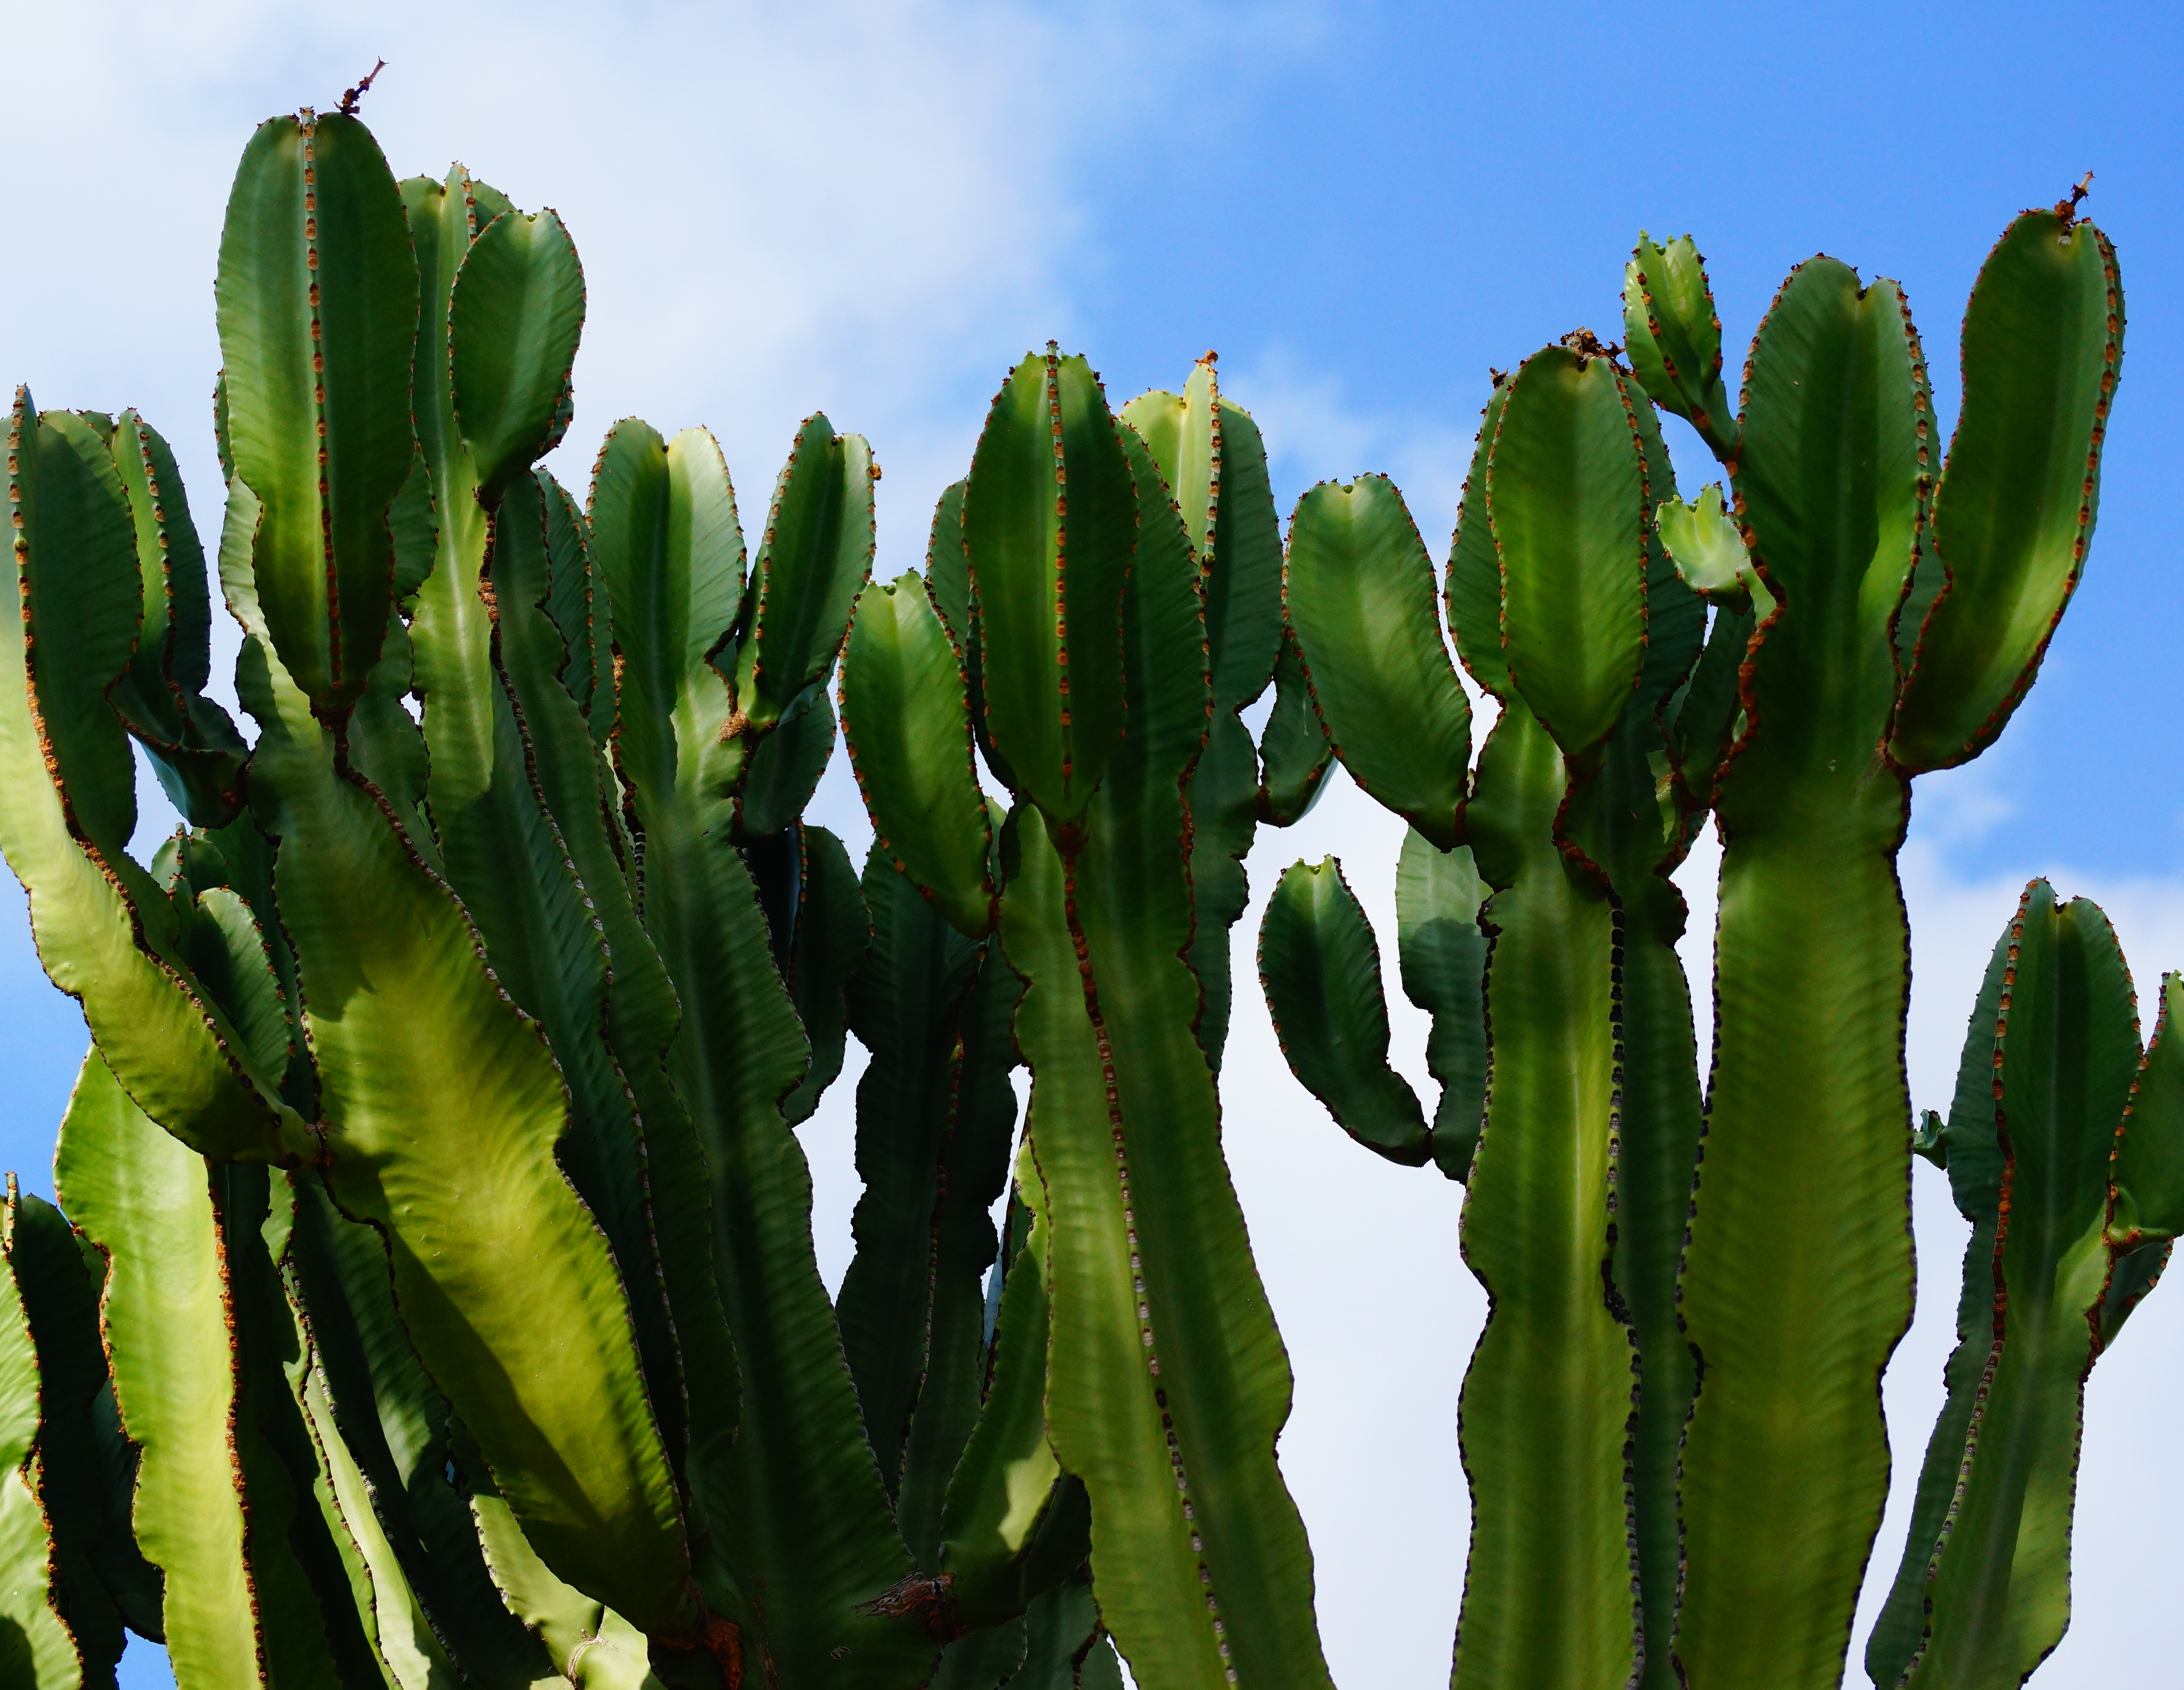
\includegraphics[width=\paperwidth,height=\paperheight]{cactus.jpg}};


\noindent
\begin{myfont}
{\huge{\xmybox[blue]{LaTeX book in \xmybox[orange]{Examples}}}} 
\end{myfont}

\vspace{0.5cm}
\vskip\baselineskip
\tikz[remember picture,overlay] \node[opacity=0.95,inner sep=0pt] at (current page.center){
\includegraphics[width=1\linewidth]{title.jpg}};
\vskip\baselineskip

\begin{myfont}
\vfill
\xmybox[green]{Thanks to me}\\
\xmybox[red]{The book is updated every week}
\end{myfont}

%-------------


\end{center}
\end{titlepage}

\clearpage
\newpage
%-------------------------------------------------------------------------------------------------------
%\vfill
%\doclicenseThis
%-------------------------------------------------------------------------------------------------------
\qbox{\bf \begin{minipage}[m]{0.4\textwidth}\centering
Support the author\\[0.3cm]
\href{https://www.buymeacoffee.com/anmnv}{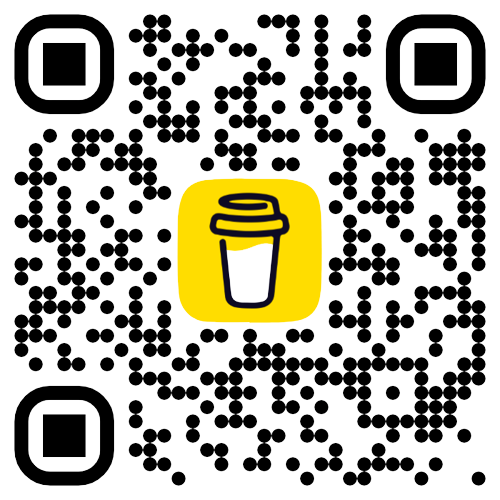
\includegraphics[width=4.5cm]{bmc_qr.png}}
\end{minipage}
\hfill
\begin{minipage}[m]{0.55\textwidth}\centering
Find it on Github\\[0.4cm]
\qrcode[height=4.3cm]{https://github.com/AnMnv/eBook}
\end{minipage} }


%------------------------------------------------------------------------------------------------------------------
\pagecolor{white}
\tableofcontents




%------------------C1-Math Tips
\chapter{Math Tips}
%-------------------1.1
\subsection{\hll{Auto-resizing equation}}
\begin{tabular}{l | c}
\begin{minipage}[m]{0.4\textwidth}
\enum{
\resizebox{.6\textwidth}{!}{$\dot{\rho}=
\dfrac{x^3}{45a^9-23b}$}}{1.1}
\end{minipage}
& \begin{minipage}[m]{0.55\textwidth}
\renewcommand\textminus{\mbox{-}}%<<<<<<<<<<<
\begin{lstlisting}[numberstyle=\zebra{black!5}{blue!15},numbers=left,basicstyle=\ttfamily\footnotesize] 
\documentclass{article}
\usepackage{amsmath}
\usepackage{graphicx}

\begin{document}
\begin{equation*}\label{eq1}
\resizebox{.4\textwidth}{!}{ % change .4 to 0.5...
$\dot{\rho}=\dfrac{x^3}{45a^9-23b}$} 
\end{equation*}
\end{document}
\end{lstlisting}
\end{minipage}
\end{tabular}
 
 

%-------------------1.2
\subsection{\hll{Form for simplest calculation}}
\begin{tabular}{l | c}
\begin{minipage}[m]{0.4\textwidth}
\enum{ \newcommand{\sss}[1]{this.getField("#1").value}
\begin{Form}
\noindent%
Fill with number \\ 
\small{\mybox[red]{if it does't work try another PDF viewer}}\\ 

\TextField[name=a]{a:} \\

\TextField[name=b]{b:} \\

\TextField[name=c]{c:} \\

\noindent%
$\sum = $ \TextField[name=AvgStat, calculate={
  event.value = ( 
    \sss{a} +
    \sss{b} +
    \sss{c}) ;
}, readonly, value=0]{} 
\end{Form}}{1.2}
\end{minipage}
& \begin{minipage}[m]{0.55\textwidth}
\renewcommand\textminus{\mbox{-}}%<<<<<<<<<<<
\begin{lstlisting}[numberstyle=\zebra{black!5}{blue!15},numbers=left,basicstyle=\ttfamily\footnotesize]{tex}
\documentclass{article}
\usepackage{hyperref}

\begin{document}
\newcommand{\sss}[1]{this.getField("#1").value}
\begin{Form}
\noindent%
Fill with number\\ 

\TextField[name=a]{a:} \\

\TextField[name=b]{b:} \\

\TextField[name=c]{c:} \\
\noindent%
$\sum = $ \TextField[name=AvgStat, calculate={
  event.value = ( 
    \sss{a} +
    \sss{b} +
    \sss{c}) ;
}, readonly, value=0]{} 
\end{Form}
\end{document}
\end{lstlisting}
\end{minipage}
\end{tabular}


%-------------------1.3
\subsection{\hll{Equation in the form of steps}}
\begin{tabular}{l | c}
\begin{minipage}[m]{0.4\textwidth}
\enum{ \resizebox{.4\textwidth}{!}{$  \frac{n_0}{n_1} = q_1 + \dfrac{\makebox[\mywd][l]{$1$}}
  {\makebox[\mywd][l]{$q_2 + \dfrac{\makebox[\mywd][l]{$1$}}
  {\makebox[\mywd][l]{$q_3 + \dfrac{\makebox[\mywd][l]{$1$}}
  {\makebox[\mywd][l]{$q_4 + 
   \raisebox{-6pt}{$\ddots$}
   \raisebox{-12pt}{+$\dfrac{\makebox[\mywd][l]{$1\kern30pt$}}
  {q_{k-1} + \dfrac{1}
  {q_k}}$}$}}$}}$}} $}}{1.3}
\end{minipage}
& \begin{minipage}[m]{0.55\textwidth}
\renewcommand\textminus{\mbox{-}}%<<<<<<<<<<<
\begin{lstlisting}[numberstyle=\zebra{black!5}{blue!15},numbers=left,basicstyle=\ttfamily\footnotesize]{tex}
\documentclass{article}
\usepackage{amsmath}
\def\mywd{35pt}

\begin{document}
\[
  \frac{n_0}{n_1} = q_1 + \dfrac{\makebox[\mywd][l]{$1$}}
  {\makebox[\mywd][l]{$q_2 + \dfrac{\makebox[\mywd][l]{$1$}}
  {\makebox[\mywd][l]{$q_3 + \dfrac{\makebox[\mywd][l]{$1$}}
  {\makebox[\mywd][l]{$q_4 + 
   \raisebox{-6pt}{$\ddots$}
   \raisebox{-12pt}{+$\dfrac{\makebox[\mywd][l]{$1\kern30pt$}}
  {q_{k-1} + \dfrac{1}
  {q_k}}$}$}}$}}$}}
\]
\end{document}
\end{lstlisting}
\end{minipage}
\end{tabular}

%-------------------1.4
\subsection{\hll{One number for multiline equation}}
\begin{tabular}{l | c}
\begin{minipage}[m]{0.4\textwidth}
\enum{ \begin{equation}
\begin{aligned}
x_{ij} &= d_{ijk}E_k, \\ 
x_{ij} &= \varsigma_{ijk}H_k,\\ 
x_{ij} &= s_{ijkl}X_{kl},\\ 
x_{ij} &= \xi_{ij}\delta p,\\ 
x_{ij} &= \alpha_{ij}\delta T
\end{aligned}
\end{equation}}{1.4}
\end{minipage}
& \begin{minipage}[m]{0.55\textwidth}
\renewcommand\textminus{\mbox{-}}%<<<<<<<<<<<
\begin{lstlisting}[numberstyle=\zebra{black!5}{blue!15},numbers=left,basicstyle=\ttfamily\footnotesize]{tex}
\documentclass{article}
\usepackage{amsmath}

\begin{document}
\begin{equation}
\begin{aligned}
x_{ij} &= d_{ijk}E_k, \\ 
x_{ij} &= \varsigma_{ijk}H_k,\\ 
x_{ij} &= s_{ijkl}X_{kl},\\ 
x_{ij} &= \xi_{ij}\delta p,\\ 
x_{ij} &= \alpha_{ij}\delta T
\end{aligned}
\end{equation}
\end{document}
\end{lstlisting}
\end{minipage}
\end{tabular}

%-------------------1.5
\subsection{\hll{Matrix in \textbf{standalone} documentclass}}
\begin{tabular}{l | c}
\begin{minipage}[m]{0.4\textwidth}
\enum{ \begin{equation*}
\begin{matrix} 
a_{11} & a_{12} & a_{13}  \\
a_{21} & a_{22} & a_{23}  \\
a_{31} & a_{32} & a_{33}  \\
\end{matrix} 
\end{equation*} }{1.5}
\end{minipage}
& \begin{minipage}[m]{0.55\textwidth}
\renewcommand\textminus{\mbox{-}}%<<<<<<<<<<<
\begin{lstlisting}[numberstyle=\zebra{black!5}{blue!15},numbers=left,basicstyle=\ttfamily\footnotesize]{tex}
\documentclass[preview,border={-5cm 0cm -5cm -0.1cm}]{standalone}
\usepackage{amsmath}

\begin{document}
\begin{equation*}
\begin{matrix} 
a_{11} & a_{12} & a_{13}  \\
a_{21} & a_{22} & a_{23}  \\
a_{31} & a_{32} & a_{33}  \\
\end{matrix} 
\end{equation*}
\end{document}
\end{lstlisting}
\end{minipage}
\end{tabular}


%-------------------1.6
\subsection{\hll{Multiple lines, one centered label}}
\begin{tabular}{l | c}
\begin{minipage}[m]{0.4\textwidth}
\enum{ \begin{equation} \label{eq1}
\begin{split}
A & = \frac{\pi r^2}{2} \\
 & = \frac{1}{2} \pi r^2
\end{split}
\end{equation} }{1.6}
\end{minipage}
& \begin{minipage}[m]{0.55\textwidth}
\renewcommand\textminus{\mbox{-}}%<<<<<<<<<<<
\begin{lstlisting}[numberstyle=\zebra{black!5}{blue!15},numbers=left,basicstyle=\ttfamily\footnotesize] 
\begin{equation} \label{eq1}
\begin{split}
A & = \frac{\pi r^2}{2} \\
 & = \frac{1}{2} \pi r^2
\end{split}
\end{equation}
\end{lstlisting}
\end{minipage}
\end{tabular}

%-------------------1.7
\subsection{\hll{Array as a fraction}}
\begin{tabular}{l | c}
\begin{minipage}[m]{0.4\textwidth}
\enum{ 
$I-IV-V^{\substack{6-4\\4-3\\6-4\\4-3}}-I-cadence$ \\

$I-IV-V^{\genfrac{}{}{0pt}{}{6-4}{4-3}}-I-cadence$ \\

$I-IV-V^{\begin{array}{c}6-4\\4-3\\ \end{array}}-I-cadence$}{1.7}
\end{minipage}
& \begin{minipage}[m]{0.55\textwidth}
\renewcommand\textminus{\mbox{-}}%<<<<<<<<<<<
\begin{lstlisting}[numberstyle=\zebra{black!5}{blue!15},numbers=left,basicstyle=\ttfamily\footnotesize] 
\documentclass{article}
\usepackage{amsmath}

\begin{document}
$I-IV-V^{\substack{6-4\\4-3\\6-4\\4-3}}-I-cadence$ \\

$I-IV-V^{\genfrac{}{}{0pt}{}{6-4}{4-3}}-I-cadence$ \\

$I-IV-V^{\begin{array}{c}6-4\\4-3\\ \end{array}}-I-cadence$
\end{document}
\end{lstlisting}
\end{minipage}
\end{tabular}

%-------------------1.8
\subsection{\hll{Aligning equations inbetween text}}
\begin{tabular}{l | c}
\begin{minipage}[m]{0.4\textwidth}
\begin{tcblisting}{colback=white,colframe=white,comment style={frame hidden,scale=2.5}, comment only, pdf comment, freeze pdf, compilable listing, run pdflatex,}
\documentclass[varwidth, border={10pt 10pt 10pt 10pt}]{standalone}
\usepackage{amsmath}
\begin{document}
qqq
\end{document}
\end{tcblisting}
\end{minipage}
& \begin{minipage}[m]{0.55\textwidth}
\renewcommand\textminus{\mbox{-}}%<<<<<<<<<<<
\begin{lstlisting}[numberstyle=\zebra{black!5}{blue!15},numbers=left,basicstyle=\ttfamily\footnotesize] 
\documentclass{article}
\usepackage{amsmath}

\begin{document}
\begin{alignat*}{2}
\intertext{Photochemical:}
K_{UV} &: M[1]& &\ch{-> M^{*}}[1]
\intertext{Catalyzed:}
K_I &: I& &\ch{->} 2R \\
K_S &: R + M [1]& &\ch{-> RM^{*}}[1]
\end{alignat*}
\end{document} 
\end{lstlisting}
\end{minipage}
\end{tabular}

%-------------------1.9
\subsection{\hll{Equation: boxed split inside align}}
\begin{tabular}{l | c}
\begin{minipage}[m]{0.4\textwidth}
\begin{tikzpicture}
\node (0,0) {\begin{minipage}[m]{0.90\textwidth}
\begin{tcblisting}{colback=white,colframe=white,comment style={frame hidden,scale=2.5}, comment only, pdf comment, freeze pdf, compilable listing, run pdflatex,}
\documentclass[varwidth, border={-120pt 10pt 10pt 10pt}]{standalone}
\usepackage{mathtools}
\usepackage{xcolor}

\begin{document}
\begin{align}
    \begin{split}
        A ={}& B + C + D
    \end{split}\nonumber\\
  \mathrlap{\boxed{\phantom{\begin{gathered}A = {}+ C\_is\_long\_too\\A\\A\end{gathered}}}}
  \hspace{\dimexpr\fboxsep+\fboxrule-0.4pt}
  \begin{split}
        A ={}& \phantom{{}+{}} B\_is\_long\\
             &            +    C\_is\_long\_too\\
             &            +    D\_is\_long\_too
    \end{split}
\end{align}
\end{document}
\end{tcblisting}
\end{minipage}};
\node [opacity=0.05] (0,0) {\scalebox{8.0}{\textcolor{red}{1.9}}};
\end{tikzpicture}
\end{minipage} 
&
\begin{minipage}[m]{0.55\textwidth}
\begin{lstlisting}[numberstyle=\zebra{black!5}{blue!15},numbers=left,basicstyle=\ttfamily\footnotesize] 
\begin{document}
\begin{align}
\begin{split}
A ={}& B + C + D
\end{split}\nonumber\\
\mathrlap{\boxed{\phantom{\begin{gathered}A = {}+ C\_is\_long\_too\\A\\A\end{gathered}}}}
\hspace{\dimexpr\fboxsep+\fboxrule-0.4pt}
\begin{split}
A ={}& \phantom{{}+{}} B\_is\_long\\
&  +    C\_is\_long\_too\\
&  +    D\_is\_long\_too
\end{split}
\end{align}
\end{document}
\end{lstlisting}
\end{minipage}
\end{tabular}

%-------------------1.10
\subsection{\hll{Multiline text above arrow or relation symbol}}
\begin{tabular}{l | c}
\begin{minipage}[m]{0.4\textwidth}
\begin{tikzpicture}
\node (0,0) {\begin{minipage}[m]{0.90\textwidth}
\begin{tcblisting}{colback=white,colframe=white,comment style={frame hidden,scale=2.5}, comment only, pdf comment, freeze pdf, compilable listing, run pdflatex,}
\documentclass[varwidth, border={5pt 5pt 5pt 5pt}]{standalone}
\usepackage{mathtools}
\newcommand{\twoline}[2]{\overset{\textup{\scriptsize #1}}{\textup{#2}}}

\begin{document}
$$\dfrac{x+1}{x} \xrightarrow{\twoline{Euclidean}{division}} 1+\dfrac{1}{x}$$
\end{document}
\end{tcblisting}
\end{minipage}};
\node [opacity=0.05] (0,0) {\scalebox{8.0}{\textcolor{red}{1.10}}};
\end{tikzpicture}
\end{minipage} 
&
\begin{minipage}[m]{0.55\textwidth}
\begin{lstlisting}[numberstyle=\zebra{black!5}{blue!15},numbers=left,basicstyle=\ttfamily\footnotesize] 
\documentclass[a4paper, 12pt]{article}
\usepackage{mathtools}
\newcommand{\twoline}[2]{\overset{\textup{\scriptsize #1}}{\textup{#2}}}

\begin{document}
\begin{equation*}
\dfrac{x+1}{x} \xrightarrow{\twoline{Euclidean}{division}} 1+\dfrac{1}{x}
\end{equation*}
\end{document}
\end{lstlisting}
\end{minipage}
\end{tabular}

%-------------------1.11
%-------------------1.12
%-------------------1.13
%-------------------1.14


 


 
%------------------C2-Sybols
\chapter{Text, Symbols}
\section{New section symbol}
%-------------------2.1
\begin{table}[h!]
\begin{tabular}{c | c}
\begin{minipage}[m]{0.4\textwidth}
\enum{\sectionlinetwo{orange}{88}}{2.1}
\end{minipage}
&
\begin{minipage}[m]{0.55\textwidth}
\renewcommand\textminus{\mbox{-}}%<<<<<<<<<<<
\begin{lstlisting}[numberstyle=\zebra{red!15}{black!10},numbers=left,basicstyle=\footnotesize]{tex}
\usepackage[object=vectorian]{pgfornament}  
\usepackage{lipsum,tikz}
\newcommand{\sectionlinetwo}[2]{%
\nointerlineskip \vspace{.5\baselineskip}\hspace{\fill}
{\color{#1}\resizebox{0.5\linewidth}{2ex}
{{{\begin{tikzpicture}
\node  (C) at (0,0) {};\node (D) at (9,0) {};
\path (C) to [ornament=#2] (D);
\end{tikzpicture}}}}}%
\hspace{\fill}\par\nointerlineskip 
\vspace{.5\baselineskip}}
%usage---> \sectionlinetwo{orange}{88}
\end{lstlisting}
\end{minipage}
\end{tabular}
\end{table}


%-------------------2.2
\section{Wireframe rendering}
\begin{table}[h!]
\begin{tabular}{c | c}
\begin{minipage}[m]{0.4\textwidth}
\enum{ \roboto\huge\contourlength{.15em}
\contour{gray}{boxed} \contour{red}{boxed} \contour{yellow}{boxed}}{2.2}
\end{minipage}
&
\begin{minipage}[m]{0.55\textwidth}
\renewcommand\textminus{\mbox{-}}%<<<<<<<<<<<
\begin{lstlisting}[numberstyle=\zebra{red!15}{black!10},numbers=left,basicstyle=\footnotesize] 
\documentclass{article}
\usepackage{xcolor}
\usepackage{roboto}
\usepackage[outline]{contour}
\begin{document}
\roboto\huge\contourlength{.15em}
\contour{gray}{boxed}
\end{document}
\end{lstlisting}
\end{minipage}
\end{tabular}
\end{table}

%-------------------2.3
\section{Justifyed text}
\begin{table}[h!]
\begin{tabular}{c | c}
\begin{minipage}[m]{0.4\textwidth}
\enum{\texttt{\justify\blindenumerate[10]}}{2.3}
\end{minipage}
&
\begin{minipage}[m]{0.55\textwidth}
\renewcommand\textminus{\mbox{-}}%<<<<<<<<<<<
\begin{lstlisting}[numberstyle=\zebra{red!15}{black!10},numbers=left,basicstyle=\footnotesize] 
\documentclass{article}
\usepackage{blindtext}
\newcommand*\justify{%
  \fontdimen2\font=0.4em% interword space
  \fontdimen3\font=0.2em% interword stretch
  \fontdimen4\font=0.1em% interword shrink
  \fontdimen7\font=0.1em% extra space
  \hyphenchar\font=`\-% allowing hyphenation
}

\begin{document}
\texttt{\justify\blindenumerate[10]}
\end{document}
\end{lstlisting}
\end{minipage}
\end{tabular}
\end{table}


%-------------------2.4
\section{Text under an underline}
\begin{table}[h!]
\begin{tabular}{c | c}
\begin{minipage}[m]{0.4\textwidth}
\enum{
\includegraphics[width=\linewidth]{2.4.png} }{2.4}
\end{minipage}
&
\begin{minipage}[m]{0.55\textwidth}
\renewcommand\textminus{\mbox{-}}%<<<<<<<<<<<
\begin{lstlisting}[numberstyle=\zebra{red!15}{black!10},numbers=left,basicstyle=\footnotesize] 
\documentclass[12pt]{article}
\usepackage{amsmath,soul}
\usepackage{soulpos}
\ulposdef{\ulnumaux}{%
$\underset{\saveulnum}{\rule[-.7ex]{\ulwidth}{.4pt}}$}
\newcommand{\ulnum}[2]{%
\def\saveulnum{#1}%
\ulnumaux{#2}}

\begin{document} 
\ulnum{\text{(some text)}}{This is short text}
\end{document}
\end{lstlisting}
\end{minipage}
\end{tabular}
\end{table}
%-------------------2.5
\section{Bullets Style}
\begin{table}[h!]
\begin{tabular}{c | c}
\begin{minipage}[m]{0.4\textwidth}
\enum{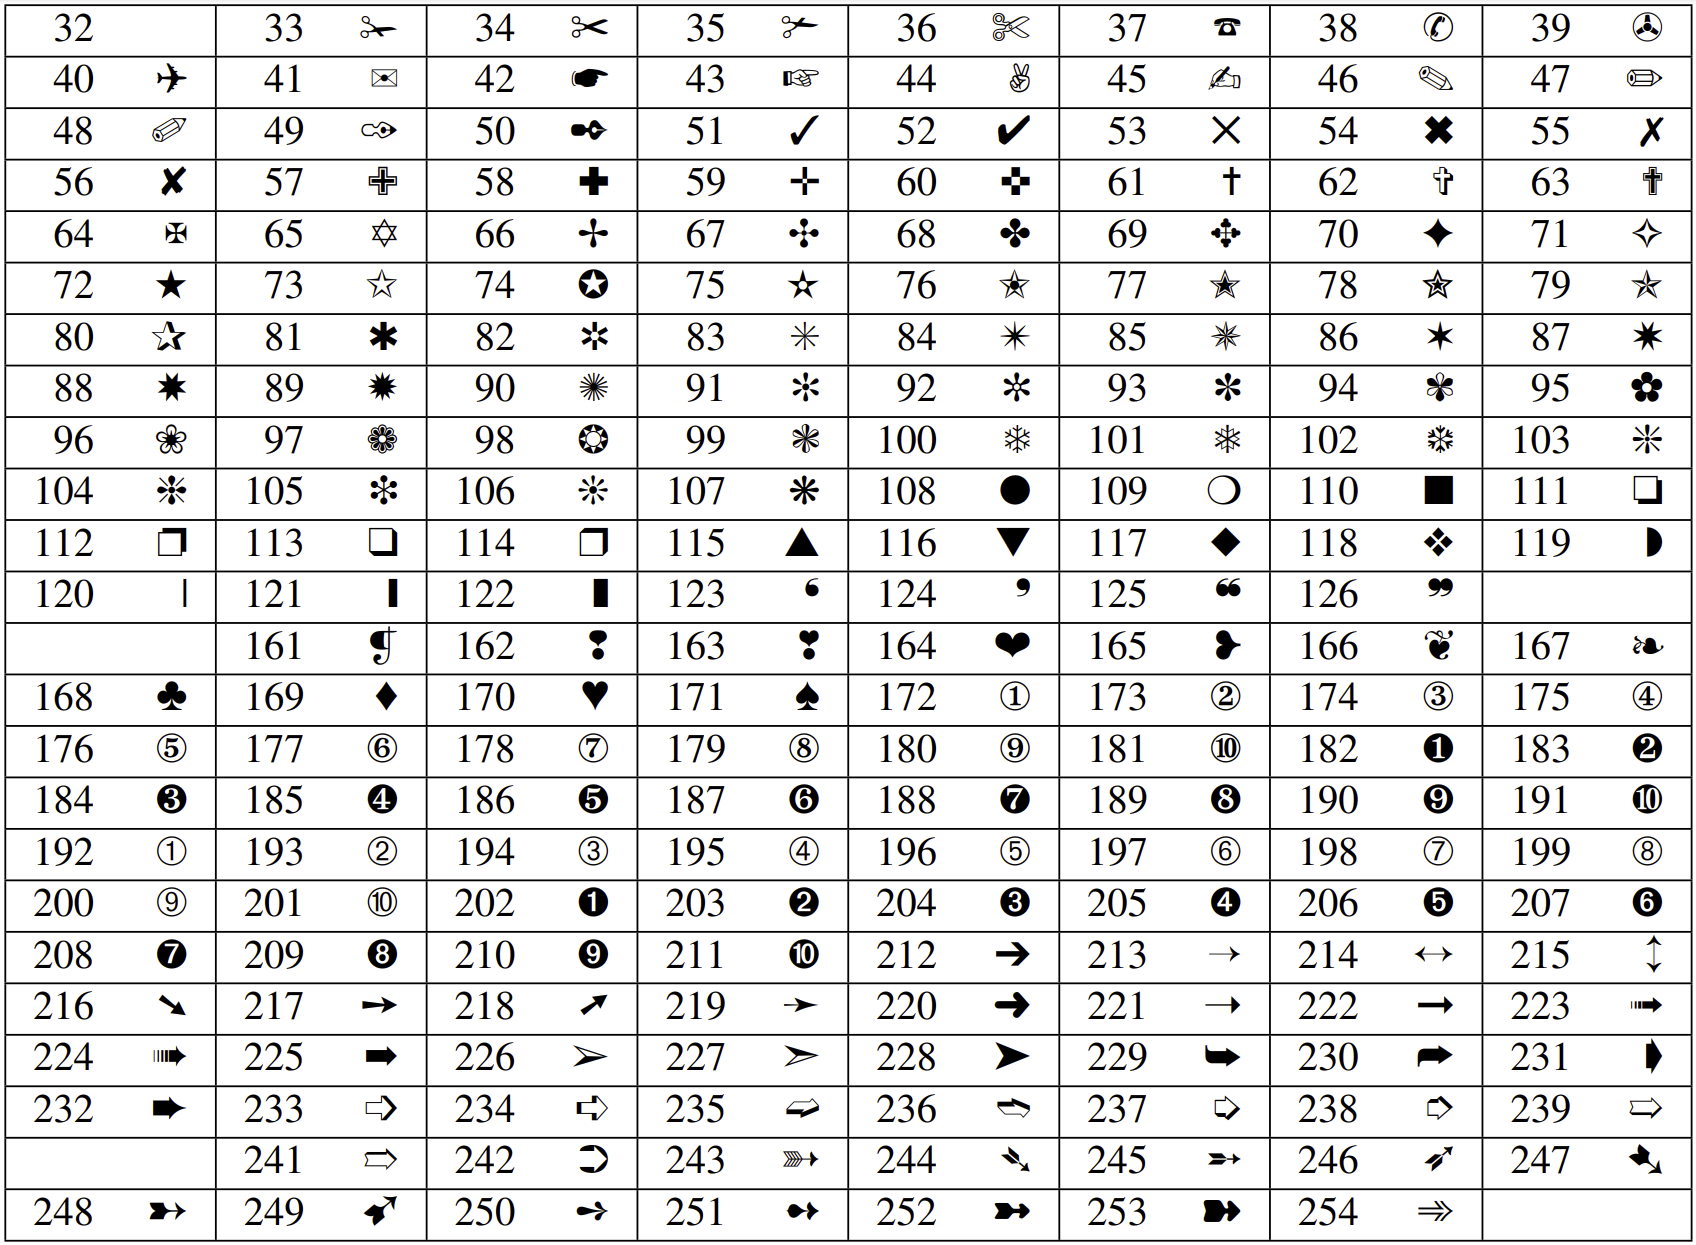
\includegraphics[width=\linewidth]{2.5.png} }{2.4}
\end{minipage}
&
\begin{minipage}[m]{0.55\textwidth}
\renewcommand\textminus{\mbox{-}}%<<<<<<<<<<<
\begin{lstlisting}[numberstyle=\zebra{red!15}{black!10},numbers=left,basicstyle=\footnotesize] 
\documentclass{article}
\usepackage{pifont}

\begin{document}
\begin{itemize}
    \item[\ding{51}] Code 51
    \item[\ding{56}] Code 56
    \item[\ding{43}] Code 43
    \item[\ding{118}] Code 118
    \item[\ding{170}] Code 170
\end{itemize}
\ding{46} \ding{70} \ding{57}  \ding{98} \ding{96}
\end{document}
\end{lstlisting}
\end{minipage}
\end{tabular}
\end{table}
%-------------------2.6
%-------------------2.7








%------------------C3-Listing
\chapter{Code, listings, minted \dots}
%-------------------3.1
\subsection{\hll{Code listing using \xmyboxg{minted} in \xmyboxg{beamer}}}
\begin{table}[h!]
\begin{tabular}{c | c}
\begin{minipage}[m]{0.4\textwidth}
\enum{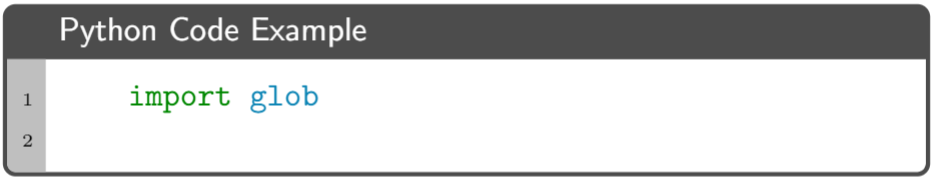
\includegraphics[width=1\linewidth]{3.1.png}}{3.1}
\end{minipage}
&
\begin{minipage}[m]{0.55\textwidth}
\renewcommand\textminus{\mbox{-}}%<<<<<<<<<<<
\begin{lstlisting}[numberstyle=\zebra{pink!15}{green!15},numbers=left,basicstyle=\ttfamily\footnotesize]{tex}
\documentclass{beamer}
\usepackage{tcolorbox}
\tcbuselibrary{minted,skins,breakable}
\newtcblisting{pythoncode}[2][]{
  listing engine=minted, breakable,  colback=bg,
  colframe=black!70,  listing only,
  minted style=colorful,  minted language=python,
  minted options={numbersep=3mm,texcl=true,#1},
  left=5mm,enhanced,
  overlay={\begin{tcbclipinterior}\fill[black!25] (frame.south west)
rectangle ([xshift=5mm]frame.north west);\end{tcbclipinterior}},
#2,}
\begin{document}
\begin{frame}[fragile]
    \frametitle{Premature Optimization}
    \begin{pythoncode}[linenos=true,]{title=Python Code Example}
    import glob
    \end{pythoncode}
\end{frame}
\end{document}
\end{lstlisting}
\end{minipage}
\end{tabular}
\end{table}

%-------------------3.2
\subsection{\hll{"Zebra" style listing}}
\begin{table}[h!]
\begin{tabular}{c | c}
\begin{minipage}[m]{0.4\textwidth}
 \begin{lstlisting}[numberstyle=\zebra{green!25}{yellow!25},numbers=left,basicstyle=\ttfamily\footnotesize]
/**
* Prints Hello World.
**/
#include <stdio.h>

int main(void) {
   printf("Hello World!");
   return 0;
}
\end{lstlisting} 
\end{minipage}
&
\begin{minipage}[m]{0.55\textwidth}
\renewcommand\textminus{\mbox{-}}%<<<<<<<<<<<
\begin{tiny}
\begin{verbatim}
\documentclass{article}
\usepackage[T1]{fontenc}
\usepackage{beramono}
\usepackage{listings}
\usepackage{xcolor}
\newcommand\realnumberstyle[1]{}
\makeatletter
\newcommand{\zebra}[3]{%
    {\realnumberstyle{#3}}%
    \begingroup
    \lst@basicstyle
    \ifodd\value{lstnumber}%
        \color{#1}%
    \else
        \color{#2}%
    \fi
        \rlap{\hspace*{\lst@numbersep}%
        \color@block{\linewidth}{\ht\strutbox}{\dp\strutbox}%
        }%
    \endgroup}
\makeatother
\begin{document}
\begin{lstlisting}[language=C,basicstyle=\ttfamily,
numberstyle=\zebra{green!35}{yellow!35},numbers=left]
/**
* Prints Hello World.
**/
#include <stdio.h>
int main(void) {
   printf("Hello World!");
   return 0;
}
\end{lstlisting}
\end{document}
\end{verbatim}
\end{tiny}
\end{minipage}
\end{tabular}
\end{table}
\clearpage

%-------------------3.3

\subsection{\hll{Listing with russian language}}
\begin{table}[h!]
\begin{tabular}{c | c}
\begin{minipage}[m]{0.4\textwidth}
\enum{ 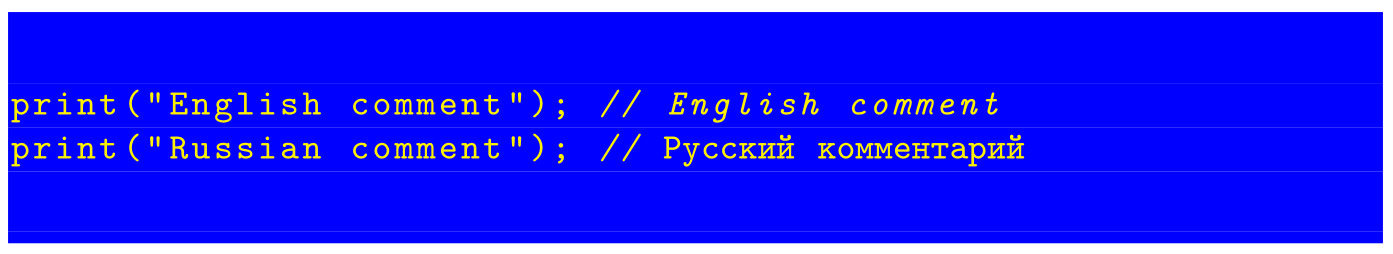
\includegraphics[width=1\linewidth]{3.3.png} }{3.3}
\end{minipage}
&
\begin{minipage}[m]{0.55\textwidth}
\renewcommand\textminus{\mbox{-}}%<<<<<<<<<<<
\begin{lstlisting}[numberstyle=\zebra{pink!15}{green!15},numbers=left,basicstyle=\ttfamily\footnotesize] 
\documentclass{article}
\usepackage[T2A]{fontenc}
\usepackage[utf8]{inputenc}
\usepackage[russian]{babel}
\usepackage{listings} 
\usepackage{xcolor}

\begin{document}
\lstset{ keepspaces=true, 
backgroundcolor=\color{blue},  
showstringspaces=false, 
language=C, 
extendedchars=\true, 
framexrightmargin=0pt,
framexleftmargin=0pt,
framextopmargin=15pt,
framexbottommargin=15pt, 
frame=tb, framerule=0pt,
basicstyle=\color{yellow}\ttfamily\small}

begin{lstlisting}% <<<<<<<<< add "/"
print("English comment"); // English comment
print("Russian comment"); // %here can be russian words
end{lstlisting}%   <<<<<<<<< add "/"
\end{document}
\end{lstlisting}
\end{minipage}
\end{tabular}
\end{table}
 
%-------------------3.4
\subsection{\hll{Listing with \xmyboxg{minted}}}
\begin{table}[h!]
\begin{tabular}{c | c}
\begin{minipage}[m]{0.4\textwidth}
\enum{ \href{https://tex.stackexchange.com/questions/174455/typeset-source-code-with-tcolorbox}{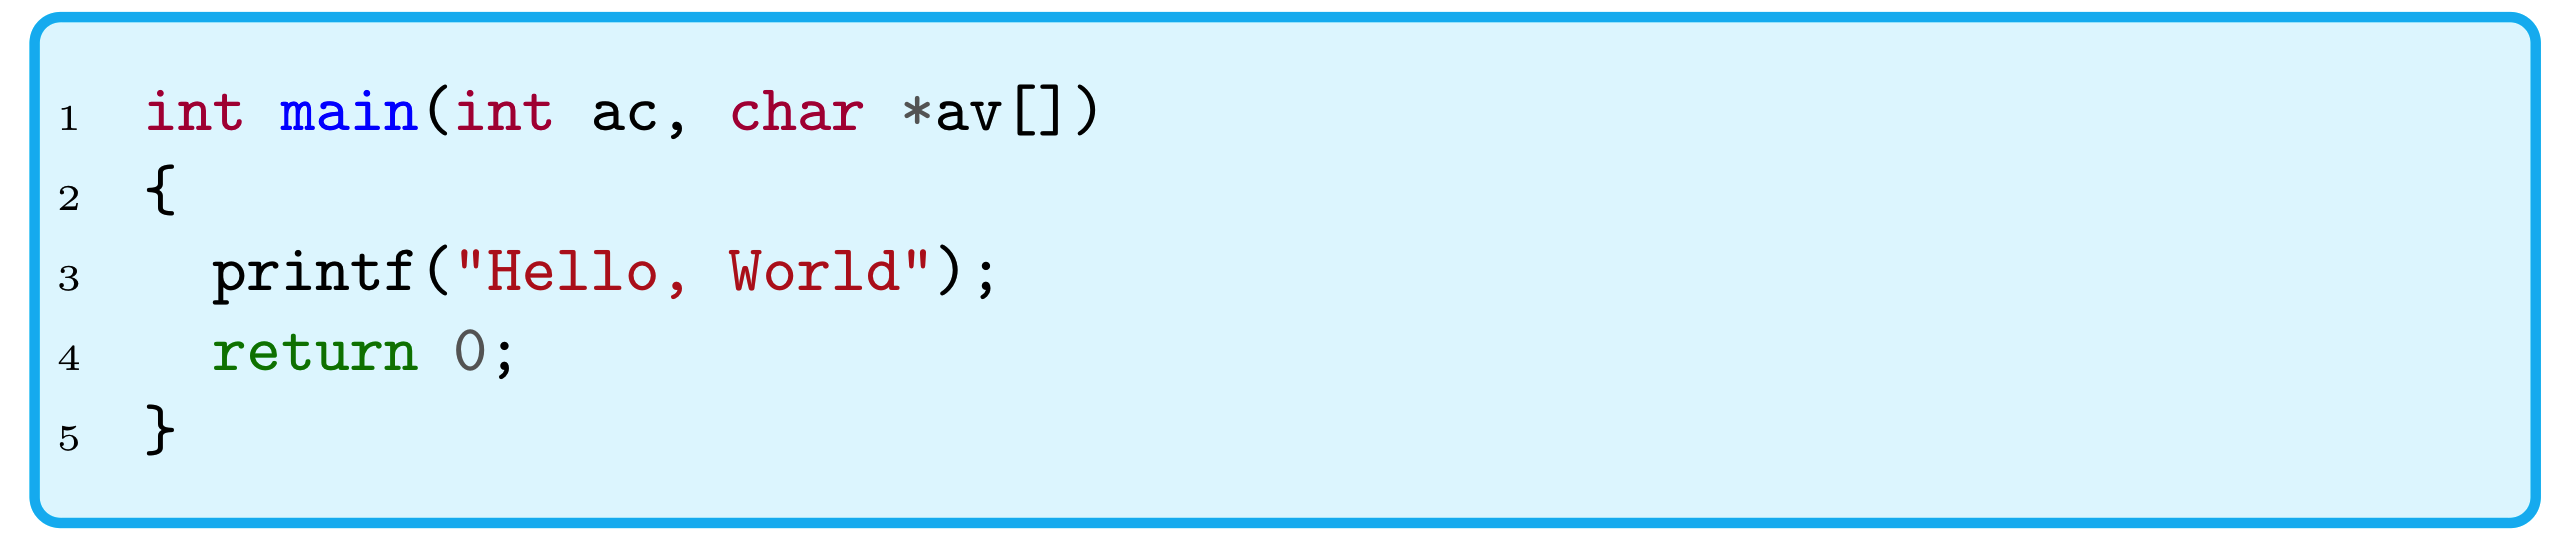
\includegraphics[width=1\linewidth]{3.4.png}} }{3.4}
\end{minipage}
&
\begin{minipage}[m]{0.55\textwidth}
\renewcommand\textminus{\mbox{-}}%<<<<<<<<<<<
\begin{lstlisting}[numberstyle=\zebra{pink!15}{green!15},numbers=left,basicstyle=\ttfamily\footnotesize] 
\documentclass{article}
\usepackage[many]{tcolorbox}
\tcbuselibrary{minted}
\newtcblisting{mylisting}{
  colframe=cyan,
  colback=cyan!10,
  listing only,
  listing engine=minted,
  minted language=cpp,
  minted options={fontsize=\small,linenos,numbersep=3mm},
}

\begin{document}
\begin{mylisting}
some code 
\end{mylisting}
\end{document}
\end{lstlisting}
\end{minipage}
\end{tabular}
\end{table}
%\enum{\href{https://tex.stackexchange.com/questions/670255/remove-thin-black-frame-around-standalone-image/670257#670257}{%}{3.5}
%-------------------3.5
\subsection{\hll{Run LaTeX code inside and show result}}
\begin{table}[h!]
\begin{tabular}{c | c}
\begin{minipage}[m]{0.4\textwidth}
\begin{tikzpicture}
\node (0,0) {\begin{minipage}[m]{0.90\textwidth}
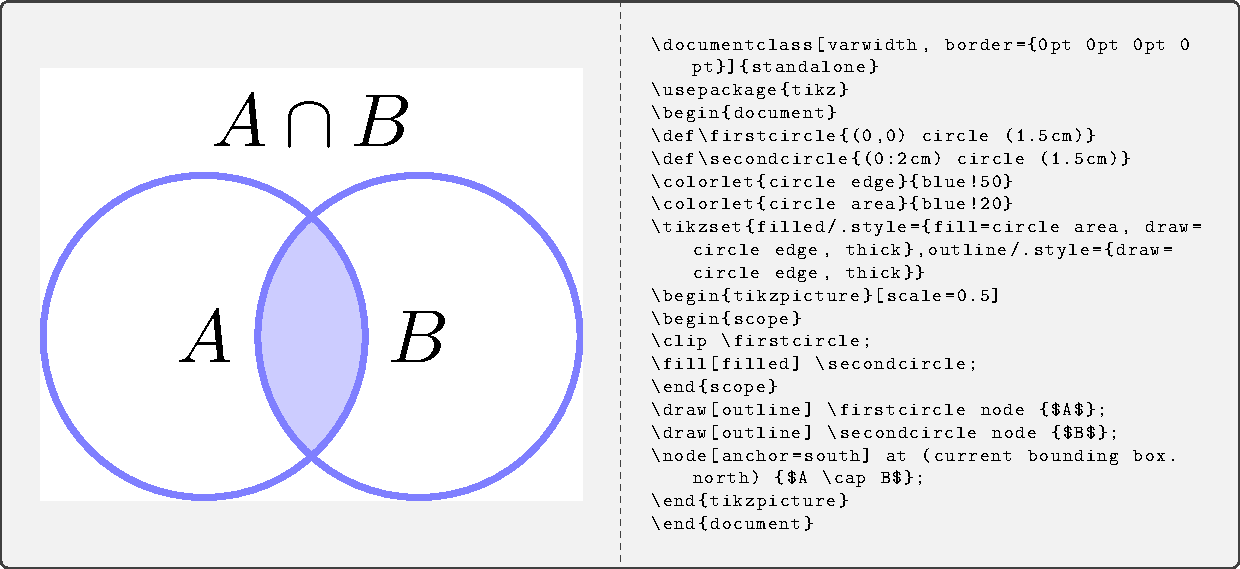
\includegraphics[width=1\linewidth]{C:/Users/user/Desktop/eBook/images/3.5.pdf}
\end{minipage} };
\node [opacity=0.05] (0,0) {\scalebox{8.0}{\textcolor{red}{\emph{3.5}}}};
\end{tikzpicture}
\end{minipage}
&
\begin{minipage}[m]{0.55\textwidth}
\renewcommand\textminus{\mbox{-}}%<<<<<<<<<<<
\begin{lstlisting}[numberstyle=\zebra{pink!15}{green!15},numbers=left,basicstyle=\ttfamily\footnotesize] 
\documentclass{standalone}
\usepackage[most]{tcolorbox}
\tcbset{sidebyside,width = 21cm,listing options={basicstyle=\small\ttfamily,breaklines=true}}
 
\begin{document}
\begin{tcblisting}{comment and listing, pdf comment, freeze pdf, compilable listing, run pdflatex, comment style={frame hidden,scale=2}}
\documentclass[varwidth, border={0pt 0pt 0pt 0pt}]{standalone}
\usepackage{tikz}
\begin{document}
\def\firstcircle{(0,0) circle (1.5cm)}
\def\secondcircle{(0:2cm) circle (1.5cm)}
\colorlet{circle edge}{blue!50}
\colorlet{circle area}{blue!20}
\tikzset{filled/.style={fill=circle area, draw=circle edge, thick},outline/.style={draw=circle edge, thick}}
\begin{tikzpicture}[scale=0.5]
\begin{scope}
\clip \firstcircle;
\fill[filled] \secondcircle;
\end{scope}
\draw[outline] \firstcircle node {$A$};
\draw[outline] \secondcircle node {$B$};
\node[anchor=south] at (current bounding box.north) {$A \cap B$};
\end{tikzpicture}
\end{document}
\end{tcblisting}
\end{document}
\end{lstlisting}
\end{minipage}
\end{tabular}
\end{table}

%-------------------3.6
\subsection{\hll{Breaking code lines in a tcolorbox}}
\begin{tabular}{l | c}
\begin{minipage}[m]{0.4\textwidth}
\begin{tikzpicture}
\node (0,0) {\begin{minipage}[m]{0.90\textwidth}
\begin{tcblisting}{colback=white,colframe=white,comment style={frame hidden,scale=2.5}, comment only, pdf comment, freeze pdf, compilable listing, run pdflatex,}
\documentclass[varwidth, border={10pt 10pt 10pt 10pt}]{standalone}
\usepackage{hyperref}
\usepackage[table]{xcolor}
\usepackage{listings}
\usepackage[most]{tcolorbox}
\usepackage{inconsolata}
\usepackage{graphicx}
\tcbuselibrary{breakable}

\newtcblisting[auto counter,number within=chapter]{sourcecode}[2][]{sharp corners, breakable,
    fonttitle=\bfseries, colframe=gray, listing only, 
    listing options={basicstyle=\ttfamily,language=php, showstringspaces=false, 
    breaklines=true, postbreak={\raisebox{0ex}[0ex][0ex]{\ensuremath{\color{red}\hookrightarrow\space}}}, tabsize=4
  }, 
    title=Code Snippet \thetcbcounter: #2, #1}


\begin{document}

\begin{sourcecode}{}
    <?php

    function abc($file_name){

        header('Content-Type: application/vnd.openxmlformats-officedocument.spreadsheetml.sheet');
        header('Content-Disposition: attachment;filename="'.$file_name.'"');
        header('Cache-Control: max-age=0');
        $writer->save('php://output');
    }

\end{sourcecode}

\end{document}
\end{tcblisting}
\end{minipage}};
\node [opacity=0.05] (0,0) {\scalebox{8.0}{\textcolor{red}{3.6}}};
\end{tikzpicture}
\end{minipage} 
&
\begin{minipage}[m]{0.55\textwidth}
\begin{lstlisting}[numberstyle=\zebra{black!5}{blue!15},numbers=left,basicstyle=\ttfamily\footnotesize] 
\documentclass{book}
\usepackage{hyperref}
\usepackage[table]{xcolor}
\usepackage{listings}
\usepackage[most]{tcolorbox}
\usepackage{inconsolata}
\usepackage{graphicx}
\tcbuselibrary{breakable}

\newtcblisting[auto counter,number within=chapter]{sourcecode}[2][]{sharp corners, breakable,
    fonttitle=\bfseries, colframe=gray, listing only, 
    listing options={basicstyle=\ttfamily,language=php, showstringspaces=false, 
    breaklines=true, postbreak={\raisebox{0ex}[0ex][0ex]{\ensuremath{\color{red}\hookrightarrow\space}}}, tabsize=4
  }, title=Code Snippet \thetcbcounter: #2, #1}

\begin{document}
\begin{sourcecode}{}
<?php

function abc($file_name){

header('Content-Type: application/vnd.openxmlformats-officedocument.spreadsheetml.sheet');
header('Content-Disposition: attachment;filename="'.$file_name.'"');
header('Cache-Control: max-age=0');
$writer->save('php://output');
}
\end{sourcecode}
\end{document}
\end{lstlisting}
\end{minipage}
\end{tabular}

%-------------------3.7
%https://tex.stackexchange.com/questions/452150/advanced-customization-of-minted-code
\subsection{\hll{Modern code listing using \xmyboxg{minted}}}
\begin{table}[h!]
\begin{tabular}{c | c}
\begin{minipage}[m]{0.4\textwidth}

paraiso-dark
\begin{javalst}
public class ClassName {
        public static void main(String[] args) {
            System.out.println(args);
        }
}
\end{javalst}
emacs
\begin{javalstt}
public class ClassName {
        public static void main(String[] args) {
            System.out.println(args);
        }
}
\end{javalstt}
vim
\begin{javalsttt}
public class ClassName {
        public static void main(String[] args) {
            System.out.println(args);
        }
}
\end{javalsttt} 
perldoc
\begin{javalstttt}
public class ClassName {
        public static void main(String[] args) {
            System.out.println(args);
        }
}
\end{javalstttt}
monokai
\begin{python}
public class ClassName {
        public static void main(String[] args) {
            System.out.println(args);
        }
}
\end{python}
\end{minipage}
&
\begin{minipage}[m]{0.55\textwidth}
\renewcommand\textminus{\mbox{-}}%<<<<<<<<<<<
\begin{lstlisting}[numberstyle=\zebra{pink!15}{green!15},numbers=left,basicstyle=\ttfamily\footnotesize]{tex}
\documentclass{article}
\usepackage[T1]{fontenc}
\usepackage{listings}
\usepackage{minted}
\usepackage{xcolor}
\usepackage{tcolorbox}
\tcbuselibrary{listings, minted, skins}
\tcbset{listing engine=minted}
\newtcblisting{javalst}{listing only, minted language=java, minted style=paraiso-dark,
    colback=bg, enhanced, frame hidden, minted options={fontfamily=fdm, 
    fontsize=\footnotesize, tabsize=2, breaklines, autogobble}}
\definecolor{inline}{RGB}{187,57,82}
\definecolor{bg}{RGB}{22,43,58}
\setminted[java]{bgcolor=bg, fontfamily=fdm, fontsize=\footnotesize}

\begin{document}
\begin{javalst}
    public class ClassName {
            public static void main(String[] args) {
                System.out.println(args);
            }
    }
\end{javalst}
\end{document}
\end{lstlisting}

For lines numbering (last example):

\begin{lstlisting}[numberstyle=\zebra{pink!15}{red!15},numbers=left,basicstyle=\ttfamily\scriptsize]{tex}
\documentclass{article}
\usepackage[T1]{fontenc}
\usepackage{listings}
\usepackage{minted}
\usepackage{xcolor}
\usepackage{tcolorbox}
\tcbuselibrary{listings, minted, skins}
\tcbset{listing engine=minted}
\renewcommand{\theFancyVerbLine}{\textcolor[rgb]{1,1,1}{\texttt\footnotesize\arabic{FancyVerbLine}}}
\newtcblisting{javalst}{listing only, minted language=java, minted style=paraiso-dark, colback=bg, enhanced,frame hidden,
minted options={fontsize=\footnotesize, tabsize=2, breaklines, autogobble, linenos, numbersep=5pt,fontsize=\small,},
overlay={\begin{tcbclipinterior}\fill[bg](frame.south west)rectangle([xshift=5mm]frame.north west);\end{tcbclipinterior}}}
\definecolor{inline}{RGB}{187,57,82}
\definecolor{bg}{RGB}{22,43,58}
\setminted[java]{bgcolor=bg, fontfamily=fdm, fontsize=\footnotesize}

\begin{document}
\begin{javalst}
    public class ClassName {
            public static void main(String[] args) {
                System.out.println(args);
            }
    }
\end{javalst}
\end{document}
\end{lstlisting}
\end{minipage}
\end{tabular}
\end{table}

%-------------------3.8
%-------------------3.9
%-------------------3.10











%------------------C4-Tables,  boxes and so on
\chapter{Tables, boxes and so on}
%#################### 4.1 ####################
\section{Nice tcolorbox}
\begin{table}[h!]
\begin{tabular}{c | c}
\begin{minipage}[m]{0.4\textwidth}
\enum{
\begin{tcolorbox}[colback=white!100,colframe=red!75!black,width=7cm,righttitle=0.5cm,subtitle style={boxrule=0.4pt, colback=yellow!50!red!25!white},title= \bf{1}\hfill  \bf{22}]
	\begin{center}\bf{333}\end{center}
	\tcblower
	\href{https://tools.ietf.org/doc/texlive-doc/latex/tcolorbox/tcolorbox.pdf}{Source}
	\end{tcolorbox}}{4.1}
\end{minipage}
&
\begin{minipage}[m]{0.55\textwidth}
\renewcommand\textminus{\mbox{-}}%<<<<<<<<<<<
\begin{lstlisting}[numberstyle=\zebra{green!15}{yellow!15},numbers=left,basicstyle=\scriptsize]{tex}
\PassOptionsToPackage{svgnames}{xcolor}
\documentclass[twocolumn,a4paper]{article}
\usepackage{tcolorbox}
\tcbuselibrary{skins,breakable}
\usetikzlibrary{shadings,shadows}%preambule
\begin{tcolorbox}[colback=white!100,colframe=red!75!black,width=7cm,righttitle=0.5cm, subtitle style={boxrule=0.4pt,colback=yellow!50!red!25!white},title= \bf{1}\hfill \bf{22}]
	\begin{center}\bf{333}\end{center}
	\tcblower
	\href{https://tools.ietf.org/doc/texlive-doc/latex/tcolorbox/tcolorbox.pdf}{URL}
\end{tcolorbox}
\end{lstlisting}
\end{minipage}
\end{tabular}
\end{table} 

%#################### 4.2 ####################
\section{Color box with yellow border}
\begin{table}[h!]
\begin{tabular}{c | c}
\begin{minipage}[m]{0.4\textwidth}
\enum{\begin{mycolorbox}{Remarque}
Some text inside
\end{mycolorbox}}{4.4}
\end{minipage}
&
\begin{minipage}[m]{0.55\textwidth}
\renewcommand\textminus{\mbox{-}}%<<<<<<<<<<<
\begin{lstlisting}[numberstyle=\zebra{green!15}{yellow!15},numbers=left,basicstyle=\scriptsize]{tex}
\documentclass[border=2mm]{standalone}
\usepackage[most]{tcolorbox}
\usepackage{lipsum}

\newtcolorbox{mycolorbox}[1]{
    enhanced,    breakable,
    title=#1,    colback=white,
    colbacktitle=green!20!white,
    coltitle=black,
    fonttitle=\bfseries,
    boxrule=.5pt,    arc=0pt,
    outer arc=0pt,
    colframe=yellow!80!orange,
    borderline west={2pt}{0pt}{red}   }

\begin{document}
\begin{mycolorbox}{Remarque}
\lipsum[1]
\end{mycolorbox}
\end{document}
\end{lstlisting}
\end{minipage}
\end{tabular}
\end{table}
 

%#################### 4.3 ####################
\section{A drop capital in a tcolorbox}
\begin{tabular}{c | c}
\begin{minipage}[m]{0.4\textwidth}
\enum{\begin{tcolorbox}
\lettrine{S}{ome} text. \lipsum[1][1]\par
\end{tcolorbox}}{4.5}
\end{minipage}
&
\begin{minipage}[m]{0.55\textwidth}
\renewcommand\textminus{\mbox{-}}%<<<<<<<<<<<
\begin{lstlisting}[numberstyle=\zebra{green!15}{yellow!15},numbers=left,basicstyle=\footnotesize]{tex}
\documentclass{article}
\usepackage{lettrine}
\usepackage{tcolorbox}
\usepackage{lipsum}

\begin{document}
\begin{tcolorbox}
\lettrine{S}{ome} text. \lipsum[1]
\end{tcolorbox}
\end{document}
\end{lstlisting}
\end{minipage}
\end{tabular}
 

%#################### 4.4 ####################
\section{\textit{Table with the desired length. }}
\begin{table}[h!]
\begin{tabular}{c | c}
\begin{minipage}[m]{0.4\textwidth}
\enum{
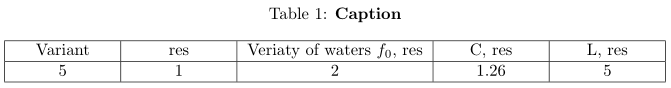
\includegraphics[width=1\linewidth]{4.5.png}
\textit{a command was also created to make a new cell view in the table}
}{4.4}
\end{minipage}
&
\begin{minipage}[m]{0.55\textwidth}
\renewcommand\textminus{\mbox{-}}%<<<<<<<<<<<
\begin{lstlisting}[numberstyle=\zebra{green!15}{yellow!15},numbers=left,basicstyle=\scriptsize]{tex}
\usepackage{graphicx}
\usepackage{tabularx}
\newcolumntype{Y}{>{\centering\arraybackslash}X}
\begin{document}
\begin{table}[h!]
\begin{center}
\caption{\textbf{Caption}}
  \begin{tabularx}{14cm}{|Y|Y|c|Y|Y|}
  \hline
  Variant & res & Veriaty of waters $f_0$, res & C, res & L, res\\
  \hline
  5       &     1   &               2               & 1.26 & 5\\
  \hline
  \end{tabularx}
\end{center}
\end{table}
\end{lstlisting}
\end{minipage}
\end{tabular}
\end{table}
\clearpage

%#################### 4.5 ####################
\section{bclogo – Creating colourful boxes with logos}
\begin{table}[h!]
\begin{tabular}{c | c}
\begin{minipage}[m]{0.4\textwidth}
\enum{\href{https://ctan.org/pkg/bclogo}{\img{1}{images/4.5/4.5.pdf}}}{4.5}
\end{minipage}
&
\begin{minipage}[m]{0.55\textwidth}
\renewcommand\textminus{\mbox{-}}%<<<<<<<<<<<
\begin{lstlisting}[numberstyle=\zebra{green!15}{yellow!15},numbers=left,basicstyle=\scriptsize]
\documentclass{article}
\usepackage{geometry}
\geometry{
paperwidth=8cm,
paperheight=14cm,
margin=0.5cm
}
\usepackage{xcolor}
\usepackage[most]{tcolorbox}
\usepackage[tikz]{bclogo}

\newtcolorbox{framedd}[1][]{
  colframe=lightgray,
  colback=yellow!40!white,
  enhanced jigsaw,
  sharp corners,
  lower separated=false,
  lefthand width=1cm,
  sidebyside gap=0.5cm,
  sidebyside,#1}

\begin{document}
\begin{framedd}
  \bcbombe  \tcblower  Some text inside.
\end{framedd}

\begin{framedd}[colback=blue!40!green]
  \bclampe   \tcblower  Some text inside.
\end{framedd} 

\begin{framedd}
  \bcattention  \bcinterdit  \tcblower
  Some text inside.
\end{framedd}

\begin{framedd}[colback=blue!40!green]
   \bcnucleaire  \tcblower
  Some text inside.
\end{framedd}

\begin{framedd}[colback=blue!40!green]
 \bcdanger \tcblower
  Some text inside.
\end{framedd}

\begin{framedd}
  \bcquestion \tcblower
  Some text inside.
\end{framedd}

\begin{framedd}[colback=blue!40!green, lefthand width=2.5cm]
  \bcsoleil  \bceclaircie \bcpluie  \bcneige \tcblower
  Some text inside.
\end{framedd}

\begin{framedd}[lefthand width=3cm]
  \bccube \bcdodecaedre \bcicosaedre \bcoctaedre \bctetraedre  \tcblower
  Some text inside.
\end{framedd}
\end{document}
\end{lstlisting}
\end{minipage}
\end{tabular}
\end{table}

  
\clearpage
%#################### 4.6 ####################
\section{Warning banner}
\begin{tabular}{c | c}
\begin{minipage}[m]{0.4\textwidth}
\enum{
\begin{caja}[title=warning]
Here is some text 
\end{caja}}{4.6}
\end{minipage}
&
\begin{minipage}[m]{0.55\textwidth}
\renewcommand\textminus{\mbox{-}}%<<<<<<<<<<<
\begin{lstlisting}[numberstyle=\zebra{green!15}{yellow!15},numbers=left,basicstyle=\footnotesize]{tex}
\usepackage[utf8]{inputenc}
\usepackage[T1]{fontenc}
\usepackage[most]{tcolorbox}
\definecolor{orang}{RGB}{255,155,0}
\newtcolorbox[auto counter,number within=section]{caja}[1][]{
enhanced jigsaw,colback=white,colframe=orang,coltitle=orang,
fonttitle=\bfseries\sffamily,
sharp corners,
detach title,
leftrule=10mm,
% What you need %%%%%%%%%%%%
underlay unbroken and first={\node[below,text=black,anchor=east]
at ([xshift=-5.5pt]interior.base west) {\Huge  \textbf{!}};},
%%%%%%%%%%%%%%%%%%%%%%%%
breakable,pad at break=1mm,
#1,
code={\ifdefempty{\tcbtitletext}{}{\tcbset{before upper={\tcbtitle\par\medskip}}}},}
\begin{document}
\begin{caja}[title=warning]
The vertical alignment settings 
\end{caja}
\end{document}	
\end{lstlisting}
\end{minipage}
\end{tabular}

\vspace{0.2cm}	

%#################### 4.7 ####################
\section{Photo positioning}
\begin{tabular}{c | c}
\begin{minipage}[m]{0.4\textwidth}
\enum{
\begin{tcolorbox}[enhanced,sharp corners,
width={5cm},
colback=white,
overlay={\node at (frame.south east) {\includegraphics[scale=0.1]{example-image-a}};} ]
Sample text here.
\end{tcolorbox}}{4.7}
\end{minipage}
&
\begin{minipage}[m]{0.55\textwidth}
\renewcommand\textminus{\mbox{-}}%<<<<<<<<<<<
\begin{lstlisting}[numberstyle=\zebra{green!15}{yellow!15},numbers=left,basicstyle=\footnotesize]{tex}
\documentclass{article}
\usepackage[most]{tcolorbox}
\usepackage{graphicx}
\begin{document}
\begin{tcolorbox}[enhanced,sharp corners,
width={5cm},
colback=white,
overlay={\node at (frame.south east) {\includegraphics[scale=0.1]{example-image-a}};} ]
Sample text here.
\end{tcolorbox}
\end{document}	
\end{lstlisting}
\end{minipage}
\end{tabular}

%#################### 4.8 ####################
\section{Absolutely centered cells (vertically and horisontally)}
\begin{tabular}{c | c}
\begin{minipage}[m]{0.4\textwidth}
\enum{

 
\makegapedcells
    \begin{tabular}{|c|c|c| }
    \hline
all&in&cells\\ \hline
are&centered&vertically\\ \hline
and&horisontally&$\sum$\\ \hline
 
\end{tabular}
 
 }{4.8}
\end{minipage}
&
\begin{minipage}[m]{0.55\textwidth}
\renewcommand\textminus{\mbox{-}}%<<<<<<<<<<<
\begin{lstlisting}[numberstyle=\zebra{green!15}{yellow!15},numbers=left,basicstyle=\footnotesize]{tex}
\documentclass{article}
\usepackage{float}
\usepackage{array, makecell}
\setcellgapes{5pt}

\begin{document}
\begin{table}[H]
\center
\makegapedcells
    \begin{tabular}{|c|c|c|c|}
    \hline
1&1&1&1\\ \hline
1&1&1&1\\ \hline
1&1&1&1\\ \hline
 
\end{tabular}
\end{table}

\end{document}
\end{lstlisting}
\end{minipage}
\end{tabular}

%#################### 4.9 ####################
\section{Martix made of table}
\begin{tabular}{c | c}

\begin{minipage}[m]{0.4\textwidth}
\enum{    
 
\begin{tabular}{l|l c r|l}
 
        & $a_{1,1}$ & $\dots, a_{1,n}$ & 0 &                 \\  
        & $a_{1,1}$ & $\dots, a_{1,n}$ & 0 &                 \\ 
        & \multicolumn{3}{l|}{\dotfill}   &                  \\  
        & $a_{1,1}$ & $\dots, a_{1,n}$ & 0 &                 \\ 
$d_{n+1}$ &         &                &   & = 0 \\  
        & $a_{1,1}$ & $\dots, a_{1,n}$ & 0 &                 \\  
        & $a_{1,1}$ & $\dots, a_{1,n}$ & 0 &                 \\ 
        & \multicolumn{3}{l|}{\dotfill}   &                  \\ 
        & $a_{1,1}$ & $\dots, a_{1,n}$ & 0 &                 \\ 
\end{tabular}
 }{4.9}

\end{minipage}
&
\begin{minipage}[m]{0.55\textwidth}
\renewcommand\textminus{\mbox{-}}%<<<<<<<<<<<
\begin{lstlisting}[numberstyle=\zebra{green!15}{yellow!15},numbers=left,basicstyle=\footnotesize]{tex}
\documentclass[a4paper,14pt]{extreport}
\begin{document}
\begin{table}[]
\begin{tabular}{l|l c r|l}
& $a_{1,1}$ & $\dots, a_{1,n}$ & 0 &                 \\  
& $a_{1,1}$ & $\dots, a_{1,n}$ & 0 &                 \\ 
& \multicolumn{3}{l|}{\dotfill}   &                  \\  
& $a_{1,1}$ & $\dots, a_{1,n}$ & 0 &                 \\ 
$d_{n+1}$ &         &    &   & = $\pm 2ad_n$ = 0     \\  
& $a_{1,1}$ & $\dots, a_{1,n}$ & 0 &                 \\  
& $a_{1,1}$ & $\dots, a_{1,n}$ & 0 &                 \\ 
& \multicolumn{3}{l|}{\dotfill}   &                  \\ 
& $a_{1,1}$ & $\dots, a_{1,n}$ & 0 &                 \\ 
\end{tabular}
\end{table}
\end{document}
\end{lstlisting}
\end{minipage}
\end{tabular}

%#################### 4.10 ####################
\section{Centering cells with \xmybox{NiceTabular}}
\begin{tabular}{c | c}
\begin{minipage}[m]{0.4\textwidth}
\enum{ \begin{NiceTabular}{|c|c|c|} 
\hline
\cellcolor{red}1& \cellcolor{green}1 & \cellcolor{black!10}EVERY\\\hline 
\cellcolor{orange}1 & \cellcolor{red!35}1 & \cellcolor{brown!50}CELL \\ \hline
\cellcolor{green!35}1 & \cellcolor{blue!45}1 & \cellcolor{yellow}CENTERED \\ \hline
\end{NiceTabular}  }{4.10}
\end{minipage}
&
\begin{minipage}[m]{0.55\textwidth}
\renewcommand\textminus{\mbox{-}}%<<<<<<<<<<<
\begin{lstlisting}[numberstyle=\zebra{green!15}{yellow!15},numbers=left,basicstyle=\footnotesize] 
\documentclass{article}
\usepackage[table]{xcolor}
\usepackage{nicematrix}
\NiceMatrixOptions{cell-space-top-limit=5pt,cell-space-bottom-limit=5pt}

\begin{document}
\begin{table}[htbp]
\centering
\begin{NiceTabular}{|c|c|c|} 
\hline
\cellcolor{red}1& \cellcolor{green}1 &  1 \\ \hline 
\cellcolor{orange}1 & \cellcolor{red!35}1 &  1 \\ \hline
\cellcolor{green!35}1 & \cellcolor{blue!45}1 &  1 \\ \hline
\end{NiceTabular}
\end{table}
\end{document}
\end{lstlisting}
\end{minipage}
\end{tabular}


%#################### 4.11 ####################
\section{Centered cells in \xmybox{longtable}}
\begin{tabular}{c | c}
\begin{minipage}[m]{0.4\textwidth}
\enum{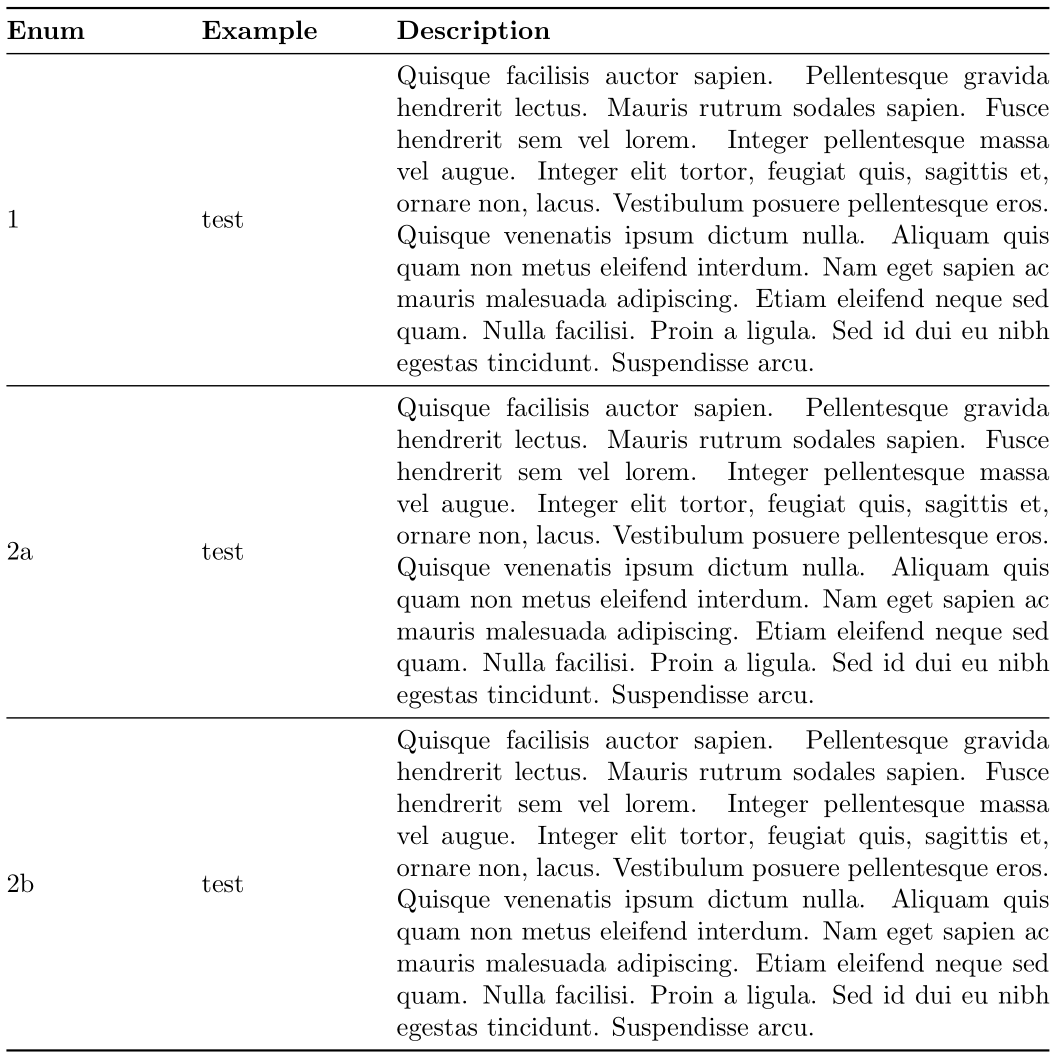
\includegraphics[width=1.\linewidth]{4.11.png}}{4.11}
\end{minipage}
&
\begin{minipage}[m]{0.55\textwidth}
\renewcommand\textminus{\mbox{-}}%<<<<<<<<<<<
\begin{lstlisting}[numberstyle=\zebra{green!15}{yellow!15},numbers=left,basicstyle=\footnotesize] 
\documentclass{article}
\usepackage[left=1.5cm,right=1.5cm,
top=1.5cm,bottom=2cm,bindingoffset=0cm]{geometry}
\usepackage{float}
\usepackage{array, makecell}
\usepackage[utf8]{inputenc}
\usepackage{lipsum}
\usepackage{booktabs}
\usepackage{multirow}
\usepackage{pdflscape}
\usepackage{longtable, array}

\begin{document}
\begin{landscape}
\begin{longtable}{@{} *{2}{m{.15\paperwidth}} *{1}{m{.40\paperwidth}} @{}}
\endfirsthead
\endhead
\toprule
\textbf{Enum} & \textbf{Example} & \textbf{Description} \\
\midrule
1 & test & \lipsum[50]\\
\midrule
2a & test & \lipsum[50]\\
2b & test & \lipsum[50]\\
\bottomrule
\end{longtable}
\end{landscape}
\end{document}          
\end{lstlisting}
\end{minipage}
\end{tabular}

%#################### 4.12 ####################
\section{If table is not wide enough}
\begin{tabular}{c | c}
\begin{minipage}[m]{0.4\textwidth}
\enum{ 
\begin{tabularx}{\textwidth}{X  X  X  X}
       & Item1 & Item2 & Item3 \\ \midrule
Group1 & 0.8   & 0.1   & 0.1  \\
Group2 & 0.1   & 0.8   & 0.1  \\
Group3 & 0.1   & 0.1   & 0.8  \\
Group4 & 0.34  & 0.33  & 0.33 \\ \bottomrule
\end{tabularx}}{4.12}
\end{minipage}
&
\begin{minipage}[m]{0.55\textwidth}
\renewcommand\textminus{\mbox{-}}%<<<<<<<<<<<
\begin{lstlisting}[numberstyle=\zebra{green!15}{yellow!15},numbers=left,basicstyle=\footnotesize] 
\documentclass{article}
\usepackage[left=1.5cm,right=1.5cm,
top=1.5cm,bottom=2cm,bindingoffset=0cm]{geometry}
\usepackage{graphicx}
\usepackage{booktabs}
\usepackage{tabularx}

\begin{document}
           
\begin{table}[!ht] 
\caption{Vertical and lateral stresses of mortar.}  
\vspace{0.5cm}
\begin{tabularx}{\textwidth}{X  X  X  X}
       & Item1 & Item2 & Item3 \\ \midrule
Group1 & 0.8   & 0.1   & 0.1  \\
Group2 & 0.1   & 0.8   & 0.1  \\
Group3 & 0.1   & 0.1   & 0.8  \\
Group4 & 0.34  & 0.33  & 0.33 \\ \bottomrule
\end{tabularx}
\label{c}
\end{table}

\end{document}        
\end{lstlisting}
\end{minipage}
\end{tabular}


%#################### 4.13 ####################
\section{Text next to a table}
\begin{tabular}{c | c}
\begin{minipage}[m]{0.4\textwidth}
\enum{\begin{minipage}[m]{0.4\textwidth}
text  text text
\end{minipage}
\hfill
\begin{minipage}[m]{0.5\textwidth}
\begin{tabular}{|c|c|c|}
\hline
1 & 22 & 333  \\ \hline
  &    &      \\ \hline
  &    &      \\ \hline
  &    &      \\ \hline
\end{tabular}
\end{minipage}}{4.13}
\end{minipage}
&
\begin{minipage}[m]{0.55\textwidth}
\renewcommand\textminus{\mbox{-}}%<<<<<<<<<<<
\begin{lstlisting}[numberstyle=\zebra{green!15}{yellow!15},numbers=left,basicstyle=\footnotesize] 
\documentclass[a4paper,14pt]{extreport}
\usepackage[left=1.5cm,right=1.5cm,top=1.5cm,bottom=2cm,bindingoffset=0cm]{geometry}
\usepackage{lipsum}

\begin{document}
\begin{minipage}[m]{0.58\textwidth}
text text text
\end{minipage}
\hspace{0.2cm}
\begin{minipage}[m]{0.40\textwidth}
\begin{tabular}{|c|c|c|}
\hline
1 & 22 & 333 &  \\ \hline
  &    &     &  \\ \hline
  &    &     &  \\ \hline
  &    &     &  \\ \hline
\end{tabular}
\end{minipage}
\end{document}
\end{lstlisting}
\end{minipage}
\end{tabular}

%#################### 4.14 ####################
\section{Text next to a table}
\begin{tabular}{c | c}
\begin{minipage}[m]{0.4\textwidth}
\enum{  \center \begin{tikzpicture}[
    start chain=going below,
    node distance=2mm,
    Node/.style = {minimum width=#1,
                   shape=rectangle, 
                   draw, fill=white,
                   on chain},
    Pattern/.style = {pattern=north east hatch,
                    pattern color=teal!30,
                    hatch distance=7pt, 
                    hatch thickness=2pt},
    font=\small\sffamily]
%----------------
    \node[Node=24mm, Pattern, 
            preaction={fill=white}] (a) {without shadow};
    \begin{scope}[on background layer]
        \node[fit=(a),fill=red] {};
    \end{scope}

    \node[Node=24mm, drop shadow,
            preaction={fill=yellow}, Pattern] (b) {with shadow};

    \node[Node=24mm, preaction={fill=yellow},
            drop shadow, Pattern] (b) {with shadow};

    \node[Node=24mm, postaction={Pattern},
            drop shadow] (b) {with shadow};

    \node[Node=24mm, postaction={draw=red, Pattern},
            drop shadow] (b) {with shadow};

    \node[Node=24mm, drop shadow] (c) {without pattern};

   
%---
 \end{tikzpicture} 
  \href{https://tex.stackexchange.com/questions/154842/using-pattern-inside-tikz-shapes-with-dropped-shadows}{*****} }{4.14}
\end{minipage}
&
\begin{minipage}[m]{0.55\textwidth}
\renewcommand\textminus{\mbox{-}}%<<<<<<<<<<<
\begin{lstlisting}[numberstyle=\zebra{green!15}{yellow!15},numbers=left,basicstyle=\scriptsize] 
\documentclass[tikz,border=5mm]{standalone}
\usetikzlibrary{chains,patterns,shadows,fit,backgrounds}

\makeatletter
\tikzset{% customization of pattern
         % based on <m.wibrow@gm...> - 2013-03-24 07:20: 
        hatch distance/.store in=\hatchdistance,
        hatch distance=5pt,
        hatch thickness/.store in=\hatchthickness,
        hatch thickness=5pt
        }
\pgfdeclarepatternformonly[\hatchdistance,\hatchthickness]{north east hatch}% name
    {\pgfqpoint{-1pt}{-1pt}}% below left
    {\pgfqpoint{\hatchdistance}{\hatchdistance}}% above right
    {\pgfpoint{\hatchdistance-1pt}{\hatchdistance-1pt}}%
    {
        \pgfsetcolor{\tikz@pattern@color}
        \pgfsetlinewidth{\hatchthickness}
        \pgfpathmoveto{\pgfqpoint{0pt}{0pt}}
        \pgfpathlineto{\pgfqpoint{\hatchdistance}{\hatchdistance}}
        \pgfusepath{stroke}
    }
\makeatother

\begin{document}
 \begin{tikzpicture}[
    start chain=going below,
    node distance=2mm,
    Node/.style = {minimum width=#1,
                   shape=rectangle, 
                   draw, fill=white,
                   on chain},
    Pattern/.style = {pattern=north east hatch,
                    pattern color=teal!30,
                    hatch distance=7pt, 
                    hatch thickness=2pt},
    font=\small\sffamily]
%----------------
    \node[Node=24mm, Pattern, 
            preaction={fill=white}] (a) {without shadow};
    \begin{scope}[on background layer]
        \node[fit=(a),fill=red] {};
    \end{scope}

    \node[Node=24mm, drop shadow,
            preaction={fill=yellow}, Pattern] (b) {with shadow};

    \node[Node=24mm, preaction={fill=yellow},
            drop shadow, Pattern] (b) {with shadow};

    \node[Node=24mm, postaction={Pattern},
            drop shadow] (b) {with shadow};

    \node[Node=24mm, postaction={draw=red, Pattern},
            drop shadow] (b) {with shadow};

    \node[Node=24mm, drop shadow] (c) {without pattern};
%---
 \end{tikzpicture}   
\end{document}
\end{lstlisting}
\end{minipage}
\end{tabular}


%#################### 4.15 ####################
\section{Hand Drawn tcolorbox}
\begin{tabular}{c | c}
\begin{minipage}[m]{0.4\textwidth}
\enum{\begin{mytheo}{}{theoexample}
some text
\end{mytheo}}{4.15}
\end{minipage}
&
\begin{minipage}[m]{0.55\textwidth}
\renewcommand\textminus{\mbox{-}}%<<<<<<<<<<<
\begin{lstlisting}[numberstyle=\zebra{green!15}{yellow!15},numbers=left,basicstyle=\footnotesize] 
\documentclass{article}
\usepackage[most]{tcolorbox}
\usepackage{emerald}
\usetikzlibrary{decorations.pathmorphing}
\usetikzlibrary{shadows}
\tikzset{decoration={random steps,segment length=2mm,amplitude=0.6pt}}
\newtcbtheorem{mytheo}{Theorem}{
  coltitle=green!80!black,
  colback=lightgray!20,
  colbacktitle=lightgray!20,
  fonttitle=\bfseries\ECFAugie,
  enhanced,
  attach boxed title to top left={yshift=-0.18cm,xshift=-0.5mm},
  boxed title style={
    tikz={rotate=4,transform shape},
    frame code={
      \draw[decorate,fill=lightgray!20] (frame.south west) rectangle (frame.north east);
    }  },
  frame code={
    \draw[decorate,fill=lightgray!20,drop shadow] (frame.north east) rectangle (frame.south west);
  },}{th}

\begin{document}
\begin{mytheo}{}{theoexample}
content...
\end{mytheo}
\end{document}
\end{lstlisting}
\end{minipage}
\end{tabular}


%#################### 4.16 ####################%https://tex.stackexchange.com/questions/624558/how-can-i-do-this-block-in-beamer
\section{Halfframed boxes}
\begin{tabular}{c | c}
\begin{minipage}[m]{0.4\textwidth}
\enum{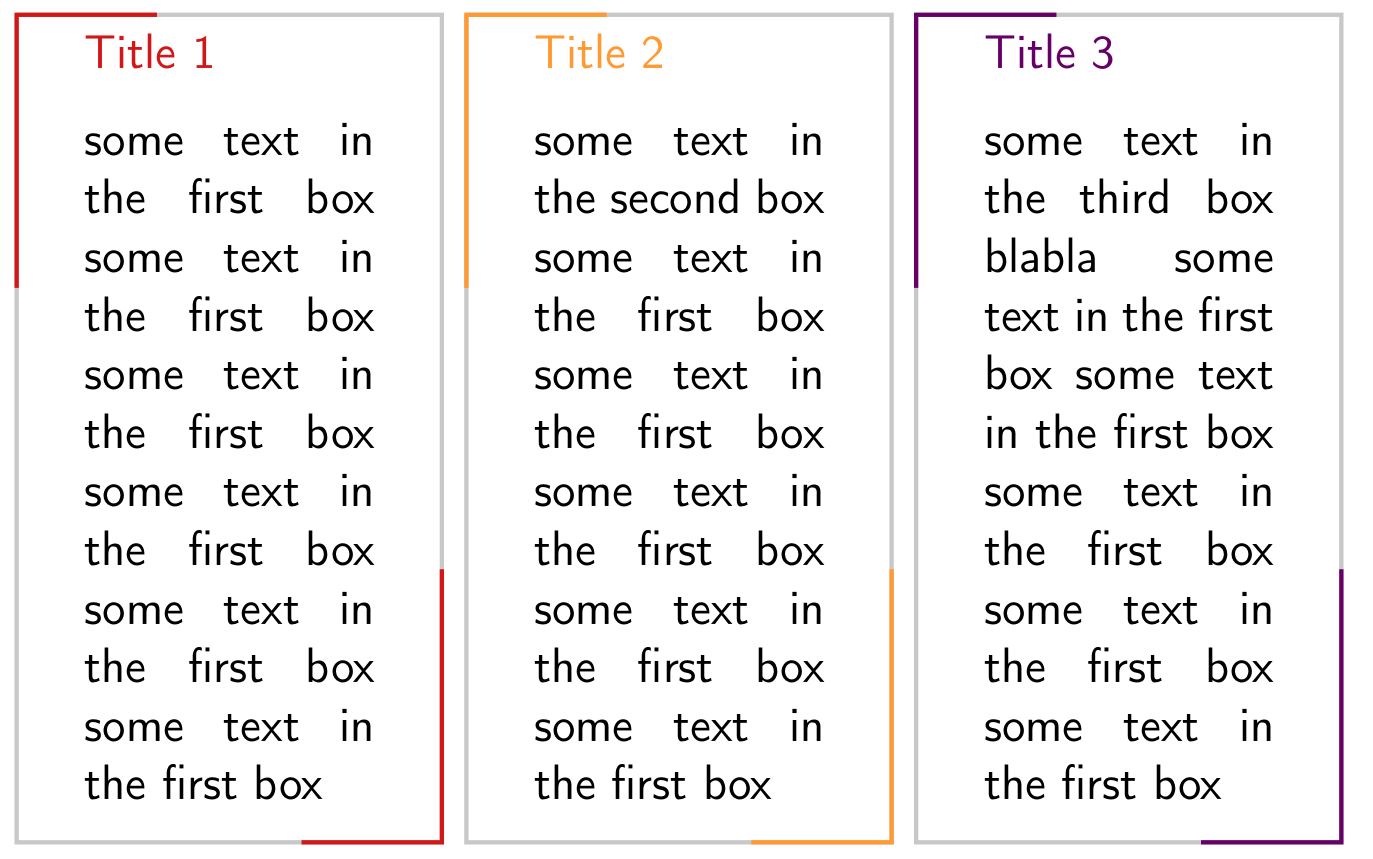
\includegraphics[width=1\linewidth]{4.16.png}}{4.16}
\end{minipage}
&
\begin{minipage}[m]{0.55\textwidth}
\renewcommand\textminus{\mbox{-}}%<<<<<<<<<<<
\begin{lstlisting}[numberstyle=\zebra{green!15}{yellow!15},numbers=left,basicstyle=\footnotesize] 
\documentclass{beamer}
\usepackage[english]{babel}
\usepackage[T1]{fontenc}
\usepackage[utf8]{inputenc}
\usepackage{tikz}
\usepackage{tcolorbox}
\usetikzlibrary{calc}
\tcbuselibrary{skins,breakable,raster}
\makeatletter
\definecolor{myred}{RGB}{209,23,23}
\definecolor{myorange}{RGB}{255,153,51}
\definecolor{mypurple}{RGB}{102,0,102}
\definecolor{mygrey}{RGB}{200,200,200}

\newtcolorbox{mybox}[2]{%
empty,
coltitle = #1,
title = #2,
overlay ={
\draw[mygrey,line width=1pt]
(frame.north west)--(frame.north east)--(frame.south east)--(frame.south west)--(frame.north west);
\draw[#1,line width=1pt]
($(frame.north west)!0.33!(frame.south west)$)
--(frame.north west)
--($(frame.north west)!0.33!(frame.north east)$);
\draw[#1,line width=1pt]
($(frame.south east)!0.33!(frame.south west)$)
--(frame.south east)
--($(frame.south east)!0.33!(frame.north east)$);}}

\tcbset{marktext/.style={%
  overlay={\node[rotate=90,text=black,anchor=north east] at (frame.north west){#1};},
  code={\setbox\z@=\color@hbox#1\color@endbox\tcbdimto\myheight{\wd\z@+3mm}},
  minimum for equal height group=\tcb@ehgid:\myheight,  }}
\makeatother

\begin{document}
\begin{frame}
\begin{tcbraster}[%
    raster columns=3,
    raster equal height=rows
    ]
    \begin{mybox}{myred}{Title 1}
    some text in the first box
    \end{mybox}
    \begin{mybox}{myorange}{Title 2}
    some text in the second box
    \end{mybox}
    \begin{mybox}{mypurple}{Title 3}
    some text in the third box blabla
    \end{mybox}
\end{tcbraster}
\end{frame}
\end{document}
\end{lstlisting}
\end{minipage}
\end{tabular}
%#################### 4.17 ####################
%#################### 4.18 ####################
%#################### 4.19 ####################










 
 


%------------------C5-Figures
\chapter{Figures}



-------------------------------------------- 5.1 --------------------------------------------
\begin{table}[h!]
\begin{tabular}{c | c}
\begin{minipage}[m]{0.4\textwidth}
\begin{tikzpicture}
        \node [anchor=south west] at (0, 0) (cartoon) {\includegraphics[width=.15\textwidth,height=.15\textwidth]{example-image-a}};
        \node [anchor=north west,rectangle callout,draw=black,
        callout absolute pointer=(cartoon.east), 
        rounded corners=3pt,text width=0.7\textwidth, inner sep=2ex] at (.19\textwidth,.125\textwidth) {This is an example.};
    \end{tikzpicture}
\end{minipage}
&
\begin{minipage}[m]{0.55\textwidth}
\begin{lstlisting}[basicstyle=\footnotesize]
\usepackage{tikz}
\usepackage[framemethod=TikZ]{mdframed}
\usepackage{xcolor}
\usetikzlibrary{calc}
\makeatletter
\newlength{\mylength}
\xdef\CircleFactor{1.1}
\setlength\mylength{\dimexpr\f@size pt}
\newsavebox{\mybox}
\newcommand*\circled[2][draw=blue]{\savebox\mybox{\vbox{\vphantom{WL1/}#1}}\setlength\mylength{\dimexpr\CircleFactor\dimexpr\ht\mybox+\dp\mybox\relax\relax}\tikzset{mystyle/.style={circle,#1,minimum height={\mylength}}}
\tikz[baseline=(char.base)]
\node[mystyle] (char) {#2};}
\makeatother
\definecolor{amber}{rgb}{1.0, 0.75, 0.0}
\definecolor{babyblue}{rgb}{0.54, 0.81, 0.94}	
\end{lstlisting}
\end{minipage}
\end{tabular}
\end{table}

%-------------------5.2
-------------------------------------------- 5.2 --------------------------------------------
\begin{table}[h!]
\begin{tabular}{c | c}
\begin{minipage}[m]{0.4\textwidth}
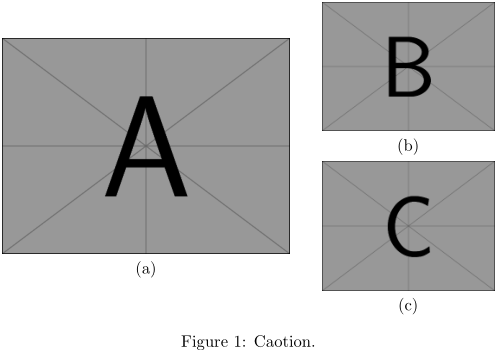
\includegraphics[width=1\linewidth]{5.2.png}
\end{minipage}
&
\begin{minipage}[m]{0.55\textwidth}
\begin{lstlisting}[basicstyle=\footnotesize]
\documentclass{article}
\usepackage{graphicx}
\usepackage{subfig}
\begin{document}
\begin{figure}[htp]
\centering
\begin{tabular}{@{}c@{}}
\subfloat{\includegraphics[width=0.5\linewidth]{example-image-a.png}}\\ (a)
\end{tabular}\qquad % some space
\begin{tabular}{@{}c@{}}
\subfloat{\includegraphics[width=0.3\linewidth]{example-image-b.png}}\\ (b)
\\[0.1cm]
\subfloat{\includegraphics[width=0.3\linewidth]{example-image-c.png}}\\ (c)
\end{tabular}
\caption{Caption.}
\end{figure}
\end{document}
\end{lstlisting}
\end{minipage}
\end{tabular}
\end{table}

\newpage
-------------------------------------------- 5.3 --------------------------------------------
\begin{table}[ht!]
\begin{tabular}{c | c}
\begin{minipage}[m]{0.4\textwidth}
 \begin{tikzpicture}
\node[ above left,
      xshift=5cm, %shifting around
      yshift=-3cm]  
{\includegraphics[width=3cm]{example-image-a.png}};
  % define destination coordinates
  \path (5,-3) coordinate (anode);
\end{tikzpicture}

\end{minipage}
&
\begin{minipage}[m]{0.55\textwidth}
\begin{lstlisting}[basicstyle=\footnotesize]
\usepackage{graphicx}
\usepackage{tikz}
\begin{document}
\begin{tikzpicture}[overlay, remember picture]
\node[anchor=north west,xshift=4cm,yshift=-11cm]
at (current page.north west) 
{\includegraphics[width=5.5cm]{example-image-a.png}};
\end{tikzpicture}
\end{document}
\end{lstlisting}
\tikz[na] \coordinate (s-anode); \xmybox[red!70!white]{place image anywhere You want}
\end{minipage}
\end{tabular}
\end{table}
\begin{tikzpicture}[overlay]
\path[->,red,thick] (s-anode) edge [bend left] (anode);
\end{tikzpicture}
-------------------------------------------- 5.4 --------------------------------------------



%------------------C6
\chapter{Numbering, enumeration, itemizing}

	\begin{table}[h!]
	\begin{tabular}{c | c}
	\begin{minipage}[m]{0.4\textwidth}
	\begin{multicols}{2}%change it 2,3,4... 
	\begin{enumerate}
	\item c
	\item g
	\item d
	\item f
	\end{enumerate}
	\end{multicols}
	\end{minipage}
	&
	\begin{minipage}[m]{0.55\textwidth}
	\begin{lstlisting}[numberstyle=\zebra{blue!15}{orange!15},numbers=left,basicstyle=\footnotesize]{tex}
\usepackage{multicol} 
\begin{document}
\begin{multicols}{2}%change it 2,3,4... 
\begin{enumerate}
\item c
\item g
\item d
\item f
\end{enumerate}
\end{multicols}
\end{document}
	\end{lstlisting}
	\xmybox[green!70!white]{Numbering in few columns}
	\end{minipage}
	\end{tabular}
	\end{table}

-------------------------------------------- 6.1 --------------------------------------------



%------------------C7
\chapter{Plots, tikz, pie charts ...}
%#################### 7.1 ####################
\subsection{\hll{Simple pie chart}}

\begin{tabular}{c | c}
\begin{minipage}[m]{0.4\textwidth}
\enum{ 
\begin{tikzpicture}[thick,scale=0.6, every node/.style={transform shape}] 
\pie{22.97/Los Angeles Lakers,
22.97/Boston,
8.11/Golden State,
8.11/Chicago,
6.76/San ,
31.07/Other Teams}
\end{tikzpicture}}{\thesubsection}
\end{minipage}
&
\begin{minipage}[m]{0.55\textwidth}
\renewcommand\textminus{\mbox{-}}%<<<<<<<<<<<
\begin{lstlisting}[numberstyle=\zebra{red!15}{yellow!15},numbers=left,basicstyle=\ttfamily\footnotesize]{tex}
\documentclass[border=0.2cm]{standalone} 
\usepackage{pgf-pie}  

\begin{document}
\begin{tikzpicture}
\pie{22.97/Los Angeles Lakers,
22.97/Boston Celtics,
8.11/Golden State Warriors,
8.11/Chicago Bulls,
6.76/San Antonio Spurs,
31.07/Other Teams}
\end{tikzpicture}
\end{document}
\end{lstlisting}
\end{minipage}
\end{tabular}


	%#################### 7.2 ####################
\subsection{\hll{Circled arrows with text}}

\begin{tabular}{c | c}
\begin{minipage}[m]{0.4\textwidth}
\enum{ 
\begin{center}
\begin{tikzpicture}[->,scale=.9]
\node (i) at (90:1cm)  {$T$};
\node (j) at (-30:1cm) {$D$};
\node (k) at (210:1cm) {$R$};
\draw (70:1cm)  arc (70:-10:1cm) node[midway, right] {{\footnotesize 1}};
\draw (-50:1cm) arc (-50:-130:1cm) node[midway, below] {{\footnotesize 1}};
\draw (190:1cm) arc (190:110:1cm) node[midway, left] {{\footnotesize -1}};
\end{tikzpicture}\end{center}}{\thesubsection}
\end{minipage}
&
\begin{minipage}[m]{0.55\textwidth}
\renewcommand\textminus{\mbox{-}}%<<<<<<<<<<<
\begin{lstlisting}[numberstyle=\zebra{red!15}{yellow!15},numbers=left,basicstyle=\ttfamily\scriptsize]{tex}
\documentclass{article} 
\usepackage{tikz}

\begin{document}
\begin{tikzpicture}[->,scale=.7]
\node (i) at (90:1cm)  {$T$};
\node (j) at (-30:1cm) {$D$};
\node (k) at (210:1cm) {$R$};
\draw (70:1cm)  arc (70:-10:1cm) node[midway, right] {{\footnotesize 1}};
\draw (-50:1cm) arc (-50:-130:1cm) node[midway, below] {{\footnotesize 1}};
\draw (190:1cm) arc (190:110:1cm) node[midway, left] {{\footnotesize -1}};
\end{tikzpicture}
\end{document}
\end{lstlisting}
\end{minipage}
\end{tabular}

\newpage
%#################### 7.3 ####################
\subsection{\hll{Diamond with text}}
	
	\begin{tabular}{c | c}
	\begin{minipage}[m]{0.4\textwidth}
	\enum{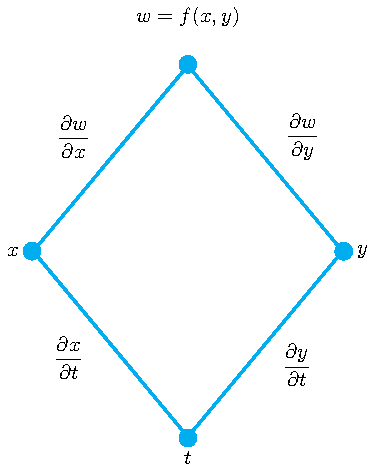
\includegraphics[width=1\linewidth]{7.3.pdf}}{\thesubsection}
	\end{minipage}
	&
	\begin{minipage}[m]{0.55\textwidth}
	\renewcommand\textminus{\mbox{-}}%<<<<<<<<<<<
	\begin{lstlisting}[numberstyle=\zebra{red!15}{yellow!15},numbers=left,basicstyle=\ttfamily\scriptsize]
\documentclass[a4paper,14pt]{extreport}
\usepackage[left=1.5cm,right=1.5cm,top=1.5cm,bottom=2cm,bindingoffset=0cm]{geometry}
\usepackage{amsmath}
\usepackage{tikz}
\usetikzlibrary{shapes.geometric}
 
\begin{document}
\begin{tikzpicture}
\node[diamond,font=\small,
line width=0.4mm,scale=0.7,
    draw = cyan, minimum width = 7.5cm, %text = red,
    minimum height = 9cm] (d) at (0,0) { };
      \node [above=0.5cm] (a) at (d.90) {$w = f(x,y)$};
      \node [above=0.5cm,right=0.1cm] (b) at (d.45) {$\dfrac{\partial w}{\partial y}$};
      \node [above=0.5cm,left=0.1cm] (c) at (d.135) {$\dfrac{\partial w}{\partial x}$};
      \node [left=0.1cm] (dd) at (d.180) {$x$};
      \node [right=0.1cm] (e) at (d.0) {$y$};
      \node [below=0.1cm] (f) at (d.270) {$t$};
      \node [below=0.9cm,right=-0.3cm] (g) at (d.-30) {$\dfrac{\partial y}{\partial t}$};
      \node [below=0.5cm,left=0.1cm] (h) at (d.220) {$\dfrac{\partial x}{\partial t}$};
      \node at (d.90) [cyan,circle,fill,inner sep=3pt]{};
      \node at (d.180) [cyan,circle,fill,inner sep=3pt]{};
      \node at (d.0) [cyan,circle,fill,inner sep=3pt]{};
      \node at (d.270) [cyan,circle,fill,inner sep=3pt]{};
\end{tikzpicture}
\end{document}
\end{lstlisting}
	\end{minipage}
	\end{tabular}
	



%#################### 7.4 ####################
\subsection{\hll{Levels of skills }}

\begin{tabular}{c | c}
\begin{minipage}[m]{0.4\textwidth}
\enum{   
\skills{{Word/1}}\\
\skills{{\LaTeX/6}}\\
\skills{{C++/2}}\\
\skills{{Python/3}}\\
}{\thesubsection}
\end{minipage}
&
\begin{minipage}[m]{0.55\textwidth}
\renewcommand\textminus{\mbox{-}}%<<<<<<<<<<<
\begin{lstlisting}[numberstyle=\zebra{red!15}{yellow!15},numbers=left,basicstyle=\ttfamily\scriptsize]{tex}
\documentclass{report}
\usepackage[T1]{fontenc}
\usepackage{tikz}
\usepackage{xcolor}

\definecolor{white}{RGB}{255,255,255}
\definecolor{gray}{HTML}{4D4D4D}
\definecolor{maingray}{HTML}{B9B9B9}

\newcommand\skills[1]{ 
    \begin{tikzpicture}
        \foreach [count=\i] \x/\y in {#1}{
            \draw[fill=maingray,maingray] (0,\i) rectangle (6,\i+0.4);
            \draw[fill=white,gray](0,\i) rectangle (\y,\i+0.4);
            \node[above right] at (0,\i+0.4) {\x};
        }
    \end{tikzpicture}
}

\begin{document}
\skills{{b/2}}
\skills{{a/1}}
\end{document}
\end{lstlisting}
\end{minipage}
\end{tabular}


%#################### 7.5 ####################
\subsection{\hll{Round levels of skills }}

\begin{tabular}{c | c}
\begin{minipage}[m]{0.4\textwidth}
\enum{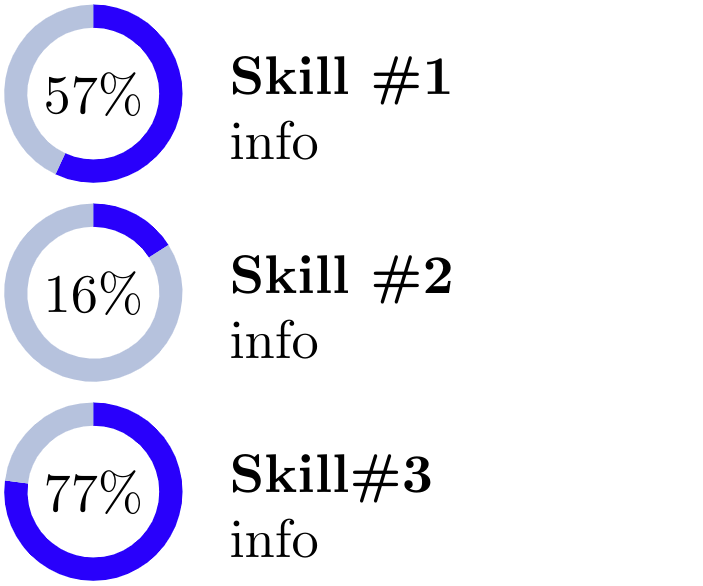
\includegraphics[width=1\linewidth]{7.5.png}}{\thesubsection}
\end{minipage}
&
\begin{minipage}[m]{0.55\textwidth}
\renewcommand\textminus{\mbox{-}}%<<<<<<<<<<<
\begin{lstlisting}[numberstyle=\zebra{red!15}{yellow!15},numbers=left,basicstyle=\ttfamily\scriptsize]{tex}
\documentclass[svgnames]{article}
\usepackage{tikz}
\usetikzlibrary{calc}
\usepackage{siunitx}% only to force percentages to be integers
\usepackage{enumitem}

\let\realItem\item% save for later use
\newcommand\percentageItem[1][10]{%
  \realItem[\smash{\tikz[baseline];
    \draw[thick,line width=1.5mm,Blue](90:5mm)
          arc [radius=5mm, start angle=90, delta angle=-#1*3.6];
    \draw[thick,line width=1.5mm,LightSteelBlue](90-#1*3.6:5mm)
          arc [radius=5mm, start angle=90-#1*3.6, end angle=-270];
    }}]%
}
\newlist{achievements}{itemize}{1}
\setlist[achievements]{
  before=\let\item\percentageItem,%make \item = \percentageItem
  leftmargin=*,
  label={},
  itemsep=3mm,
}

\begin{document}

\begin{achievements}
  \item[57]\textbf{Skill \#1}\\info
  \item[16]\textbf{Skill \#2}\\info
  \item[77]\textbf{Skill \#3}\\info
\end{achievements}

\end{document}
\end{lstlisting}
\end{minipage}
\end{tabular}

%#################### 7.6 ####################
\subsection{\hll{Huge margin line}}

\begin{tabular}{c | c}
\begin{minipage}[m]{0.4\textwidth}
\enum{
\includegraphics[width=0.85\linewidth]{7.6.png}}{\thesubsection}
\end{minipage}
&
\begin{minipage}[m]{0.55\textwidth}
\renewcommand\textminus{\mbox{-}}%<<<<<<<<<<<
\begin{lstlisting}[numberstyle=\zebra{red!15}{yellow!15},numbers=left,basicstyle=\ttfamily\scriptsize]{tex}
\documentclass{article}
\usepackage[margin=3cm]{geometry}
\usepackage{tikz}

\begin{document}
\tikz[overlay, remember picture] \draw[line width=2.5mm] ([xshift=1cm, yshift=-1cm]current page.north west) rectangle ([xshift=-1cm, yshift=1cm]current page.south east);
Text
\vfill
Text
\vfill
Text
\end{document}
\end{lstlisting}
\end{minipage}
\end{tabular}

\newpage
%#################### 7.7 ####################
\subsection{\hll{Aligning anything to a corer}}
\begin{tikzpicture}[remember picture,overlay]
\node[anchor=north east,yshift=0pt,xshift=0pt]%
at (current page.north east)
{\qrcode[height=1.cm]{https://github.com/AnMnv/eBook}% <--- put anything here
};
\end{tikzpicture}

\begin{tabular}{c | c}
\begin{minipage}[m]{0.4\textwidth}
\enum{\center Find me}{\thesubsection}
\end{minipage}
&
\begin{minipage}[m]{0.55\textwidth}
\renewcommand\textminus{\mbox{-}}%<<<<<<<<<<<
\begin{lstlisting}[numberstyle=\zebra{red!15}{yellow!15},numbers=left,basicstyle=\scriptsize]
\documentclass[14pt]{extreport}
\usepackage{tikz}
\usepackage{qrcode}

\begin{document}
\begin{tikzpicture}[remember picture,overlay]
\node[anchor=north west,yshift=0pt,xshift=0pt]%
at (current page.north west)
{\qrcode[height=0.5cm]{https://github.com/AnMnv/eBook}% <--- put here anything
};
\end{tikzpicture}
\end{document}

			OR the rainbow variant (see example 9.7)

\begin{tikzpicture}[remember picture,overlay]
\node at ($(current page.north west)+(.70cm,-.75cm)$) 
    {\fadingtext[scale=0.5]{path picture shading=rainbow}
    {\qrcode[height=3cm]{https://github.com/AnMnv/eBook}}};
\end{tikzpicture}
\end{lstlisting}
\end{minipage}
\end{tabular}

%#################### 7.8 ####################
\subsection{\hll{Family tree}}
\begin{tikzpicture}[remember picture,overlay]
\node[anchor=north east,yshift=0pt,xshift=0pt]%
at (current page.north east)
{\qrcode[height=1.cm]{https://github.com/AnMnv/eBook}% <--- put here anything
};
\end{tikzpicture}

\begin{tabular}{c | c}
\begin{minipage}[m]{0.4\textwidth}
\enum{\begin{tikzpicture}[scale=0.5, every node/.style={scale=0.5},level 1/.style={sibling distance=5cm},level 2/.style={sibling distance=2.5cm}]
	\node {My Family Tree}[edge from parent fork down]
		child { node {Uncle  - Aunty }}
		child { node {Mum - Dad}
			child {node{Me}}
			child {node{My sister}}
			}	
		child { node { Tom -  Sue}
			 child {node{ Josh}}
			 child {node{ Sarah}}
			};
\end{tikzpicture}

\vspace{1.0cm}

\begin{tikzpicture}[scale=0.5, every node/.style={scale=0.5},rotate=180,level 1/.style={sibling distance=5cm},level 2/.style={sibling distance=2.5cm}]
	\node {My Family Tree}[edge from parent fork down]
		child { node {Uncle  -  Jane}}
		child { node {Mum - Dad}
			child {node{Me}}
			child {node{sister}}
			}	
		child { node {Uncle  -  Sue}
			 child {node{ Josh}}
			 child {node{ Sarah}}
			};
\end{tikzpicture}}{\thesubsection}
\end{minipage}
&
\begin{minipage}[m]{0.55\textwidth}
\renewcommand\textminus{\mbox{-}}%<<<<<<<<<<<
\begin{lstlisting}[numberstyle=\zebra{red!15}{yellow!15},numbers=left,basicstyle=\ttfamily\scriptsize]
\documentclass{article}
\usepackage{tikz}
\usetikzlibrary{trees}

\begin{document}
\begin{tikzpicture}[level 1/.style={sibling distance=5cm},level 2/.style={sibling distance=2.5cm}]
	\node {My Family Tree}[edge from parent fork down]
		child { node {Uncle John - Aunty Jane}}
		child { node {Mum - Dad}
			child {node{Me}}
			child {node{My sister}}
			}	
		child { node {Uncle Tom - Aunty Sue}
			 child {node{Cousin Josh}}
			 child {node{Cousin Sarah}}
			};
\end{tikzpicture}
\end{document}
\end{lstlisting}
\end{minipage}
\end{tabular}

%#################### 7.9 ####################
\begin{landscape}
\subsection{\hll{Mind map}}

\begin{tabular}{c | c}
\begin{minipage}[m]{0.59\textwidth}
\enum{\begin{tikzpicture}[scale=0.7, every node/.style={scale=0.6}]
  \path[mindmap,concept color=black,text=white]
    node[concept] {Computer Science}
    [clockwise from=0]

    child[concept color=green!50!black] {
      node[concept] {qqq}
      [clockwise from=90]
      child { node[concept] {qqq1} }
      child { node[concept] {qqq2} }
      child { node[concept] {qqq3} }
      child { node[concept] {qqq4} }
    }

    child[concept color=blue] {
      node[concept] {ccc}
      [clockwise from=-30]
      child { node[concept] {ccc1} }
      child { node[concept] {ccc2} }
    }
    child[concept color=red] { node[concept] {aaa1} }
    child[concept color=orange] { node[concept] {bbb1} };
\end{tikzpicture}}{\thesubsection}
\end{minipage}
&
\begin{minipage}[m]{0.5\textwidth}
\renewcommand\textminus{\mbox{-}}%<<<<<<<<<<<
\begin{lstlisting}[numberstyle=\zebra{red!15}{yellow!15},numbers=left,basicstyle=\ttfamily\scriptsize]
\documentclass{article}
\usepackage[utf8]{inputenc}
\usepackage{tikz}
\usetikzlibrary{mindmap}
\usetikzlibrary[mindmap]

\begin{document}

\begin{tikzpicture}
  \path[mindmap,concept color=black,text=white]
    node[concept] {Computer Science}
    [clockwise from=0]
    % note that `sibling angle' can only be defined in
    % `level 1 concept/.append style={}'
    child[concept color=green!50!black] {
      node[concept] {practical}
      [clockwise from=90]
      child { node[concept] {algorithms} }
      child { node[concept] {data structures} }
      child { node[concept] {pro\-gramming languages} }
      child { node[concept] {software engineer\-ing} }
    }
    % note that the `concept color' is passed to the `child'(!)
    child[concept color=blue] {
      node[concept] {applied}
      [clockwise from=-30]
      child { node[concept] {databases} }
      child { node[concept] {WWW} }
    }
    child[concept color=red] { node[concept] {technical} }
    child[concept color=orange] { node[concept] {theoretical} };
\end{tikzpicture}

\end{document}
\end{lstlisting}
\end{minipage}
\end{tabular}

\end{landscape}
%#################### 7.10 ####################
\subsection{\hll{Gantt chart}}

\begin{tabular}{c | c}
\begin{minipage}[m]{0.4\textwidth}
\enum{\begin{tikzpicture}[scale=0.8, every node/.style={scale=0.8}]
\tikzset{
    simple gantt/.cd,
    width unit=0.33cm,
    box/.style={draw},
}
\pic at (0,0) {simple gantt={$P_1$/2, $P_2$/3, $P_3$/11, $P_4$/15, $P_5$/20}};


\tikzset{
    simple gantt/.cd,
    height=0.75cm,
    color cycle={yellow, orange, cyan, magenta},
    label pin angle={270},
    label pin/.append style={below},
    tick position={above},
    tick label/.append style={above},
    label as pin if value below={4},
}
\pic at (0,-3) {simple gantt={A/1, B/3, C/9, D/10, E/20, F/25}};
\end{tikzpicture}}{\thesubsection}
\end{minipage}
&
\begin{minipage}[m]{0.55\textwidth}
\renewcommand\textminus{\mbox{-}}%<<<<<<<<<<<
\begin{lstlisting}[numberstyle=\zebra{red!15}{yellow!15},numbers=left,basicstyle=\ttfamily\tiny]
\documentclass[border=10pt]{standalone}
\usepackage{tikz}

\newif\ifsimplegantttickpositionbelow
\tikzset{
pics/simple gantt/.style={
code={
\ifsimplegantttickpositionbelow
\path[/tikz/simple gantt/tick] (0,0) -- 
++(0,{-1*\pgfkeysvalueof{/tikz/simple gantt/tick length}}) 
node[/tikz/simple gantt/tick label] {\pgfmathprintnumber{0}};
\else
\path[/tikz/simple gantt/tick] (0,\pgfkeysvalueof{/tikz/simple gantt/height}) -- 
++(0,{\pgfkeysvalueof{/tikz/simple gantt/tick length}}) 
node[/tikz/simple gantt/tick label] {\pgfmathprintnumber{0}};
\fi
\foreach \n/\x [count=\i, remember=\x as \lastx (initially 0)] in {#1} {
\ifsimplegantttickpositionbelow
\path[/tikz/simple gantt/tick] ({\x*\pgfkeysvalueof{/tikz/simple gantt/width unit}},0) -- 
    ++(0,{-1*\pgfkeysvalueof{/tikz/simple gantt/tick length}}) 
    node[/tikz/simple gantt/tick label] {\pgfmathprintnumber{\x}};
\else
\path[/tikz/simple gantt/tick] ({\x*\pgfkeysvalueof{/tikz/simple gantt/width unit}},\pgfkeysvalueof{/tikz/simple gantt/height}) -- 
    ++(0,{\pgfkeysvalueof{/tikz/simple gantt/tick length}}) 
    node[/tikz/simple gantt/tick label] {\pgfmathprintnumber{\x}};
\fi
\pgfmathparse{int(mod(\i - 1, \pgfkeysvalueof{/tikz/simple gantt/color cycle length}) + 1)} 
\global\pgfkeyslet{/tikz/simple gantt/color cycle step}{\pgfmathresult}
\path[
/tikz/simple gantt/box, 
fill={simple gantt color \pgfkeysvalueof{/tikz/simple gantt/color cycle step}},
]
({\lastx*\pgfkeysvalueof{/tikz/simple gantt/width unit}},0) rectangle 
({\x*\pgfkeysvalueof{/tikz/simple gantt/width unit}},\pgfkeysvalueof{/tikz/simple gantt/height})
\pgfextra{\pgfmathparse{\x - \lastx}}
\ifdim\pgfmathresult pt < \pgfkeysvalueof{/tikz/simple gantt/label as pin if value below} pt\relax
    node[/tikz/simple gantt/label, pin={[/tikz/simple gantt/label pin]\pgfkeysvalueof{/tikz/simple gantt/label pin angle}:\n}] {}
\else
    node[/tikz/simple gantt/label] {\n}
\fi ;}}},
simple gantt/color cycle length/.initial={0},
simple gantt/color cycle step/.initial={1},
simple gantt/color cycle/.code={
\foreach \c [count=\i] in {#1} {
\xglobal\colorlet{simple gantt color \i}{\c}
\global\pgfkeyslet{/tikz/simple gantt/color cycle length}{\i}}},
simple gantt/height/.initial={1cm},
simple gantt/width unit/.initial={1cm},
simple gantt/box/.style={},
simple gantt/label/.style={pos=0.5},
simple gantt/label pin/.style={above, pin edge={black, thin}, pin distance=0.5cm},
simple gantt/label pin angle/.initial={90},
simple gantt/label as pin if value below/.initial={1.5},
simple gantt/tick/.style={draw},
simple gantt/tick label/.style={below},
simple gantt/tick position/.is choice,
simple gantt/tick position/above/.code={\simplegantttickpositionbelowfalse},
simple gantt/tick position/below/.code={\simplegantttickpositionbelowtrue},
simple gantt/tick position={below},
simple gantt/tick length/.initial={5pt},
simple gantt/color cycle={blue!50, red!50, green!50},}

\begin{document}
\begin{tikzpicture}
\tikzset{simple gantt/.cd, width unit=0.33cm,box/.style={draw}}
\pic at (0,0) {simple gantt={$P_1$/2, $P_2$/3, $P_3$/11, $P_4$/15, $P_5$/20}};

\tikzset{simple gantt/.cd, height=0.75cm, color cycle={yellow, orange, cyan, magenta},
label pin angle={270}, label pin/.append style={below}, tick position={above},
tick label/.append style={above},label as pin if value below={4}}
\pic at (0,-3) {simple gantt={A/1, B/3, C/9, D/10, E/20, F/25}};
\end{tikzpicture}
\end{document}
\end{lstlisting}
\end{minipage}
\end{tabular}

%#################### 7.11 ####################
\subsection{\hll{Drawing a stacked venn diagram}}

\begin{tabular}{c | c}
\begin{minipage}[m]{0.4\textwidth}
\enum{
\begin{tikzpicture}[scale=0.5]
\foreach \x [count=\y] in {A,B,C} {
    \draw (0,{-\y}) circle[radius=\y];
    \node at (0,{-2*\y+1}) {\x};
} 
\end{tikzpicture}
\begin{tikzpicture}[scale=0.5]
\foreach \x/\z [count=\y] in {C/yellow,B/orange,A/red} {
    \draw[fill=\z] (0,{\y-4}) circle[radius={4-\y}];
    \node at (0,{-2*(4-\y)+1}) {\x};
} 
\end{tikzpicture}}{\thesubsection}
\end{minipage}
&
\begin{minipage}[m]{0.55\textwidth}
\renewcommand\textminus{\mbox{-}}%<<<<<<<<<<<
\begin{lstlisting}[numberstyle=\zebra{red!15}{yellow!15},numbers=left,basicstyle=\scriptsize]
\documentclass[border=10pt]{standalone}
\usepackage{tikz}

\begin{document}
\begin{tikzpicture}[scale=0.5]
\foreach \x [count=\y] in {A,B,C} {
    \draw (0,{-\y}) circle[radius=\y];
    \node at (0,{-2*\y+1}) {\x};
} 
\end{tikzpicture}
\begin{tikzpicture}[scale=0.5]
\foreach \x/\z [count=\y] in {C/yellow,B/orange,A/red} {
    \draw[fill=\z] (0,{\y-4}) circle[radius={4-\y}];
    \node at (0,{-2*(4-\y)+1}) {\x};
} 
\end{tikzpicture}
\end{document}
\end{lstlisting}
\end{minipage}
\end{tabular}
%#################### 7.14 ####################
\subsection{\hll{Three Dimensional Plotting}}

\begin{tabular}{c | c}
\begin{minipage}[m]{0.4\textwidth}
\href{https://latexdraw.com/three-dimensional-plotting-in-latex/}{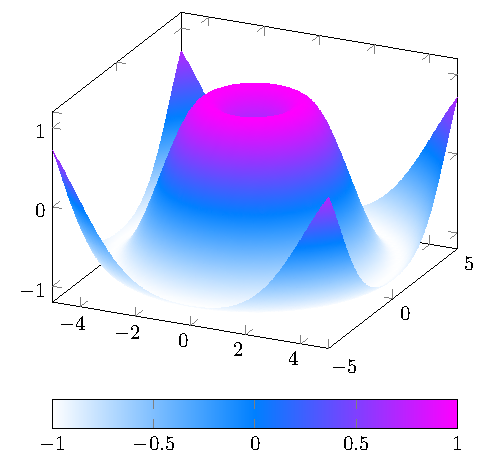
\includegraphics[width=1\linewidth]{7.14.pdf}}
\end{minipage}
&
\begin{minipage}[m]{0.55\textwidth}
\renewcommand\textminus{\mbox{-}}%<<<<<<<<<<<
\begin{lstlisting}[numberstyle=\zebra{red!15}{yellow!15},numbers=left,basicstyle=\scriptsize]
\documentclass [border = .2cm] {standalone}
\usepackage{pgfplots}
\pgfplotsset{compat = newest}

\begin{document}
\begin{tikzpicture}
\begin{axis}[colormap/cool, colorbar horizontal]

\addplot3 [
    domain=-5:5,
    domain y=-5:5,
    samples=50,
    samples y=50,
    surf,
    shader=interp,
] {sin(deg(sqrt(x^2+y^2)))};
\end{axis}
\end{tikzpicture}

\end{document}
\end{lstlisting}
\end{minipage}
\end{tabular}
%#################### 7.12 ####################
\begin{landscape}
\subsection{\hll{Ellipsis in Circuitikz}}
%https://tex.stackexchange.com/questions/232924/ellipsis-in-circuitikz

\begin{tabular}{c | c}
\begin{minipage}[m]{0.65\textwidth}
\enum{
\begin{circuitikz}[line width=1pt]
  \draw (0,2) to[L,l=$L'$,*-*] (2,2)
        (2,0) to[C,l=$C'$,-*] (2,2)
        (2,0) to[short,-*] (0,0)
  ;
  \begin{scope}[xshift=2cm]
  \draw (0,2) to[L,l=$L'$,*-*] (2,2)
        (2,0) to[C,l=$C'$,-*] (2,2)
        (2,0) to[short,-*] (0,0)
  ;
  \end{scope}
  \begin{scope}[xshift=4cm]
  \draw (0,2) to[L,l=$L'$,*-*] (2,2)
        (2,0) to[C,l=$C'$,-*] (2,2)
        (2,0) to[short,-*] (0,0)
  ;
  \end{scope}
  \begin{scope}[xshift=6cm]
  \draw (0,2) --  (2,2)node[midway,scale=2,fill=white]{$\cdots$};
  \draw (0,0) -- (2,0)node[midway,scale=2,fill=white]{$\cdots$};
  \end{scope}
  \draw (8,2) to[L,l=$L'$,-*] (10,2) to[short,-*] (11,2)
        (10,0) to[C,l=$C'$,-*] (10,2)
        (11,0) to[short,*-](10,0) to[short,*-] (8,0)
  ;
\end{circuitikz}}{\thesubsection}
\end{minipage}
&
\begin{minipage}[m]{0.5\textwidth}
\renewcommand\textminus{\mbox{-}}%<<<<<<<<<<<
\begin{lstlisting}[numberstyle=\zebra{red!15}{yellow!15},numbers=left,basicstyle=\scriptsize]
\documentclass{article}
\usepackage{circuitikz}
\ctikzset{bipoles/thickness =1}
\begin{document}
\begin{circuitikz}[line width=1pt]
  \draw (0,2) to[L,l=$L'$,*-*] (2,2)
        (2,0) to[C,l=$C'$,-*] (2,2)
        (2,0) to[short,-*] (0,0)
  ;
  \begin{scope}[xshift=2cm]
  \draw (0,2) to[L,l=$L'$,*-*] (2,2)
        (2,0) to[C,l=$C'$,-*] (2,2)
        (2,0) to[short,-*] (0,0)
  ;
  \end{scope}
  \begin{scope}[xshift=4cm]
  \draw (0,2) to[L,l=$L'$,*-*] (2,2)
        (2,0) to[C,l=$C'$,-*] (2,2)
        (2,0) to[short,-*] (0,0)
  ;
  \end{scope}
  \begin{scope}[xshift=6cm]
  \draw (0,2) --  (2,2)node[midway,scale=2,fill=white]{$\cdots$};
  \draw (0,0) -- (2,0)node[midway,scale=2,fill=white]{$\cdots$};
  \end{scope}
  \draw (8,2) to[L,l=$L'$,-*] (10,2) to[short,-*] (11,2)
        (10,0) to[C,l=$C'$,-*] (10,2)
        (11,0) to[short,*-](10,0) to[short,*-] (8,0)
  ;
\end{circuitikz}
\end{document}
\end{lstlisting}
\end{minipage}
\end{tabular}

\end{landscape}
%#################### 7.13 ####################
\subsection{\hll{A cycle diagram}}

\begin{tabular}{c | c}
\begin{minipage}[m]{0.4\textwidth}
\href{https://texample.net/tikz/examples/pdca-cycle/}{
\begin{tikzpicture}
\fill[even odd rule,mymagenta] circle (1.5);
\node at (0,0) [
font  = \mytextstyle,
color = white,
align = center
]{PDCA\\Cycle};
\arcarrow{ 85}{  3}{ PLAN  }
\arcarrow{270}{357}{ DO    }
\arcarrow{182}{269}{ CHECK }
\arcarrow{176}{ 96}{ ACT   }
\end{tikzpicture}
}
\end{minipage}
&
\begin{minipage}[m]{0.55\textwidth}
\renewcommand\textminus{\mbox{-}}%<<<<<<<<<<<
\begin{lstlisting}[numberstyle=\zebra{red!15}{yellow!15},numbers=left,basicstyle=\scriptsize]
\documentclass[tikz,border=10pt]{standalone}
\usetikzlibrary{decorations.text}
\definecolor{mygray}{RGB}{208,208,208}
\definecolor{mymagenta}{RGB}{226,0,116}
\newcommand*{\mytextstyle}{\sffamily\Large\bfseries\color{black!85}}
\newcommand{\arcarrow}[3]{%
% inner radius, middle radius, outer radius, start angle,
% end angle, tip protusion angle, options, text
\pgfmathsetmacro{\rin}{1.7}
\pgfmathsetmacro{\rmid}{2.2}
\pgfmathsetmacro{\rout}{2.7}
\pgfmathsetmacro{\astart}{#1}
\pgfmathsetmacro{\aend}{#2}
\pgfmathsetmacro{\atip}{5}
\fill[mygray, very thick] (\astart+\atip:\rin)
arc (\astart+\atip:\aend:\rin)
-- (\aend-\atip:\rmid)
-- (\aend:\rout)   arc (\aend:\astart+\atip:\rout)
-- (\astart:\rmid) -- cycle;
\path[
decoration = {
text along path,
text = {|\mytextstyle|#3},
text align = {align = center},
raise = -1.0ex
},
decorate
](\astart+\atip:\rmid) arc (\astart+\atip:\aend+\atip:\rmid);
}
\begin{document}
\begin{tikzpicture}
\fill[even odd rule,mymagenta] circle (1.5);

\node at (0,0) [
font  = \mytextstyle,
color = white,
align = center
]{PDCA\\Cycle};
\arcarrow{ 85}{  3}{ PLAN  }
\arcarrow{270}{357}{ DO    }
\arcarrow{182}{269}{ CHECK }
\arcarrow{176}{ 96}{ ACT   }
\end{tikzpicture}
\end{document}
\end{lstlisting}
\end{minipage}
\end{tabular}

%#################### 7.15 ####################
\subsection{\hll{Rotated polygons}}

\begin{tabular}{c | c}
\begin{minipage}[m]{0.4\textwidth}
\vspace{-1cm}
\enum{\centering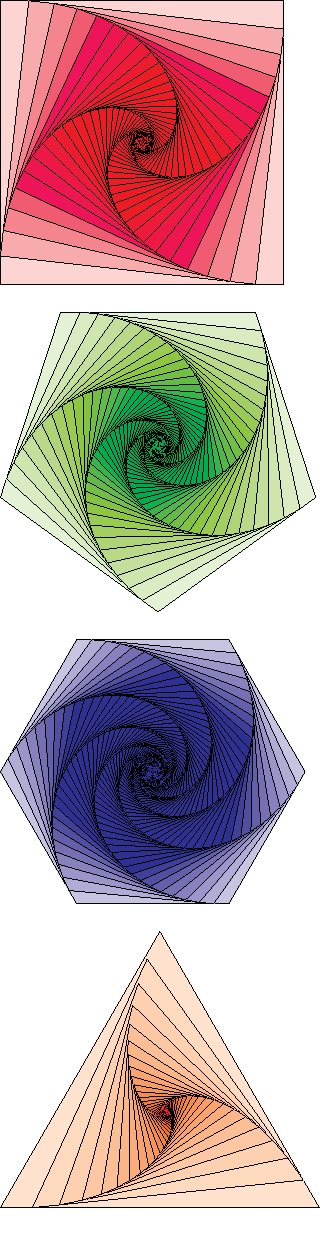
\includegraphics[width=0.88\linewidth]{7.15.pdf}}{\thesubsection}
\end{minipage}
&
\begin{minipage}[m]{0.55\textwidth}
\renewcommand\textminus{\mbox{-}}%<<<<<<<<<<<
\begin{lstlisting}[numberstyle=\zebra{red!15}{yellow!15},numbers=left,basicstyle=\scriptsize]
\documentclass{article}
\usepackage[usenames,dvipsnames,pdftex]{xcolor}
\usepackage{tikz, ifthen}
\newcounter{density}

\newcommand{\square}[2]{
\setcounter{density}{20}
\begin{tikzpicture}[scale=#1]
\def\couleur{#2}
\path[coordinate] (0,0)  coordinate(A)
++( 90:12cm) coordinate(B)
++(0:12cm) coordinate(C)
++(-90:12cm) coordinate(D);
\draw[fill=\couleur!\thedensity] (A) -- (B) -- (C) --(D) -- cycle;
\foreach \x in {1,...,50}{%
\pgfmathsetcounter{density}{\thedensity+20}
\setcounter{density}{\thedensity}
\path[coordinate] coordinate(X) at (A){};
\path[coordinate] (A) -- (B) coordinate[pos=.10](A)-- (C) coordinate[pos=.10](B)-- (D) coordinate[pos=.10](C)-- (X) coordinate[pos=.10](D);
\draw[fill=\couleur!\thedensity] (A)--(B)--(C)-- (D) -- cycle;}
\end{tikzpicture}}

\newcommand{\pentagon}[2]{
\setcounter{density}{20}
\begin{tikzpicture}[scale=#1]
\def\couleur{#2}
\path[coordinate] (0,0)  coordinate(A)
++( 144:10cm) coordinate(B)++(72:10cm) coordinate(C)
++(0:10cm) coordinate(D)++(-72:10cm) coordinate(E);
\draw[fill=\couleur!\thedensity] (A) -- (B) -- (C) --(D) -- (E) --  cycle;
\foreach \x in {1,...,80}{%
\pgfmathsetcounter{density}{\thedensity+10}
\setcounter{density}{\thedensity}
\path[coordinate] coordinate(X) at (A){};
\path[coordinate] (A) -- (B) coordinate[pos=.10](A)-- (C) coordinate[pos=.10](B)-- (D) coordinate[pos=.10](C)-- (E) coordinate[pos=.10](D)-- (X) coordinate[pos=.10](E);
\draw[fill=\couleur!\thedensity] (A)--(B)--(C)-- (D) --(E)  -- cycle;}
\end{tikzpicture}}

\newcommand{\trianglee}[2]{
\begin{tikzpicture}[scale=#1]
\def\couleur{#2}
\path[coordinate] (-1,0) coordinate(A)++(0:6cm) coordinate(B)++(120:6cm) coordinate(C);
\pgfmathsetcounter{density}{20}
\setcounter{density}{\thedensity}
\draw[fill=\couleur!\thedensity] (A) -- (B) -- (C) -- cycle;
\foreach \x in {1,...,40}{%
\pgfmathsetcounter{density}{\thedensity + 7} 
\setcounter{density}{\thedensity}
\path[coordinate] (A) -- (B) coordinate[pos=.1](A)-- (C) coordinate[pos=.1](B)
-- cycle coordinate[pos=.1](C);
\draw[fill=\couleur!\thedensity] (A) -- (B) -- (C) -- cycle;}
\end{tikzpicture}}

\begin{document}
\square{0.3}{OrangeRed}
\pentagon{0.3}{LimeGreen}
\trianglee{0.5}{Violet}
\end{document}
\end{lstlisting}
Source: \href{https://texample.net//tikz/examples/rotated-polygons/}{https://texample.net//tikz/examples/rotated-polygons/}
\end{minipage}
\end{tabular}

%#################### 7.16 ####################
%#################### 7.17 ####################
















%------------------C8
\chapter{Highlighting}
%#################### 8.1 ####################
\subsection{\hll{Words highlighting \xmybox{1}}}
\begin{table}[h!]
\begin{tabular}{c | c}
\begin{minipage}[m]{0.4\textwidth}
\enum{The \mybox[green]{quick} brown \mybox{fox} \mybox[blue]{jumps} over the
\mybox[green]{lazy} \mybox{dog}.\par
The \xmybox[green]{quick} brown \xmybox{fox} \xmybox[blue]{jumps} over the
\xmybox[green]{lazy} \xmybox{dog}.}{8.1}

\end{minipage}
&
\begin{minipage}[m]{0.55\textwidth}
\renewcommand\textminus{\mbox{-}}%<<<<<<<<<<<
\begin{lstlisting}[numberstyle=\zebra{green!15}{yellow!15},numbers=left,basicstyle=\ttfamily\footnotesize]{tex}
\documentclass{article}
\usepackage{tcolorbox}
\newtcbox{\mybox}[1][red]{on line,
arc=0pt,outer arc=0pt,colback=#1!10!white,colframe=#1!50!black,
boxsep=0pt,left=1pt,right=1pt,top=2pt,bottom=2pt,
boxrule=0pt,bottomrule=1pt,toprule=1pt}
\newtcbox{\xmybox}[1][red]{on line,
arc=7pt,colback=#1!10!white,colframe=#1!50!black,
before upper={\rule[-3pt]{0pt}{10pt}},boxrule=1pt,
boxsep=0pt,left=6pt,right=6pt,top=2pt,bottom=2pt}
\begin{document}
The \mybox[green]{quick} brown \mybox{fox}...\par
The \xmybox[green]{quick} brown \xmybox{fox} ...
\end{document}
\end{lstlisting}
\end{minipage}
\end{tabular}
\end{table}
%#################### 8.2 ####################
\subsection{\hll{Unusual words highlighting}}
\begin{table}[h!]
\begin{tabular}{c | c}
\begin{minipage}[m]{0.4\textwidth}
\enum{
Here You can see \mylib{\href{https://texdoc.org/serve/tcolorbox.pdf/0}{more examples}} and learn something new.}{8.2}
\end{minipage}
&
\begin{minipage}[m]{0.55\textwidth}
\renewcommand\textminus{\mbox{-}}%<<<<<<<<<<<
\begin{lstlisting}[numberstyle=\zebra{green!15}{yellow!15},numbers=left,basicstyle=\ttfamily\scriptsize]{tex}
\usepackage[many]{tcolorbox}
\newtcbox{\mylib}{enhanced,nobeforeafter, tcbox raise base, boxrule=0.4pt, top=0mm, bottom=0mm,
  right=0mm, left=4mm, arc=1pt, boxsep=2pt, before upper={\vphantom{dlg}},  colframe=green!50!black, coltext=green!25!black, colback=green!10!white,  overlay={\begin{tcbclipinterior} \fill[green!75!blue!50!white] (frame.south west) rectangle node[text=white,font=\sffamily\bfseries\tiny,rotate=90] {TYP} ([xshift=4mm]frame.north west);\end{tcbclipinterior}}}
\begin{document}
\mylib{recieve}
\end{document}
\end{lstlisting}
\end{minipage}
\end{tabular}
\end{table}
\clearpage

%#################### 8.3 ####################
\subsection{\hll{Colored circles}}
\begin{table}[h!]
\begin{tabular}{c | c}
\begin{minipage}[m]{0.4\textwidth}
\enum{
\circled[fill=amber,draw=black]{1} 
\circled[fill=babyblue,draw=black]{2} 
\circled[fill=green,draw=black]{3}  
$\cdots$\circled[fill=green!75!blue!50!white,draw=black]{4} 
\circled[fill=orange,draw=black]{5} 
\circled[fill=purple!70!white,draw=black]{6}}{8.3}
\end{minipage}
&
\begin{minipage}[m]{0.55\textwidth}
\renewcommand\textminus{\mbox{-}}%<<<<<<<<<<<
\begin{lstlisting}[numberstyle=\zebra{green!15}{yellow!15},numbers=left,basicstyle=\ttfamily\scriptsize]{tex}
\usepackage{tikz}
\usepackage[framemethod=TikZ]{mdframed}
\usepackage{xcolor}
\usetikzlibrary{calc}
\makeatletter
\newlength{\mylength}
\xdef\CircleFactor{1.1}
\setlength\mylength{\dimexpr\f@size pt}
\newsavebox{\mybox}
\newcommand*\circled[2][draw=blue]{\savebox\mybox{\vbox{\vphantom{WL1/}#1}}\setlength\mylength{\dimexpr\CircleFactor\dimexpr\ht\mybox+\dp\mybox\relax\relax}\tikzset{mystyle/.style={circle,#1,minimum height={\mylength}}}	\tikz[baseline=(char.base)]
\node[mystyle] (char) {#2};}
\makeatother
\definecolor{amber}{rgb}{1.0, 0.75, 0.0}
\definecolor{babyblue}{rgb}{0.54, 0.81, 0.94}
usage -->  \circled[fill=amber,draw=black]{1} 
\end{lstlisting}
\end{minipage}
\end{tabular}
\end{table}

%#################### 8.4 ####################
\subsection{\hll{Whole line colored}}
\begin{table}[h!]
\begin{tabular}{c | c}
\begin{minipage}[m]{0.4\textwidth}
\enum{
\hly{green}{some text}
\hly{yellow}{some text}
\hly{red}{some text}}{8.4}
\end{minipage}
&
\begin{minipage}[m]{0.55\textwidth}
\renewcommand\textminus{\mbox{-}}%<<<<<<<<<<<
\begin{lstlisting}[numberstyle=\zebra{green!15}{yellow!15},numbers=left,basicstyle=\ttfamily\scriptsize]{tex}
\documentclass{article}
\usepackage{xcolor}
\newcommand{\hly}[2]{\colorbox{#1!80}{\parbox{\textwidth}{#2}}}

\begin{document}
%\hly{YOURcolor}{some text}
\hly{green}{some text}
\hly{yellow}{some text}
\hly{red}{some text}
\end{document}
\end{lstlisting}
\end{minipage}
\end{tabular}
\end{table}

%#################### 8.5 ####################
\subsection{\hll{Circle text in points to other text}}
\begin{table}[h!]
\begin{tabular}{c | c}
\begin{minipage}[m]{0.4\textwidth}
\enum{\tikzset{mynode/.style={inner sep=2pt,fill=cyan!50,draw=blue,line width=1pt,rounded corners}}

\tikzmarknode[mynode]{A}{This} is just some text that I will repeat for this section again and again. This is just some text that I will repeat for this section again and again. 

\begin{tikzpicture}[remember picture, overlay]
    \draw[->,line width=1pt,blue] (A) --++ (1,1) node[above right] {your comment here};
\end{tikzpicture}}{8.5}
\end{minipage}
&
\begin{minipage}[m]{0.55\textwidth}
\renewcommand\textminus{\mbox{-}}%<<<<<<<<<<<
\begin{lstlisting}[numberstyle=\zebra{green!15}{yellow!15},numbers=left,basicstyle=\ttfamily\scriptsize]{tex}
\documentclass{article}
\usepackage{tikz}
\usetikzlibrary{tikzmark}

\begin{document}
\tikzset{mynode/.style={inner sep=2pt,fill=cyan!50,draw=blue,line width=1pt,rounded corners}}

This is just some \tikzmarknode[mynode]{A}{text that} I will repeat for this section again and again. This is just some text that I will repeat for this section again and again. 

\begin{tikzpicture}[remember picture, overlay]
    \draw[->,line width=1pt,blue] (A) --++ (1,1) node[above right] {your comment here};
\end{tikzpicture}

\end{document}
\end{lstlisting}
\end{minipage}
\end{tabular}
\end{table}
\clearpage

%#################### 8.6 ####################
\subsection{\hll{Keybutton}}
\begin{table}[h!]
\begin{tabular}{c | c}
\begin{minipage}[m]{0.4\textwidth}
\enum{Press \button{alt } + \button{F4 } for help !}{8.6}
\end{minipage}
&
\begin{minipage}[m]{0.55\textwidth}
\renewcommand\textminus{\mbox{-}}%<<<<<<<<<<<
\begin{lstlisting}[numberstyle=\zebra{green!15}{yellow!15},numbers=left,basicstyle=\ttfamily\scriptsize]{tex}
\documentclass[10pt]{article}
\usepackage{tikz}
\usetikzlibrary{shadows}
\tikzstyle{buttonstyle} = [rectangle, fill = black!30, draw = black!80, drop shadow, font={\sffamily\bfseries}, text=white]
\newcommand*{\button}[1]{\tikz{\node[buttonstyle] {#1};}}

\begin{document}
Press \button{F5} for help !
\end{document}
\end{lstlisting}
\end{minipage}
\end{tabular}
\end{table}


%#################### 8.7 ####################
\subsection{\hll{Colorful \xmyboxg{$\backslash$tableofcontents}}}
\begin{table}[h!]
\begin{tabular}{c | c}
\begin{minipage}[m]{0.4\textwidth}
\enum{Press \button{alt } + \button{F4 } for help !}{8.6}
\end{minipage}
&
\begin{minipage}[m]{0.55\textwidth}
\renewcommand\textminus{\mbox{-}}%<<<<<<<<<<<
\begin{lstlisting}[numberstyle=\zebra{green!15}{yellow!15},numbers=left,basicstyle=\ttfamily\scriptsize]{tex}
\documentclass{article}
\usepackage{tocloft}
\usepackage{xcolor}
\usepackage{tikz}
\usetikzlibrary{backgrounds}
\usetikzlibrary{calc}

\newcounter{seccntr}
\setcounter{seccntr}{-1}

\newcommand*{\hnode}[1]{%
\tikz[remember picture] \node[minimum size=0pt,inner sep=0pt,outer sep=4.5pt] (#1) {};}
% create a node at the beginning of the section entry
\renewcommand{\cftsecfont}{\hnode{P1}\bfseries\Large
\stepcounter{seccntr}%
\ifcase\value{seccntr}%
\tikz[remember picture,overlay] \draw (P1.north west)  [line width={17pt}, red,opacity=0.3] -- ++($(\textwidth,0) + (1ex,0)$);
%--- 0 --
\or\tikz[remember picture,overlay] \draw (P1.north west)  [line width={17pt}, green,opacity=0.4] -- ++($(\textwidth,0) + (1ex,0)$);%--- 1 --
\or\tikz[remember picture,overlay]  \draw (P1.north west)  [line width={17pt}, yellow,opacity=1] -- ++($(\textwidth,0) + (1ex,0)$);%--- 2 --
\or\tikz[remember picture,overlay]  \draw (P1.north west)  [line width={17pt}, blue,opacity=0.6] -- ++($(\textwidth,0) + (1ex,0)$);%--- 3 --
\or\tikz[remember picture,overlay]  \draw (P1.north west)  [line width={17pt}, orange,opacity=0.7] -- ++($(\textwidth,0) + (1ex,0)$);%-- default
\else\tikz[remember picture,overlay] \draw (P1.north west)  [line width={17pt}, gray,opacity=0.8] -- ++($(\textwidth,0) + (1ex,0)$);%-- default
\fi  %
}
\renewcommand{\cftsecpagefont}{\bfseries}

\begin{document}
\tableofcontents

\section{First Section}
\subsection{\hll{A subsubsection}}
\subsection{\hll{A subsubsection}}
\section{Second Section}
\subsection{\hll{A subsubsection}}
\section{Third Section}
\end{document}
\end{lstlisting}
\end{minipage}
\end{tabular}
\end{table}

%#################### 8.8 ####################



%------------------C9
\chapter{For Fun}
%#################### 9.1 ####################
\subsection{\hll{LaTeX Coffee Stains}}
\begin{table}[h!]
\begin{tabular}{c | c}
\begin{minipage}[m]{0.4\textwidth}
\enum{\cofeAm{1}{0.6}{0}{0.cm}{6.5cm} 

\cofeCm{0.9}{0.5}{180}{-7.cm}{11cm}

Download \fbox{coffee4.sty} and put in the same directory

\cofeDm{0.2}{0.2}{90}{0.5cm}{2.5cm}
\cofeBm{0.5}{0.5}{0}{-3.cm}{10cm}

 }{\href{https://www.overleaf.com/latex/examples/latex-coffee-stains/qsjjwwsrmwnc}{9.1}}

\end{minipage}
&
\begin{minipage}[m]{0.55\textwidth}
\renewcommand\textminus{\mbox{-}}%<<<<<<<<<<<

\begin{lstlisting}[numberstyle=\zebra{orange!15}{red!15},numbers=left,basicstyle=\ttfamily\footnotesize]
\documentclass{article}
\usepackage{tikz}
\usetikzlibrary{arrows,shapes}
\usepackage{coffee4}
\enum{\cofeAm{1}{0.6}{0}{0.cm}{6cm} 
\cofeCm{0.9}{0.5}{180}{-7.cm}{11cm}
\cofeDm{0.4}{0.2}{90}{1.0cm}{3.0cm}
\cofeBm{0.5}{0.5}{0}{-3.cm}{10cm}
%\cofeAm{alpha}{scale}{angle}{xoff}{yoff} <-- usage
\end{document}
\end{lstlisting}
\end{minipage}
\end{tabular}
\end{table}
%#################### 9.2 ####################
\subsection{\hll{Sticky notes}}
\begin{table}[h!]
\begin{tabular}{c | c}
\begin{minipage}[m]{0.4\textwidth}
\enum{ \href{https://tex.stackexchange.com/questions/26846/how-to-scale-a-tikzpicture-including-texts}{\img{1}{9.3}}}{9.2}

\end{minipage}
&
\begin{minipage}[m]{0.55\textwidth}
\renewcommand\textminus{\mbox{-}}%<<<<<<<<<<<
\begin{lstlisting}[numberstyle=\zebra{orange!15}{red!15},numbers=left,basicstyle=\ttfamily\scriptsize]
\documentclass{article}
\usepackage{xparse}
\usepackage{fancypar}
\usetikzlibrary{calc,shadows}
\NewDocumentCommand\StickyNoteP{O{6cm}mO{6cm}}{%
\begin{tikzpicture}
\node[
drop shadow={shadow xshift=3pt,},
inner xsep=0pt,
xslant=-0.1,yslant=0.1,
inner ysep=0pt,
text depth=\the\dimexpr#1+2.5ex\relax
] {\parbox[t][#1][c]{#3}{#2}};
\end{tikzpicture}}

\begin{document}
\StickyNoteP[2.5cm]{%
\NotebookPar[spiral=false]{
\LARGE first\\  second }}[6.5cm]
\end{document}
\end{lstlisting}
\end{minipage}
\end{tabular}
\end{table}
\clearpage
%#################### 9.3 ####################
\subsection{\hll{\fadingtext[scale=1, font=\bfseries]{path picture shading=rainbow}{Rainbow text}}}
\begin{table}[h!]
\begin{tabular}{c | c}
\begin{minipage}[m]{0.4\textwidth}
\enum{ \fadingtext[scale=2, font=\bfseries]{upper left=red, upper right=green, lower left=blue,lower right=yellow}{\LaTeX} \fadingtext[scale=2, font=\bfseries]{path picture shading=rainbow}{\LaTeX} \\

\noindent\fadingtext[scale=0.7, font=\bfseries]{path picture shading=rainbow}{\parbox[b]{1.5\linewidth}{\strut\lipsum[1]}}

 }{\href{https://tex.stackexchange.com/questions/344260/rainbow-colored-one-letter-with-tikz-and-xcolor}{9.3}}

\end{minipage}
&
\begin{minipage}[m]{0.55\textwidth}
\renewcommand\textminus{\mbox{-}}%<<<<<<<<<<<
\begin{lstlisting}[numberstyle=\zebra{orange!15}{red!15},numbers=left,basicstyle=\ttfamily\scriptsize]
  \documentclass{article} 
  \usepackage{tikz}
  \usetikzlibrary{fadings, shadings}
  \newcounter{fadcnt}\setcounter{fadcnt}{0}
  \newcommand\fadingtext[3][]{%
  \stepcounter{fadcnt}
    \begin{tikzfadingfrompicture}[name=fading letter\thefadcnt]
      \node[text=transparent!0,inner xsep=0pt,outer xsep=0pt,#1] {#3};
    \end{tikzfadingfrompicture}%
    \begin{tikzpicture}[baseline=(textnode.base)]
      \node[inner sep=0pt,outer sep=0pt,#1](textnode){\phantom{#3}}; 
      \shade[path fading=fading letter\thefadcnt,#2,fit fading=false]
      (textnode.south west) rectangle (textnode.north east);% 
    \end{tikzpicture}% 
  }
  \usetikzlibrary{calc}
  \newbox\shbox
  \tikzset{%
    path picture shading/.style={%
    path picture={%
  %
  \pgfpointdiff{\pgfpointanchor{path picture bounding box}{south west}}%
    {\pgfpointanchor{path picture bounding box}{north east}}%
  \pgfgetlastxy\pathwidth\pathheight%
  \pgfinterruptpicture%
     \global\setbox\shbox=\hbox{\pgfuseshading{#1}}%
   \endpgfinterruptpicture%
  \pgftransformshift{\pgfpointanchor{path picture bounding box}{center}}%
  \pgftransformxscale{\pathwidth/(\wd\shbox)}%
  \pgftransformyscale{\pathheight/(\ht\shbox)}% \dp will (should) be 0pt
  \pgftext{\box\shbox}%
  %
      }
    }
  }
  \pgfdeclarehorizontalshading{rainbow}{10bp}{color(0bp)=(violet);
              color(1.6667bp)=(blue);
              color(3.3333bp)=(cyan);
              color(5bp)=(green);
              color(6.6667bp)=(yellow);
              color(8.3333bp)=(orange);
              color(10bp)=(red)}
  \begin{document} 
   \fadingtext[scale=10, font=\bfseries]{upper left=red, upper right=green, lower left=blue,lower right=yellow}{\LaTeX}

  \fadingtext[scale=10, font=\bfseries]{path picture shading=rainbow}{\LaTeX}

  \noindent\fadingtext[scale=0.7, font=\bfseries]{path picture shading=rainbow}{\parbox[b]{1.5\linewidth}{\strut\lipsum[1]}}
  \end{document}
\end{lstlisting}
\end{minipage}
\end{tabular}
\end{table}
\clearpage

%#################### 9.4 ####################
\subsection{\hll{Single Watermark}}
\begin{table}[h!]
\begin{tabular}{c | c}
\begin{minipage}[m]{0.4\textwidth}
\enum{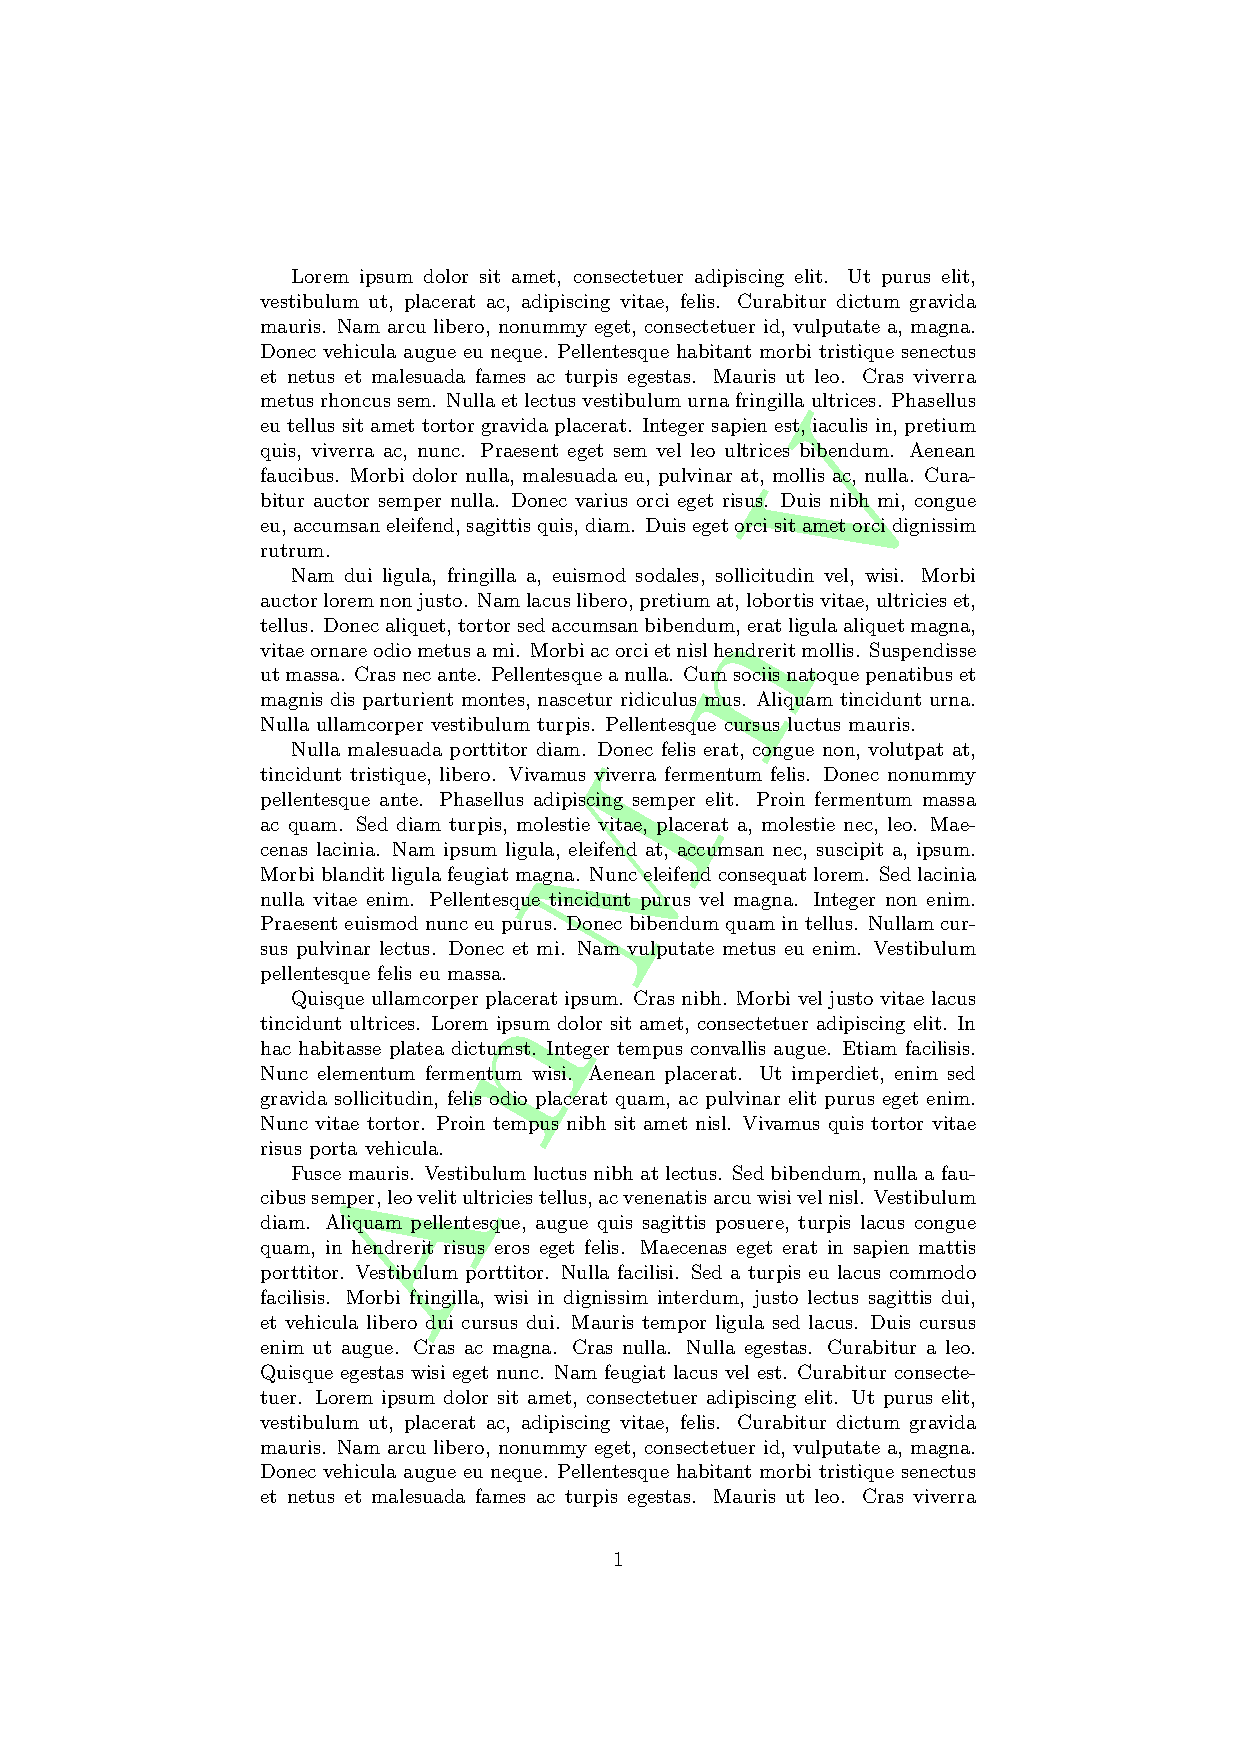
\includegraphics[width=0.9\linewidth]{C:/Users/user/Desktop/eBook/images/9.4/9.4.pdf}}{9.4}

\end{minipage}
&
\begin{minipage}[m]{0.55\textwidth}
\renewcommand\textminus{\mbox{-}}%<<<<<<<<<<<
\begin{lstlisting}[numberstyle=\zebra{orange!15}{red!15},numbers=left,basicstyle=\ttfamily\scriptsize]
\documentclass[a4paper]{article}
\usepackage[T1]{fontenc}
\usepackage[utf8]{inputenc}
\usepackage[pages=some]{background}% change "some" to "all" to see WM on all pages 
\usepackage{lipsum}
\backgroundsetup{color=green, opacity=0.3, scale=10, contents={A n M n V}}

\begin{document}
\lipsum[1-5] 
\BgThispage
\lipsum[1-5]
\end{document}
\end{lstlisting}
\end{minipage}
\end{tabular}
\end{table}
%#################### 9.5 #################### 
\subsection{\hll{Full page of Watermarks}}
\begin{table}[h!]
\begin{tabular}{c | c}
\begin{minipage}[m]{0.4\textwidth}
\enum{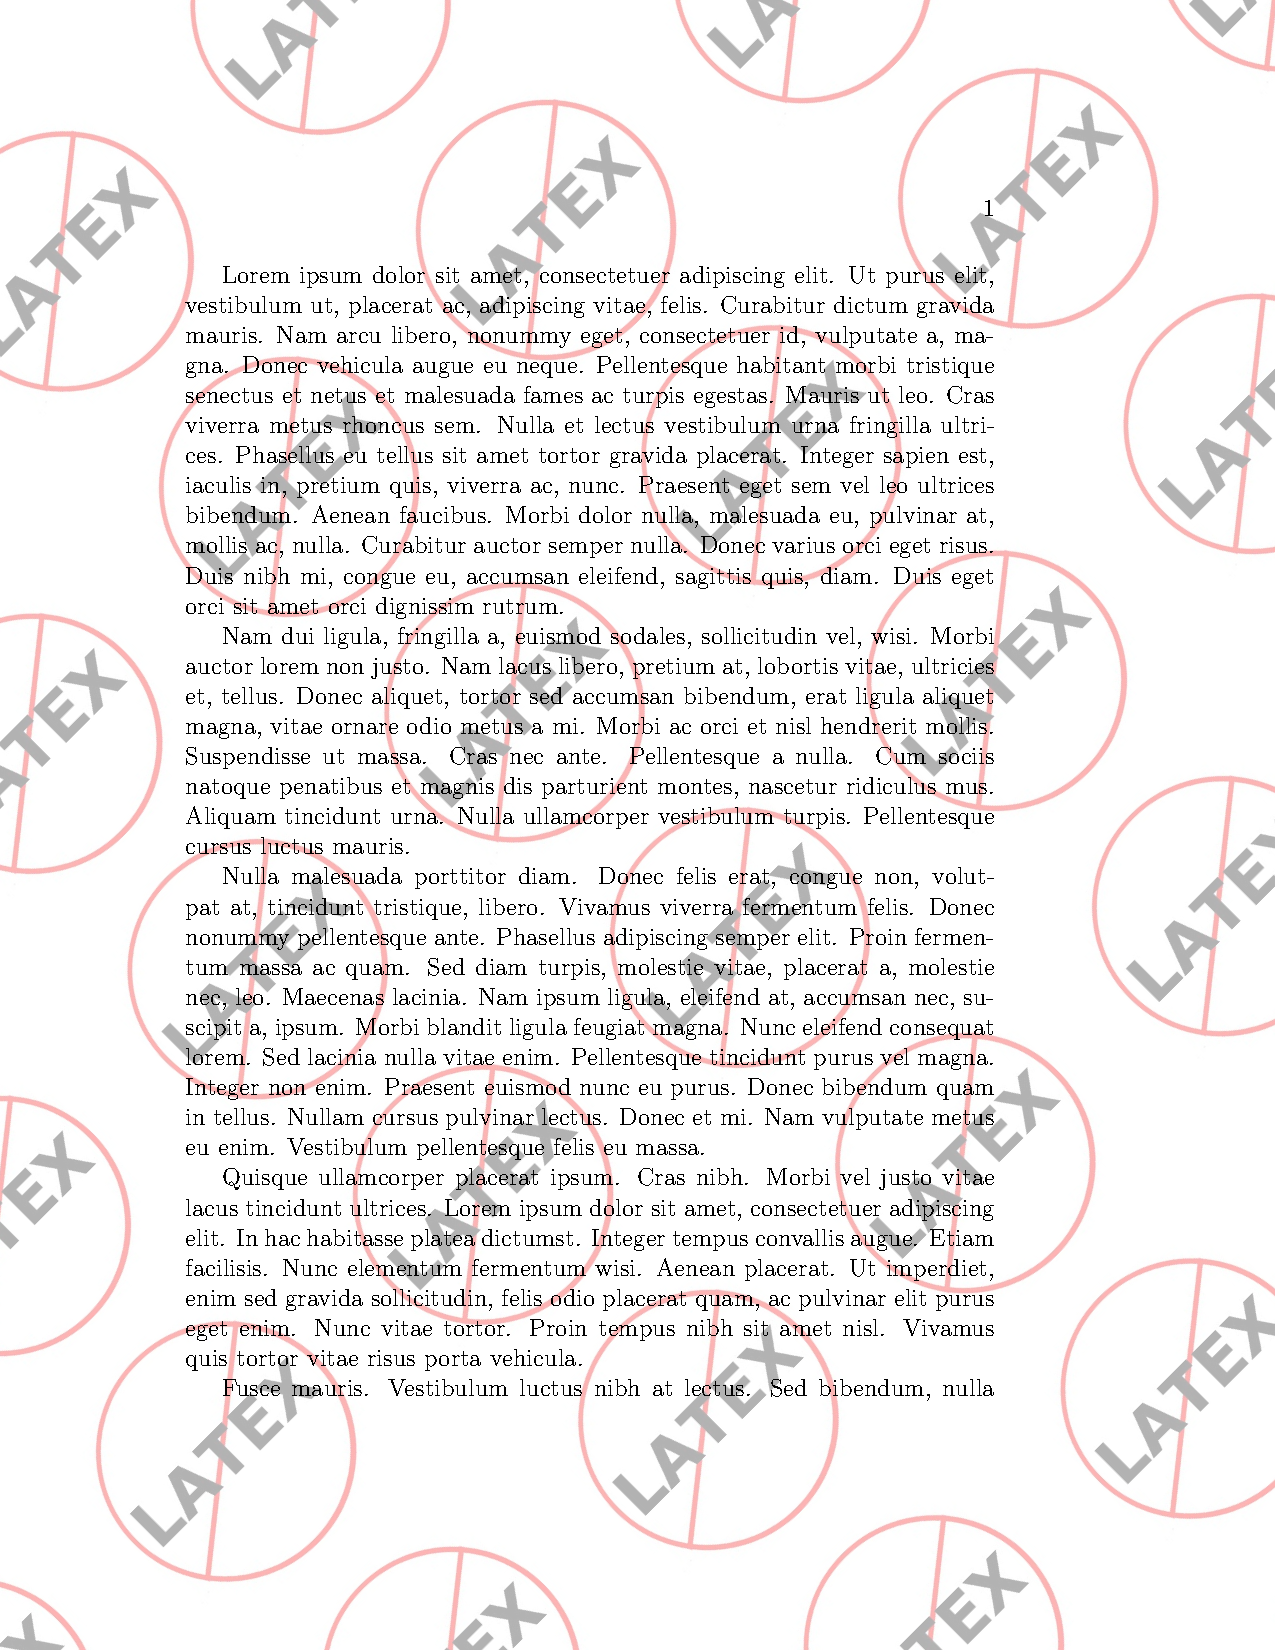
\includegraphics[width=0.9\linewidth]{C:/Users/user/Desktop/eBook/images/9.5/9.5.pdf}}{9.5}

\end{minipage}
&
\begin{minipage}[m]{0.55\textwidth}
\renewcommand\textminus{\mbox{-}}%<<<<<<<<<<<
\begin{lstlisting}[numberstyle=\zebra{orange!15}{red!15},numbers=left,basicstyle=\ttfamily\scriptsize]
\documentclass[12pt]{book}
\usepackage{graphicx}
\usepackage[pages=some]{background}
\usepackage{lipsum}
\newcommand\DupImage{%
     
\includegraphics[width=5cm]{logo.jpeg}\hfill%  YOUR IMAGE
     
\includegraphics[width=5cm]{logo.jpeg}\hfill%  YOUR IMAGE
     
\includegraphics[width=5cm]{logo.jpeg}\hfill%  YOUR IMAGE
     
\includegraphics[width=5cm]{logo.jpeg}\hfill%  YOUR IMAGE
     
\includegraphics[width=5cm]{logo.jpeg}\hfill%  YOUR IMAGE
     
\includegraphics[width=5cm]{logo.jpeg}\hfill%  YOUR IMAGE
     
\includegraphics[width=5cm]{logo.jpeg}\hfill}
\newlength{\drop}
\backgroundsetup{  scale=1, angle=45, opacity=.3, 
  contents={%
     \begin{minipage}{1.5\paperheight}
     \DupImage\\[2ex]
     \DupImage\\[2ex]
     \DupImage\\[2ex]
     \DupImage\\[2ex]
     \DupImage\\[2ex]
     \DupImage\\[2ex]
     \DupImage\\[2ex]
     \DupImage\\[2ex]
     \DupImage\\[2ex]
     \DupImage  \end{minipage}   }  }

\begin{document}
\drop=0.1\textheight \BgThispage \lipsum[1-8]
\end{document}
\end{lstlisting}
\end{minipage}
\end{tabular}
\end{table}

%#################### 9.6 ####################
\subsection{\hll{Generating QR code}}
\begin{table}[h!]
\begin{tabular}{c | c}
\begin{minipage}[m]{0.4\textwidth}
\enum{
\includegraphics[width=0.9\linewidth]{C:/Users/user/Desktop/eBook/images/9.6/9.6.pdf}}{9.6}
\end{minipage}
&
\begin{minipage}[m]{0.55\textwidth}
\renewcommand\textminus{\mbox{-}}%<<<<<<<<<<<
\begin{lstlisting}[numberstyle=\zebra{orange!15}{red!15},numbers=left,basicstyle=\ttfamily\scriptsize]
\documentclass{article} 
\usepackage{qrcode} 

\begin{document}
\qrcode[height=0.5in]{https://github.com/AnMnv/eBook}
\textcolor{blue}{\qrcode[height=0.5in]{https://github.com/AnMnv/eBook}}
\textcolor{green}{\qrcode[height=0.5in]{https://github.com/AnMnv/eBook}} 
\end{document}
\end{lstlisting}
\end{minipage}
\end{tabular}
\end{table}





\newpage
%#################### 9.7 ####################https://tex.stackexchange.com/questions/560627/how-do-make-gradient-colored-qr-code-in-latex#655712
\subsection{\hll{Gradient QR code}}
\begin{table}[h!]
\begin{tabular}{c | c}
\begin{minipage}[m]{0.4\textwidth}
\enum{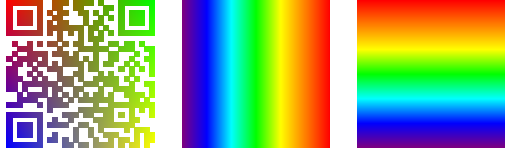
\includegraphics[width=0.9\linewidth]{C:/Users/user/Desktop/eBook/images/9.7/9.7.pdf}}{9.7}
\end{minipage}
&
\begin{minipage}[m]{0.55\textwidth}
\renewcommand\textminus{\mbox{-}}%<<<<<<<<<<<
\begin{lstlisting}[numberstyle=\zebra{orange!15}{red!15},numbers=left,basicstyle=\ttfamily\scriptsize]
\documentclass{article} 
\usepackage{qrcode}[]
\usepackage{tikz}
\usetikzlibrary{fadings, shadings}
\newcounter{fadcnt}\setcounter{fadcnt}{0}
\newcommand\fadingtext[3][]{%
\stepcounter{fadcnt}
  \begin{tikzfadingfrompicture}[name=fading letter\thefadcnt]
    \node[text=transparent!0,inner xsep=0pt,outer xsep=0pt,#1] {#3};
  \end{tikzfadingfrompicture}%
  \begin{tikzpicture}[baseline=(textnode.base)]
    \node[inner sep=0pt,outer sep=0pt,#1](textnode){\phantom{#3}}; 
    \shade[path fading=fading letter\thefadcnt,#2,fit fading=false]
    (textnode.south west) rectangle (textnode.north east);% 
  \end{tikzpicture}}
\usetikzlibrary{calc}
\newbox\shbox
\tikzset{%
  path picture shading/.style={%
  path picture={%
\pgfpointdiff{\pgfpointanchor{path picture bounding box}{south west}}%
  {\pgfpointanchor{path picture bounding box}{north east}}%
\pgfgetlastxy\pathwidth\pathheight%
\pgfinterruptpicture%
   \global\setbox\shbox=\hbox{\pgfuseshading{#1}}%
 \endpgfinterruptpicture%
\pgftransformshift{\pgfpointanchor{path picture bounding box}{center}}%
\pgftransformxscale{\pathwidth/(\wd\shbox)}%
\pgftransformyscale{\pathheight/(\ht\shbox)}% \dp will (should) be 0pt
\pgftext{\box\shbox}%
    }  }  }
\pgfdeclarehorizontalshading{rainbow}{10bp}{color(0bp)=(violet);
            color(1.6667bp)=(blue);
            color(3.3333bp)=(cyan);
            color(5bp)=(green);
            color(6.6667bp)=(yellow);
            color(8.3333bp)=(orange);
            color(10bp)=(red)}
\pgfdeclareverticalshading{rainbow_vertical}{10bp}{color(0bp)=(violet);
            color(1.6667bp)=(blue);
            color(3.3333bp)=(cyan);
            color(5bp)=(green);
            color(6.6667bp)=(yellow);
            color(8.3333bp)=(orange);
            color(10bp)=(red)}

\begin{document}
\fadingtext[scale=0.5]{upper left=red, upper right=green, lower left=blue,lower right=yellow}{\qrcode[height=5cm]{https://github.com/AnMnv/eBook}}
\fadingtext[scale=0.5]{path picture shading=rainbow}{\qrcode[height=5cm]{https://github.com/AnMnv/eBook}}
\fadingtext[scale=0.5]{path picture shading=rainbow_vertical}{\qrcode[height=5cm]{https://github.com/AnMnv/eBook}}
\end{document}
\end{lstlisting}
\end{minipage}
\end{tabular}
\end{table}

%#################### 9.8 ####################LobLib documentation on \href{https://github.com/AnMnv/eBook}{GitHub} in \mybox[black]{LobLib-package} folder.\\ Origins of the package \href{https://github.com/bryce-evans/LobLib}{https://github.com/bryce-evans/LobLib}\\ However, to print lobsters put \mybox[red]{objects} folder and \mybox[red]{loblib.sty} from  the \mybox[black]{LobLib-package} folder into the same directory with your \mybox[brown]{.tex} file.
\subsection{\hll{Lobsrets}}
\begin{table}[h!]
\begin{tabular}{c | c}
\begin{minipage}[m]{0.4\textwidth}
\enum{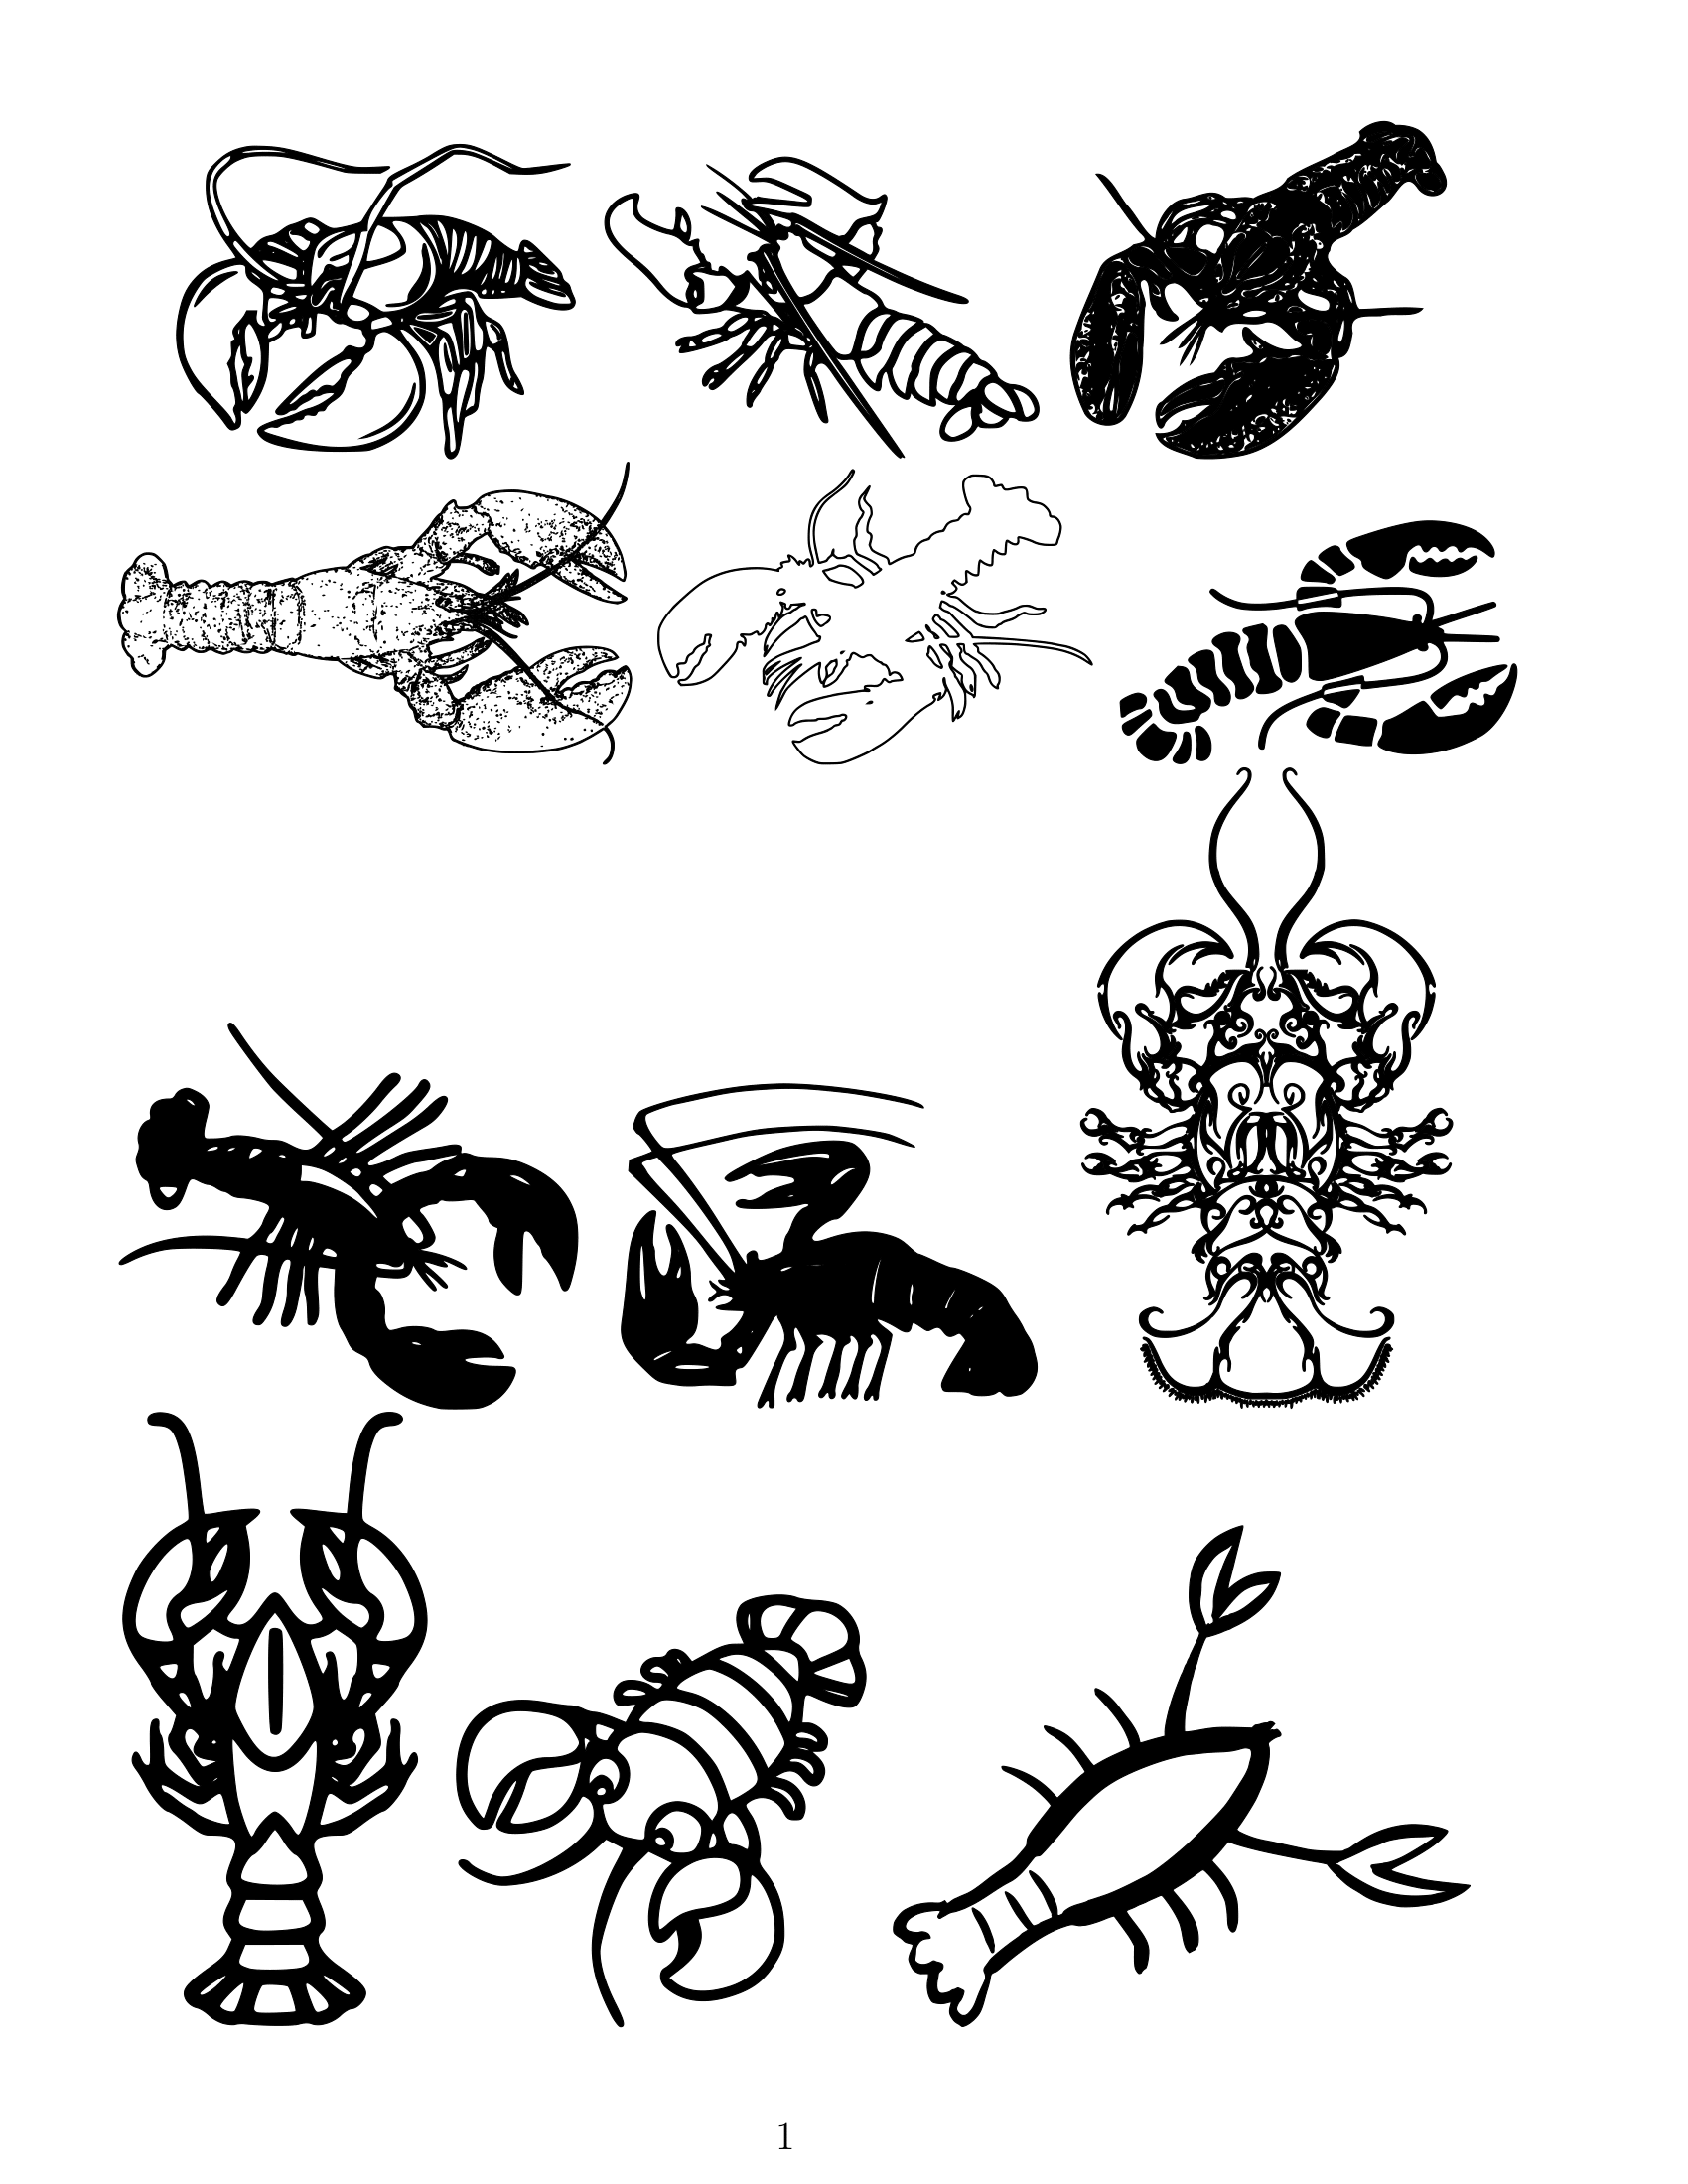
\includegraphics[width=1.2\linewidth]{lobsters_example-1.png}
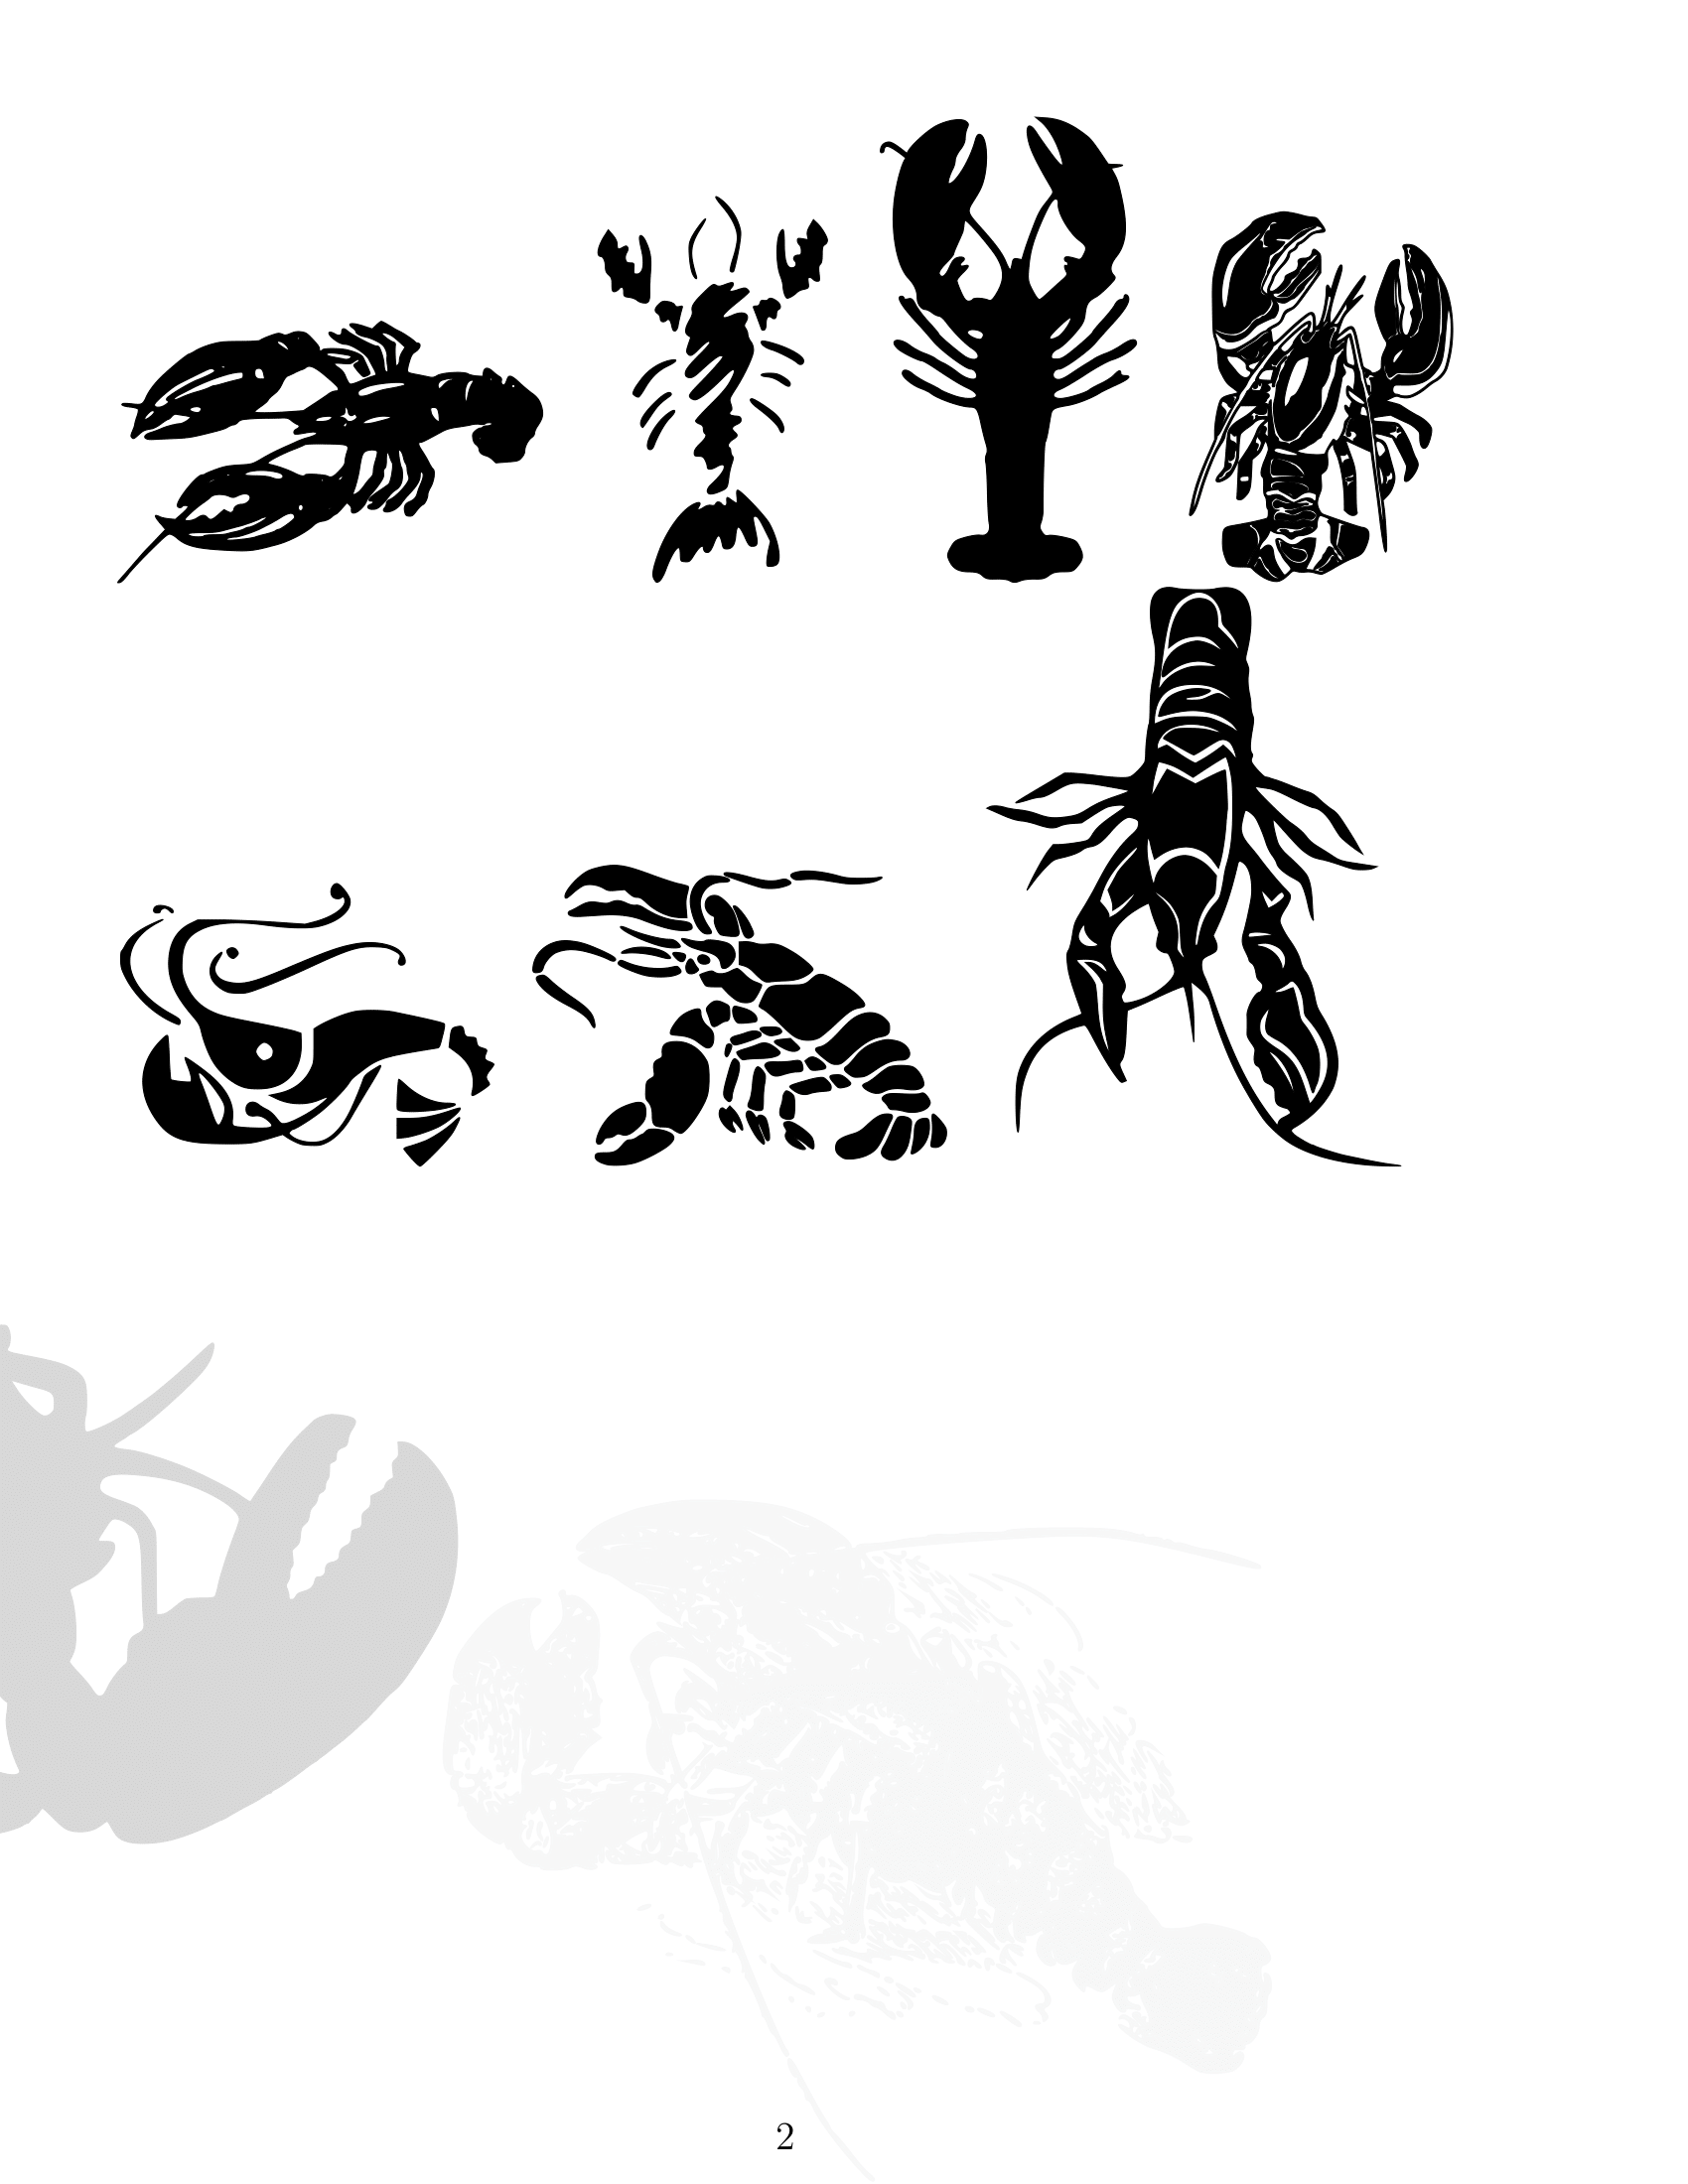
\includegraphics[width=1.2\linewidth]{lobsters_example-2.png}}{9.8}
\end{minipage}
&
\begin{minipage}[m]{0.55\textwidth}
\renewcommand\textminus{\mbox{-}}%<<<<<<<<<<<
\begin{lstlisting}[numberstyle=\zebra{orange!15}{red!15},numbers=left,basicstyle=\ttfamily\scriptsize]
\documentclass[14pt]{extreport}
\usepackage[left=1.5cm,right=3cm,top=1.5cm,
bottom=1.5cm,bindingoffset=0cm]{geometry}
\usepackage{loblib}
 
\begin{document}
\lob{1}     \lob{12}
\lob{2}     \lob{20}
\lob{3}     \lob{21}
\lob{4}     \lob{22}
\lob{5}     \lob{28}
\lob{6}     \lob{32}
\lob{7}     \lob{33}
\lob{8}     \lob{74}
\lob{9}     \lob{76}

\vspace*{2cm}
\hspace*{-2.8cm}
\definecolor{shadow}{rgb}{0.85,0.85,0.85}
\lob[rotate=-90,shadow,xscale=-1.2,yscale=1.2]{77}

\lobwatermark
\end{document}
\end{lstlisting}
LobLib documentation on \href{https://github.com/AnMnv/eBook}{GitHub} in \mybox[black]{LobLib-package} folder.\\ Origins of the package \href{https://github.com/bryce-evans/LobLib}{https://github.com/bryce-evans/LobLib}\\ However, to print lobsters put \mybox[red]{objects} folder and \mybox[red]{loblib.sty} from  the \mybox[black]{LobLib-package} folder into the same directory with your \mybox[brown]{.tex} file.
\end{minipage}
\end{tabular}
\end{table}
%#################### 9.9 ####################
\subsection{\hll{Watermark over \textbf{everything}}}
\begin{table}[h!]
\begin{tabular}{c | c}
\begin{minipage}[m]{0.4\textwidth}
\enum{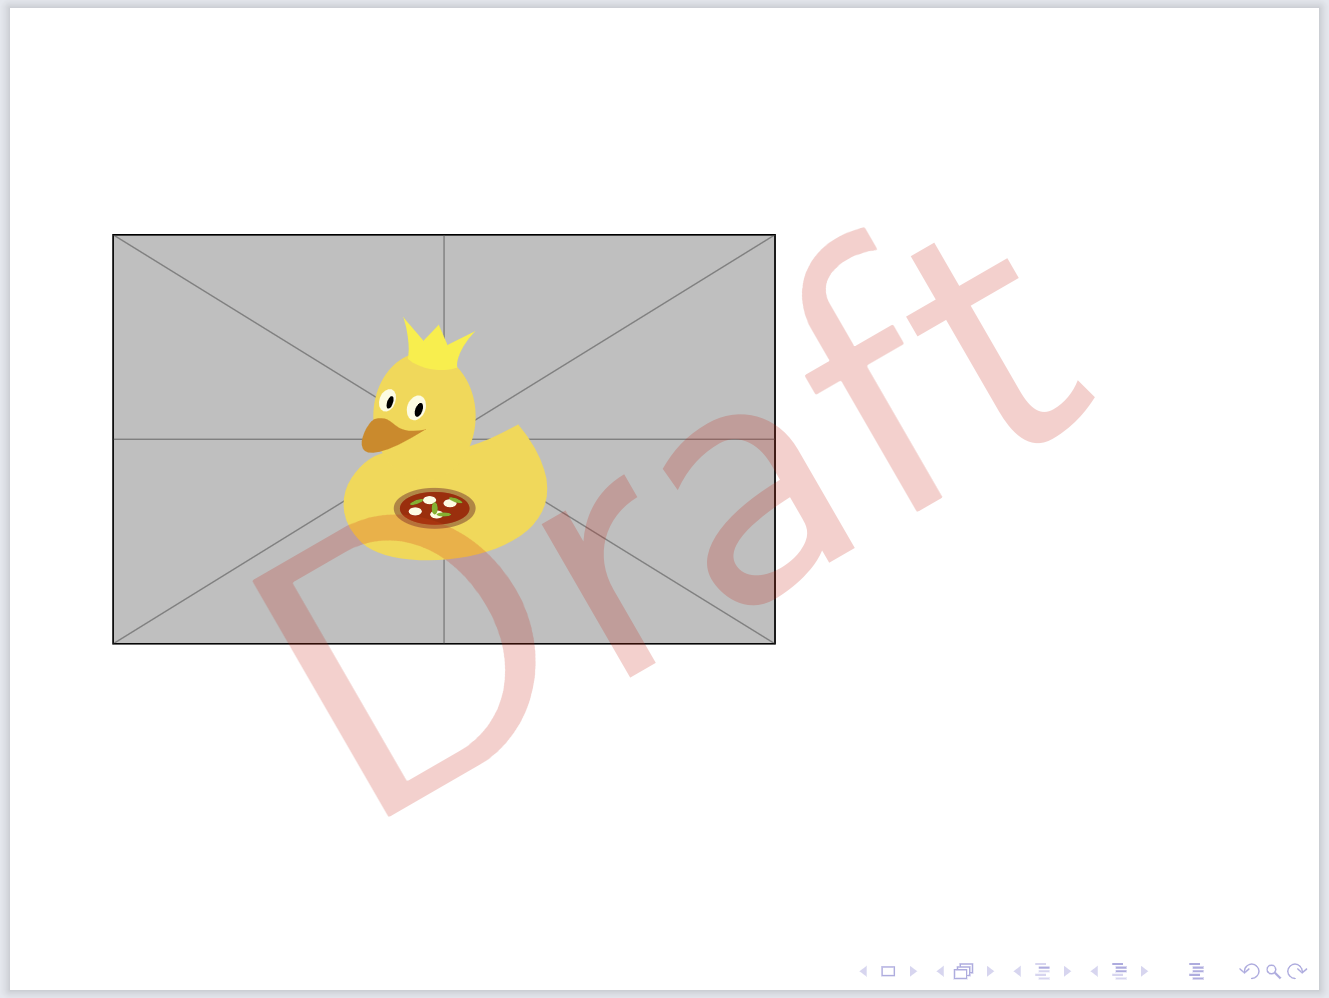
\includegraphics[width=1.\linewidth]{9.9.png}}{9.9}
\end{minipage}
&
\begin{minipage}[m]{0.55\textwidth}
\renewcommand\textminus{\mbox{-}}%<<<<<<<<<<<
\begin{lstlisting}[numberstyle=\zebra{orange!15}{red!15},numbers=left,basicstyle=\ttfamily\scriptsize]
\documentclass{beamer}

\usepackage{tikz}
\AddToHook{shipout/foreground}{
  \begin{tikzpicture}[remember picture,overlay]
    \node[red,rotate=30,scale=10,opacity=0.2] at (current page.center) {Draft}; 
  \end{tikzpicture}}

\begin{document}
\begin{frame}
\includegraphics{example-image-duck}
\end{frame}
\end{document}
\end{lstlisting}
\end{minipage}
\end{tabular}
\end{table}
%#################### 9.10 ####################
\subsection{\hll{Simple Emoji by \href{https://github.com/dilippuri/latexemoji}{dilippuri}}}
\begin{table}[h!]
\begin{tabular}{c | c}
\begin{minipage}[m]{0.4\textwidth}
\enum{\href{https://github.com/dilippuri/latexemoji}{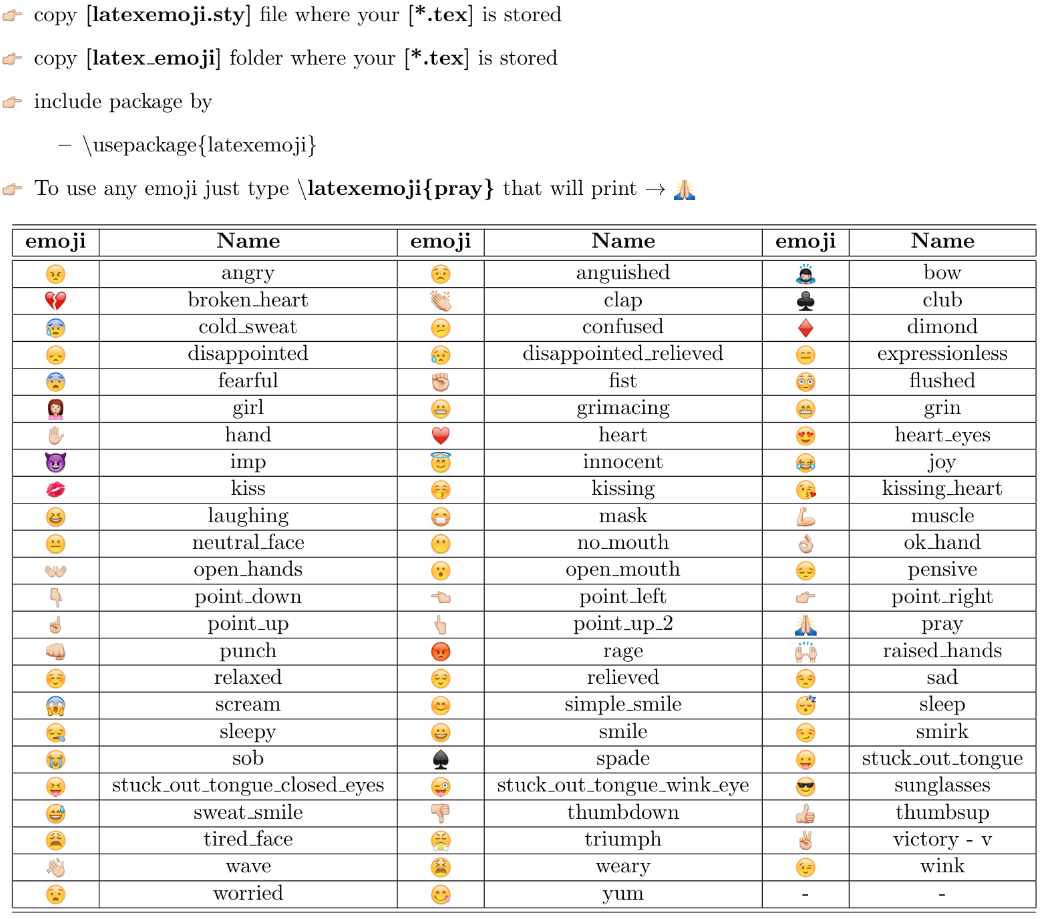
\includegraphics[width=1.\linewidth]{9.10.png}}}{9.10}
\end{minipage}
&
\begin{minipage}[m]{0.55\textwidth}
\renewcommand\textminus{\mbox{-}}%<<<<<<<<<<<
\begin{lstlisting}[numberstyle=\zebra{orange!15}{red!15},numbers=left,basicstyle=\ttfamily\scriptsize]
\documentclass{article} 
\title{This is an example tex file to include emoji in latex}
\author{Dilip Puri}

\begin{document}
\maketitle
Hi, I am (dilippuri) going to include emoji in latex. So I \latexemoji{heart} \LaTeX.\\
I just \latexemoji{stuck_out_tongue_wink_eye}.\\

Good bye! \latexemoji{wave}
\end{document}
\end{lstlisting}
\end{minipage}
\end{tabular}
\end{table}
%#################### 9.11####################
\clearpage
...
\vspace{4cm}
...
\subsection{\hll{Confidential mark/ribbon top right of frontpage}}
\begin{tikzpicture}[
  overlay, 
  remember picture,
  legend/.style={|<->|, gray, font = {\ttfamily}},
  confidential/.style={anchor=center, rotate = -45, font={\sffamily\scshape}}
]
  \coordinate (A) at ($ (current page.north east) + (-\stripskip,0) $);
  \coordinate (A') at ($(A) + (-\stripwidth,0) $);

  \coordinate (B) at ($ (current page.north east) + (0,-\stripskip) $);
  \coordinate (B') at ($(B) + (0,-\stripwidth) $);

  \fill [red] (A) -- (A') -- (B') -- (B) -- cycle;

  \coordinate (tempA) at ($(A)!.5!(A')$);
  \coordinate (tempB) at ($(B)!.5!(B')$);

  \node [confidential](text) at ($(tempA)!.5!(tempB)$) {\Huge Confidential};
\end{tikzpicture}
\begin{table}[h!]
\begin{tabular}{c | c}
\begin{minipage}[m]{0.4\textwidth}
 Look at the top right of the page
\end{minipage}
&
\begin{minipage}[m]{0.55\textwidth}
\renewcommand\textminus{\mbox{-}}%<<<<<<<<<<<
\begin{lstlisting}[numberstyle=\zebra{orange!15}{red!15},numbers=left,basicstyle=\ttfamily\scriptsize]
\documentclass{article} 
\documentclass{scrbook}
\usepackage{lmodern}
\usepackage{tikz}
\usetikzlibrary{calc}
\newcommand{\stripskip}{5}
\newcommand{\stripwidth}{3}

\begin{document}
    \begin{tikzpicture}[
        overlay, 
        remember picture,
        legend/.style={|<->|, gray, font = {\ttfamily}},
        confidential/.style={anchor=center, rotate = -45, font={\sffamily\scshape}}
    ]
        \coordinate (A) at ($ (current page.north east) + (-\stripskip,0) $);
        \coordinate (A') at ($(A) + (-\stripwidth,0) $);

        \coordinate (B) at ($ (current page.north east) + (0,-\stripskip) $);
        \coordinate (B') at ($(B) + (0,-\stripwidth) $);

        \fill [red] (A) -- (A') -- (B') -- (B) -- cycle;

        \coordinate (tempA) at ($(A)!.5!(A')$);
        \coordinate (tempB) at ($(B)!.5!(B')$);

        \node [confidential](text) at ($(tempA)!.5!(tempB)$) {\Huge Confidential};
    \end{tikzpicture}
    \centering \Huge qqqqqqqqq
\end{document}
\end{lstlisting}
\end{minipage}
\end{tabular}
\end{table}
%#################### 9.12 ####################
%#################### 9.13 ####################


%werwer
%------------------C9
\chapter{Animation, videos, interaction}
%#################### 10.1 ####################
\subsection{Video in PDF (okular as a .pdf viewer was used)}
\begin{table}[h!]
\begin{tabular}{c | c}
\begin{minipage}[m]{0.4\textwidth}
\enum{\begin{center}\embedvideo{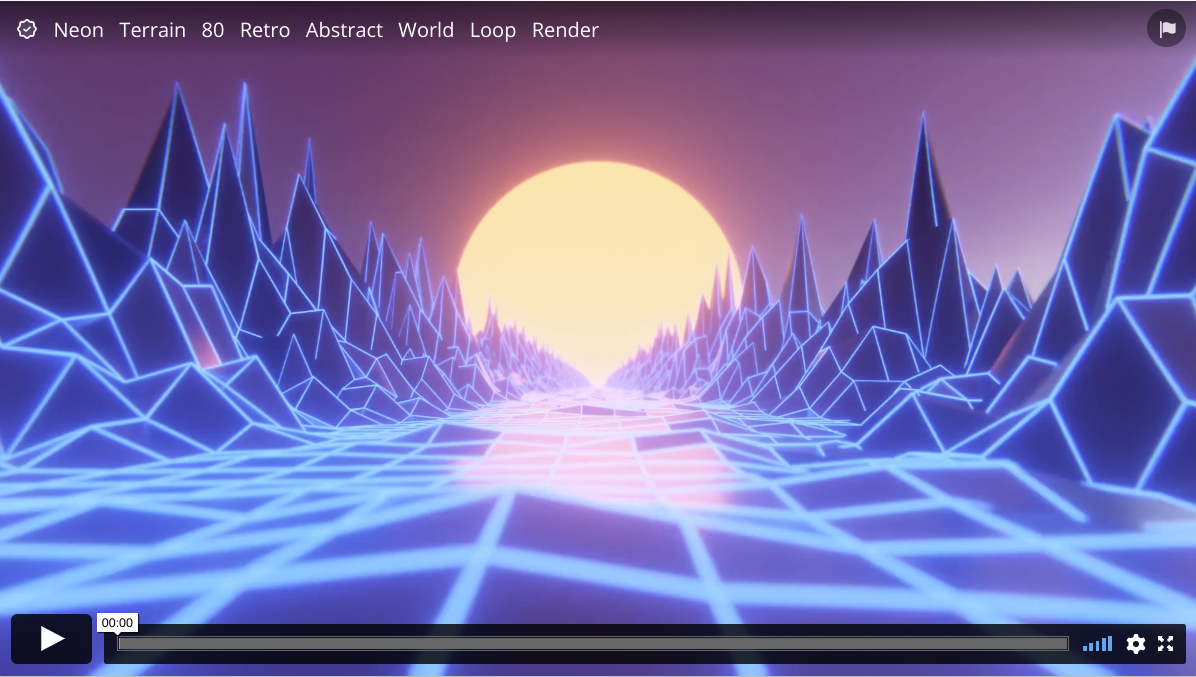
\includegraphics[width=\textwidth]{10.1.png}}{images/10.1.mp4}\end{center}}{10.1}

\end{minipage}
&
\begin{minipage}[m]{0.55\textwidth}
\renewcommand\textminus{\mbox{-}}%<<<<<<<<<<<

\begin{lstlisting}[numberstyle=\zebra{orange!15}{red!15},numbers=left,basicstyle=\ttfamily\tiny]
\documentclass{article}
%%%%%%%%%%%%%%%%%%%%%%%%%%%%%%%%%%%%%%%%%%%%%%%%%%%%%%%%%%%%%%%%%%%%%%%%%%%%%%%
% \embedvideo{<poster or text>}{<video file (MP4+H264)>}
% \embedvideo*{...}{...}                     % auto-play
%%%%%%%%%%%%%%%%%%%%%%%%%%%%%%%%%%%%%%%%%%%%%%%%%%%%%%%%%%%%%%%%%%%%%%%%%%%%%%

\usepackage[bigfiles]{pdfbase}
\ExplSyntaxOn
\NewDocumentCommand\embedvideo{smm}{
  \group_begin:
  \leavevmode
  \tl_if_exist:cTF{file_\file_mdfive_hash:n{#3}}{
    \tl_set_eq:Nc\video{file_\file_mdfive_hash:n{#3}}
  }{
    \IfFileExists{#3}{}{\GenericError{}{File~`#3'~not~found}{}{}}
    \pbs_pdfobj:nnn{}{fstream}{{}{#3}}
    \pbs_pdfobj:nnn{}{dict}{
      /Type/Filespec/F~(#3)/UF~(#3)
      /EF~<</F~\pbs_pdflastobj:>>
    }
    \tl_set:Nx\video{\pbs_pdflastobj:}
    \tl_gset_eq:cN{file_\file_mdfive_hash:n{#3}}\video
  }
  %
  \pbs_pdfobj:nnn{}{dict}{
    /Type/RichMediaInstance/Subtype/Video
    /Asset~\video
    /Params~<</FlashVars (
      source=#3&
      skin=SkinOverAllNoFullNoCaption.swf&
      skinAutoHide=true&
      skinBackgroundColor=0x5F5F5F&
      skinBackgroundAlpha=0
    )>>
  }
  %
  \pbs_pdfobj:nnn{}{dict}{
    /Type/RichMediaConfiguration/Subtype/Video
    /Instances~[\pbs_pdflastobj:]
  }
  %
  \pbs_pdfobj:nnn{}{dict}{
    /Type/RichMediaContent
    /Assets~<<
      /Names~[(#3)~\video]
    >>
    /Configurations~[\pbs_pdflastobj:]
  }
  \tl_set:Nx\rmcontent{\pbs_pdflastobj:}
  %
  \pbs_pdfobj:nnn{}{dict}{
    /Activation~<<
      /Condition/\IfBooleanTF{#1}{PV}{XA}
      /Presentation~<</Style/Embedded>>
    >>
    /Deactivation~<</Condition/PI>>
  }
  %
  \hbox_set:Nn\l_tmpa_box{#2}
  \tl_set:Nx\l_box_wd_tl{\dim_use:N\box_wd:N\l_tmpa_box}
  \tl_set:Nx\l_box_ht_tl{\dim_use:N\box_ht:N\l_tmpa_box}
  \tl_set:Nx\l_box_dp_tl{\dim_use:N\box_dp:N\l_tmpa_box}
  \pbs_pdfxform:nnnnn{1}{1}{}{}{\l_tmpa_box}
  %
  \pbs_pdfannot:nnnn{\l_box_wd_tl}{\l_box_ht_tl}{\l_box_dp_tl}{
    /Subtype/RichMedia
    /BS~<</W~0/S/S>>
    /Contents~(embedded~video~file:#3)
    /NM~(rma:#3)
    /AP~<</N~\pbs_pdflastxform:>>
    /RichMediaSettings~\pbs_pdflastobj:
    /RichMediaContent~\rmcontent
  }
  \phantom{#2}
  \group_end:
}
\ExplSyntaxOff
%%%%%%%%%%%%%%%%%%%%%%%%%%%%%%%%%%%%%%%%%%%%%%%%%%%%%%%%%%%%%%%%%%%%%%%%%%%%%%
\usepackage{graphicx}
\usepackage[hidelinks]{hyperref}


%%%%%%%%This is embed_video.tex (below till \begin{document})%%%%%%%%%%%%% 
\ExplSyntaxOn
\NewDocumentCommand\embedvideo{smm}{
  \group_begin:
  \leavevmode
  \tl_if_exist:cTF{file_\file_mdfive_hash:n{#3}}{
    \tl_set_eq:Nc\video{file_\file_mdfive_hash:n{#3}}
  }{
    \IfFileExists{#3}{}{\GenericError{}{File~`#3'~not~found}{}{}}
    \pbs_pdfobj:nnn{}{fstream}{{}{#3}}
    \pbs_pdfobj:nnn{}{dict}{
      /Type/Filespec/F~(#3)/UF~(#3)
      /EF~<</F~\pbs_pdflastobj:>>
    }
    \tl_set:Nx\video{\pbs_pdflastobj:}
    \tl_gset_eq:cN{file_\file_mdfive_hash:n{#3}}\video
  }
  %
  \pbs_pdfobj:nnn{}{dict}{
    /Type/RichMediaInstance/Subtype/Video
    /Asset~\video
    /Params~<</FlashVars (
      source=#3&
      skin=SkinOverAllNoFullNoCaption.swf&
      skinAutoHide=true&
      skinBackgroundColor=0x5F5F5F&
      skinBackgroundAlpha=0
    )>>
  }
  %
  \pbs_pdfobj:nnn{}{dict}{
    /Type/RichMediaConfiguration/Subtype/Video
    /Instances~[\pbs_pdflastobj:]
  }
  %
  \pbs_pdfobj:nnn{}{dict}{
    /Type/RichMediaContent
    /Assets~<<
      /Names~[(#3)~\video]
    >>
    /Configurations~[\pbs_pdflastobj:]
  }
  \tl_set:Nx\rmcontent{\pbs_pdflastobj:}
  %
  \pbs_pdfobj:nnn{}{dict}{
    /Activation~<<
      /Condition/\IfBooleanTF{#1}{PV}{XA}
      /Presentation~<</Style/Embedded>>
    >>
    /Deactivation~<</Condition/PI>>
  }
  %
  \hbox_set:Nn\l_tmpa_box{#2}
  \tl_set:Nx\l_box_wd_tl{\dim_use:N\box_wd:N\l_tmpa_box}
  \tl_set:Nx\l_box_ht_tl{\dim_use:N\box_ht:N\l_tmpa_box}
  \tl_set:Nx\l_box_dp_tl{\dim_use:N\box_dp:N\l_tmpa_box}
  \pbs_pdfxform:nnnnn{1}{1}{}{}{\l_tmpa_box}
  %
  \pbs_pdfannot:nnnn{\l_box_wd_tl}{\l_box_ht_tl}{\l_box_dp_tl}{
    /Subtype/RichMedia
    /BS~<</W~0/S/S>>
    /Contents~(embedded~video~file:#3)
    /NM~(rma:#3)
    /AP~<</N~\pbs_pdflastxform:>>
    /RichMediaSettings~\pbs_pdflastobj:
    /RichMediaContent~\rmcontent
  }
  \phantom{#2}
  \group_end:
}
\ExplSyntaxOff
%%%%%%%%%%%%%%%%%%%%%%%%%%%%%%%%%%source
%https://gist.github.com/FedericoTartarini/7af4eb6fc13b1cb9cc68b7e8ea823d50

\begin{document}
\begin{center}
        \embedvideo{\includegraphics[width=\textwidth]{ANY_IMAGE.jpg}}{ANY_VIDEO.mp4}
\end{center}
\end{document}
\end{lstlisting}
\end{minipage}
\end{tabular}
\end{table}
%#################### 10.2 ####################
%#################### 10.3 ####################
%#################### 10.4 ####################
%#################### 10.5 ####################
%#################### 10.6 ####################
%#################### 10.7 ####################
 



\end{document}

